% concatenated from BLH-pairs-arxiv-v2.tex
\documentclass[a4paper,reqno,index]{amsart}

%\usepackage[normalem]{ulem} 
% Alphabets - there can be too many

\DeclareMathAlphabet{\lcal}{U}{dutchcal}{m}{n}
%end alphabets
 \raggedbottom


 
% begin packages 
\usepackage{amsmath, amsfonts, amsthm, amssymb}
\usepackage[maxbibnames=9]{biblatex}
\usepackage{mathrsfs}
\usepackage{tikz}
\usetikzlibrary{arrows.meta, positioning, calc}
\usepackage[title]{appendix}

\usepackage{amsthm}
\usepackage{xcolor}
\usepackage{graphicx}

\usepackage{hyperref}
\usepackage{mathtools}


% \usepackage{showkeys}
% \usepackage{showtags}

\usepackage{booktabs}

\usepackage{array}
\usepackage{longtable}


\usepackage[shortlabels]{enumitem}

\usepackage{setspace}


% end packages




\addbibresource{Bibliography.bib}
\newcommand{\df}[1]{{\textit{#1}}{\index{#1}}}

 \numberwithin{equation}{section}

\allowdisplaybreaks

 

\makeindex

\hypersetup{
    bookmarks=true,         % show bookmarks bar?
    unicode=false,          % non-Latin characters in Acrobat’s bookmarks
    pdftoolbar=true,        % show Acrobat’s toolbar?
    pdfmenubar=true,        % show Acrobat’s menu?
    pdffitwindow=false,     % window fit to page when opened
    pdfstartview={FitH},    % fits the width of the page to the window
    pdftitle={My title},    % title
    pdfauthor={Author},     % author
    pdfsubject={Subject},   % subject of the document
    pdfcreator={Creator},   % creator of the document
    pdfproducer={Producer}, % producer of the document
    pdfkeywords={keyword1, key2, key3}, % list of keywords
    pdfnewwindow=true,      % links in new PDF window
    colorlinks=false,       % false: boxed links; true: colored links
    linkcolor=green,          % color of internal links (change box color with linkbordercolor)
    citecolor=green,        % color of links to bibliography
    filecolor=green,      % color of file links
    urlcolor=green,           % color of external links
    urlbordercolor={1 1 1}  % color of border around links
}





\newtheorem{theorem}{Theorem}[section]
\newtheorem*{theorem*}{Theorem}
\newtheorem*{conjecture*}{Conjecture}
\newtheorem{lemma}[theorem]{Lemma}
\newtheorem{assumption}[theorem]{Assumption}
\newtheorem{problem}[theorem]{Problem}

 \pagestyle{headings}

\newcommand{\ds}{\displaystyle}


 

\newcommand{\DD}{\mathbb{D}}

\newcommand{\CC}{\mathbb{C}}

\newcommand{\NN}{\mathbb{N}}
\newcommand{\RR}{\Rightarrow}
\newcommand{\vg}{{\mathsf{g}}}

\newcommand{\Mult}{\operatorname{Mult}}


\newcommand{\cB}{\mathcal{B}}
\newcommand{\cM}{\mathcal{M}}
\newcommand{\cE}{\mathcal{E}}
\newcommand{\cF}{\mathcal{F}}
\newcommand{\cH}{\mathcal{H}}
\newcommand{\cf}{\lcal{f}}



\newcommand{\HSH}{\mathcal{H}} 
\newcommand{\HSF}{\mathcal{F}}
\newcommand{\HSE}{\mathcal{E}}
\newcommand{\HSG}{\mathcal{G}}
\newcommand{\specT}{\sigma_T}  % for Taylor spectrum.
\newcommand{\genk}{\kappa} % for a generic kernel - not necessarily k or \ell.
\newcommand{\genl}{\lambda} % another generic kernel.

\newcommand{\ol}[1]{\overline{#1}}
\newcommand{\Oml}{\Omega} % was \Omega_\ell

\newcommand{\Her}{\operatorname{Her}}


\newcommand{\hol}{\operatorname{Hol}}


\newcommand{\opphi}[4]{{#1}\in \Mult({#3},{#4})}

\newcommand{\LK}{\mathcal{K}}
\newcommand{\KL}{\mathcal{L}}
\newcommand{\tOmega}{\Omega^*}

\newcommand{\psif}{\zeta}

%% commands to remove:

%\usepackage[normalem]{ulem}
%% end commands to remove

\newtheorem{proposition}[theorem]{Proposition}
\newtheorem{claim}[theorem]{Claim}
\newtheorem{fact}{Fact}
 
\newtheorem{corollary}[theorem]{Corollary}
\theoremstyle{definition}
\newtheorem{definition}[theorem]{Definition}
\newtheorem{question}[theorem]{Question}
\newtheorem{example}[theorem]{Example}
%\theoremstyle{remark}
\newtheorem{remark}[theorem]{Remark}
\newtheorem*{conjecture}{Conjecture}


  \usepackage{etoolbox}
 
%\usepackage{refcheck}

\begin{document}



\newcommand{\N}{\mathbb{N}}
\newcommand{\T}{\mathbb{T}}



\theoremstyle{definition}


\theoremstyle{remark}

\title[\small BEURLING CRITERIA FOR REPRODUCING KERNELS]{\large   BEURLING CRITERIA FOR REPRODUCING KERNELS}


\author[\small LUO]{SHUAIBING LUO}
\address{SCHOOL OF MATHEMATICS, HUNAN UNIVERSITY, CHANGSHA, HUNAN, 410082,
PR CHINA}
\email{sluo@hnu.edu.cn} 


\author[\small MCCULLOUGH]{SCOTT MCCULLOUGH}
\address{DEPARTMENT OF MATHEMATICS, UNIVERSITY OF FLORIDA, GAINESVILLE, FL}
\email{sam@ufl.edu} 
\author[\small TSIKALAS]{GEORGIOS TSIKALAS}
\address{DEPARTMENT OF MATHEMATICS, UC SANTA BARBARA, SANTA BARBARA, CA}
\email{gtsikalas@ucsb.edu} 






 

\subjclass[2020]{46E22, 47B38} 
\keywords{pairs of reproducing kernels, complete Pick property, shift-invariant subspaces, Beurling-Lax-Halmos, Agler wedge.}
\small
\begin{abstract}
 A classical theorem due to Beurling-Lax-Halmos characterizes the invariant subspaces of the unilateral shift as ranges of isometric multiplication operators acting on the Hardy space.   The class of Beurling-Lax-Halmos (BLH) pairs of reproducing kernels is introduced, consisting of those pairs that admit an analogue of this theorem.   The BLH class is, under varying hypotheses, characterized several ways: dilation-theoretically, via a complete Leech interpolation property, and through a sums-of-squares-inspired Agler-style decomposition. These characterizations unify and extend a variety of related results in the literature. Examples are given to illustrate the theory, the hypotheses and compare and contrast with the recent developments in the study of complete Pick pairs. In particular,  while it is  anticipated, perhaps under some mild assumptions,
 that the class of  complete Pick pairs of kernels is contained in the class of BLH pairs of kernels, it is shown that the reverse inclusion fails in a strong sense.
\end{abstract}
\maketitle


 \par \normalsize





\section{Introduction}

\onehalfspacing

\subsection{Background}
The classical Beurling-Lax-Halmos theorem  describes the invariant subspaces of the unilateral shift
\[(A_0, A_1, A_2, \dots)     \mapsto (0, A_0, A_1, A_2, \dots) \]
acting on $\ell^2\otimes\mathcal{E}$, where $\mathcal{E}$ is a coefficient 
Hilbert space. The characterization  passes through the Hardy space $H^2\otimes\mathcal{E}$ consisting of $\mathcal{E}$-valued holomorphic functions $f(z)=\sum_nA_nz^n$ on the unit disk $\mathbb{D}$ such that $\{A_n\}\in \ell^2\otimes\mathcal{E}$
and \df{inner multipliers}, those  functions $\Phi:\mathbb{D}\to\mathcal{B}(\mathcal{F}, \mathcal{E}),$ where $\mathcal{F}$ is any auxiliary Hilbert space and \df{$\cB(\HSF,\HSE)$} 
is the space of bounded linear operators from $\HSF$ to $\HSE,$ such that the associated multiplication operator $M_{\Phi}:H^2\otimes\mathcal{F}\to H^2\otimes\mathcal{E}$ is an isometry. 
The scalar-valued case ($\mathcal{E}=\mathbb{C}=\HSF$) was established in Beurling's seminal 1949 paper
by exploiting  the connection between the unilateral shift and the multiplication operator $S:f(z)\mapsto zf(z)$ acting on $H^2.$ The finite-dimensional case was obtained by Lax, while  
the case of arbitrary $\HSE$ and what is known as the Beurling-Lax-Halmos (BLH) Theorem is due to Halmos. We adopt the usual convention that  subspaces
of Hilbert space are closed.


\begin{theorem}[Beurling \cite{Beuroriginal}, Lax \cite{LaxOriginal}, Halmos \cite{Halmosoriginal}] \label{originalBLH}
Let $\mathcal{E}$ be a Hilbert space. Given a  subspace $\mathcal{M}\subset H^2\otimes\mathcal{E}$ that is invariant under $S\otimes I_{\mathcal{E}}$, there exists an auxiliary Hilbert space $\mathcal{F}$ with $\dim \mathcal{F}\le \dim\mathcal{E}$ and an inner multiplier $\Phi:\mathbb{D}\to\mathcal{B}(\mathcal{F}, \mathcal{E})$ such that \[\mathcal{M}=\Phi\cdot (H^2\otimes\mathcal{F}).\]
\end{theorem}


Theorem~\ref{originalBLH} quickly came to be regarded as one of the most important links between function theory and operator theory. Its extensions and refinements have supported, among other things, the development of two substantial theories: the Sz.-Nagy--Foias model theory \cite{Nagybook} and the Lax-Phillips scattering theory \cite{Phillipsscattering}. A classical treatment appears in \cite{Helson}, while the survey \cite{BallBolotnikovBLH} outlines various alternative approaches and connections to noncommutative function theory, linear systems and operator model theory. We also note \cite[Section 1.7]{Nikeasy1}, which contains a brief history of precursor results to Beurling's theorem. Finally, some recent papers dealing with Beurling-type representations include \cite{BeurlingModulesSarkar, RaulBLH, LuoForwBackw}. 
\par 

 
Establishing Beurling-type representations beyond the Hardy space almost invariably presents significant challenges,
as is already apparent in the case of the Bergman space, another well-studied and classical function space over the unit disk.
There the natural version of a BLH theorem requires a delicate wandering subspace approach pioneered by Aleman, Richter and Sundberg \cite{BeurBergman} and further extended by Shimorin \cite{ShimBer2, ShimBer1} as well as the second author and Richter \cite{ScottBergman}. \par 

We now briefly introduce some terminology and notation (more details in Section \ref{prelims}). 
 Let $\ell$ denote a reproducing kernel over a domain  $\Oml\subseteq\mathbb{C}^\lcal{d}.$  Thus $\ell:\Oml\times\Oml\to\mathbb{C}$   is a positive semi-definite function in the sense that for each positive integer $n$ and each set  $\{z_1, \dots, z_n\}\subset\Oml$ the $n\times n$ matrix $[\ell(z_i, z_j)]$ is positive semi-definite. We write \df{$\ell\succeq 0$}.  Elements of \df{$\cH_\ell$}, the resulting  \df{reproducing kernel Hilbert space}
(\df{RKHS}), synonymously  \df{Hilbert function space}, are $\CC$-valued functions on $\Omega.$ These include 
$\ell_w(z)=\ell(z,w)$  where
\[
 \langle \ell_{w},\ell_{u} \rangle = \ell(u,w)
\]
 for $u,w\in \Omega.$
Given a coefficient Hilbert space $\HSE$  we regard elements of \df{$\mathcal{H}_{\ell}\otimes\mathcal{E}$} as $\mathcal{E}$-valued functions on $\Oml.$ 

Given a second reproducing kernel $k$ over  $\Oml$ and a second coefficient Hilbert space $\HSF,$
a function $\Phi:\Omega\to \cB(\HSF,\HSE)$ is a \df{multiplier} from $\cH_k \otimes \HSF$ to $\cH_\ell\otimes\HSE$
 if $\Phi F\in \cH_\ell \otimes \HSE$ whenever $F\in \cH_k\otimes \HSF.$
By the Closed Graph Theorem, $\Phi$ induces a bounded operator $M_\Phi: \cH_k\otimes \HSF\to \cH_\ell\otimes \HSE$ via 
\index{$M_\Phi$} 
$M_\Phi F= \Phi \cdot F$ for $F\in \cH_k\otimes \HSF.$  The set  \df{$\Mult(\cH_k\otimes \HSF,\cH_\ell\otimes \HSE)$} of such multipliers
is naturally a subspace of $\cB(\cH_k\otimes \HSF,\cH_\ell\otimes \HSE)$ and, following the usual
convention, we write
$\|\Phi\|$ in place of $\|M_\Phi\|$ and refer to this norm as the \df{multiplier norm} of $\Phi.$
 A multiplier $\Phi$ 
from $\cH_k\otimes \HSF$ to $\cH_\ell\otimes \HSE$ is 
\df{contractive}  (respectively \df{partially isometric}) if $M_{\Phi}$ is contractive (respectively partially isometric). 
In the case $k=\ell$ (and $\HSE=\CC=\HSF$),  we write  $\textup{Mult}(\mathcal{H}_{\ell})$ instead of $\Mult(\cH_\ell,\cH_\ell).$
 

 
\par

A   subspace $\cM\subseteq \mathcal{H}_{\ell}\otimes\mathcal{E}$ is \df{$\Mult(\cH_{\ell})$}-invariant if $(M_{\phi}\otimes I_{\mathcal{E}})\mathcal{M}\subset\mathcal{M}$ for all $\phi\in\textup{Mult}(\mathcal{H}_{\ell}).$  For perspective, we mention a competing notion of  invariance.  
  A  subspace $\cM\subseteq \mathcal{H}_{\ell}\otimes\mathcal{E}$ that is invariant under the coordinate multiplication operators $S_i(f)=z_if$
for  $1\le i\le d$, is   \textit{shift-invariant}.  Thus, the role of the shift $S$ on $H^2$ in 
Theorem~\ref{originalBLH} is, for $\cH_\ell$, played by the $\lcal{d}$-tuple $S=(S_1, \dots, S_{\lcal{d}})$. 
If the coordinate functions are multipliers,  $\Mult (\cH_{\ell})$-invariant clearly implies shift-invariant. Under some very mild assumptions, the two notions coincide; see Proposition~\ref{allequiv}.


 \par 
 
 Theorem \ref{originalBLH} was extended by the second author and Trent \cite{mcctrent} to a large class of spaces,
 with the caveat that the multiplier $\Phi$ is in general only
partially isometric.  Indeed,   the dimension of $\HSF$  generally exceeds that of $\HSE$ (though, with some regularity assumptions, one can actually say more \cite{GreeneRichtSund}). 

 The key assumption in \cite{mcctrent} is that the Hilbert function space possesses the \textit{complete Pick property},  which means that it hosts an analogue of the classical Pick interpolation theorem for multipliers. More details are contained in Section \ref{prelims}; for now, we mention that examples of complete Pick spaces include the Hardy space $H^2$, the classical Dirichlet space and standard
weighted Dirichlet spaces $\mathcal{D}_{\alpha} $ on the unit disk, superharmonically weighted Dirichlet spaces \cite{ShimorinDirichletCP} and certain radially weighted Besov spaces on the unit ball $\mathbb{B}_{\lcal{d}}$ of $\mathbb{C}^\lcal{d}$ \cite{BesovPick}. A particularly important example is the Drury–Arveson space $H^2_{\lcal{d}}$ on   $\mathbb{B}_{\lcal{d}}$, also known as symmetric Fock space.  
It is the reproducing kernel Hilbert space $\cH_s$ over
the unit ball $\mathbb{B}_{\lcal{d}}$, where $s$ is the
Drury-Arveson kernel,
\[
 1/s(z,w) = 1-\langle z,w\rangle_{\CC^{\lcal{d}}} = 1-\sum z_j\ol{w_j}.
\]
Symmetric Fock space $H^2_{\lcal{d}}$ plays a key role in
multivariable operator theory  \cite{ArvesonIII}. In particular, it serves as a universal model for \df{row contractions}, synonymously
$1/s$-contractions.  Namely, those 
tuples  of operators $T=(T_1,\dots,T_{\lcal{d}})$ on Hilbert space
that satisfy 
\[
 0\preceq 1/s(T,T^*) = I- \sum T_j T_j^*. 
\]
The book \cite{Pickbook} is a standard reference for complete Pick spaces. For more recent developments, see \cite{Hartzsurvey, shalit2014operator}.   



\par 

In  \cite[Theorem 0.7]{mcctrent} it is shown that   requiring that invariant subspaces $\mathcal{M}$ be representable as ranges
of (vector-valued) partially isometric multipliers is equivalent to the complete Pick
property itself.  Thus a Hilbert function space supporting this analogue of the BLH Theorem is equivalent to its kernel having the complete Pick property. 
In particular, one is left with a plethora of Hilbert function spaces to which the main result of \cite{mcctrent} does not apply, including the standard Bergman-type and various Besov-Sobolev spaces on balls and polydisks. \par 

 A natural next step is to allow the representing multiplier to have a different RKHS as its  domain. 
 Thus, one gains access to a potentially larger class of Beurling-type representations, at the cost, of course, of decreased regularity. We point out that this passage to the two-kernel setting often helps to elucidate, unify and generalize results that are normally tied to the complete Pick property. Successful applications of this strategy appear in  \cite{AHMRfact, freeouter, AHMRinterpol, Timotinsarkar, LuoRecentInvariant, ColRow, mcctsik, Shimorin, Interpoltsik}. Regarding invariant subspaces in particular, Clouatre, Hartz and Schillo have shown \cite{Beurlingfactor} that, if $(\mathcal{H}_s, \mathcal{H}_{\ell})$ is a pair of Hilbert function spaces such that $s$ is complete Pick and a factor of $\ell$ (meaning $\ell/s\succeq 0$), then every $\textup{Mult}(\mathcal{H}_s)$-invariant subspace of $\mathcal{H}_{\ell}\otimes\mathcal{E}$ has a representation as the range of a partially isometric multiplier $\mathcal{H}_s\otimes\mathcal{F}\to\mathcal{H}_{\ell}\otimes\mathcal{E}$. This result generalizes those of \cite{BB1, BB2, SarkarInvII, SarkarInvI} and applies, for instance, to pairs of the form $(H^2_{\lcal{d}}, \mathcal{H}_{\ell})$ with $\mathcal{H}_{\ell}$ a Hilbert function space on $\mathbb{B}_{\lcal{d}}$ such that the $\lcal{d}$-shift $\mathcal{H}_{\ell}\otimes\mathbb{C}^\lcal{d}\to\mathcal{H}_{\ell}$ is a row contraction. While $\mathcal{H}_{\ell}$ will generically not be a complete Pick space in this setting, it is nevertheless true that all pairs of this form satisfy the complete Pick property for multipliers between spaces (first introduced in \cite{Shimorin}).  See Subsection~\ref{CPsubsec}.

 
\subsection{Main Results} %˚
Extensions of Theorem \ref{originalBLH} to the two-kernel setting motivate the following definition. 

\begin{definition} \label{BLHdef} 
A pair $(k, \ell)$ of reproducing kernels {on a set $X$} is a \df{Beurling-Lax-Halmos pair} (or \df{BLH pair} for short) if, for every Hilbert space $\mathcal{E}$ and every 
$\textup{Mult}(\mathcal{H}_k)$-invariant    subspace  $\mathcal{M}\subset \mathcal{H}_{\ell}\otimes\mathcal{E}$, there exists an auxiliary Hilbert space $\mathcal{F}$ and a partially isometric multiplier $\Phi\in\text{Mult}(\mathcal{H}_k\otimes\mathcal{F}, \mathcal{H}_{\ell}\otimes\mathcal{E})$ such that 
\[
  \mathcal{M}=\Phi(\mathcal{H}_k\otimes\mathcal{F}). 
\]
In the special case $k=\ell,$ we say that $k$ is a \df{BLH kernel.}
\qed
\end{definition} 

  In this paper, we establish  a complete characterization of the BLH property under  regularity assumptions on the underlying kernels and their spaces
 of multiplication operators similar to those typically imposed
 in the operator theory literature.
  

     
 \begin{theorem}\label{intromain} 
If $(k, \ell)$ is a strongly regular pair of reproducing kernels on a domain $\Omega\subseteq \CC^{\lcal{d}},$ 
 then the following properties are equivalent.
\begin{enumerate}[(i)]\itemsep=6pt
    \item \label{i:im:blh}
       $(k, \ell)$ is a Beurling-Lax-Halmos pair;
\item \label{i:im:vN}
 If  $T=(T_1, \dots, T_{\lcal{d}})$ is a $\lcal{d}$-tuple of bounded commuting operators and 
\begin{equation*} 
  \|P(T)\|\le \|P\|_{\text{Mult}(\mathcal{H}_{\ell}\otimes \mathbb{C}^m)}  
\end{equation*}
for every positive integer $m$ and  $P\in \CC[z_1, \dots , z_{\lcal{d}}]\otimes \mathbb{C}^{m\times m},$
then $T$ is a $1/k$ contraction;
\item \label{i:im:leach} 
 For positive integers $n,a,b,p$ and 
   any choice of $n$ points 
 $z_1, \dots, z_n\in \Omega$,  matrices $V_1, \dots, V_n\in \mathbb{C}^{p\times a}$ and  $Y_1, \dots, Y_n\in \mathbb{C}^{p\times b}$ for which 
  \begin{equation*}         
    (V_iV_j^*-Y_iY_j^*)k(z_i, z_j)\succeq 0, 
\end{equation*}
 there exists a contractive multiplier $\opphi{\Phi}{\Omega}{\mathcal{H}_{\ell}\otimes \mathbb{C}^b} {\mathcal{H}_{\ell}\otimes \mathbb{C}^a}$
 such that $Y_i=V_i\Phi(z_i)$ for all $i$;
    \item \label{i:im:ad} 
        There exists a sequence $\{m_n\}$, 
holomorphic functions  $Q_n:\Omega\to \CC^{1\times m_n}$  and contractive multipliers $\opphi{\Phi_n}{\Omega}{\mathcal{H}_{\ell}\otimes\CC^{m_n}}{ \mathcal{H}_{\ell}\otimes\CC^{m_n}}$ such that       
    \begin{equation}    \label{1/k=intro}  
         Q_n(z)\big[I-\Phi_n(z)\Phi_n(w)^*\big]Q_n(w)^* \longrightarrow \cfrac{1}{k(z, w)}
    \end{equation}
uniformly over compact subsets of $\Omega\times\Omega.$
\end{enumerate}
 \end{theorem}





\noindent Theorem \ref{intromain} is expanded upon as Theorem \ref{DerSatz} and proved in Section \ref{mastersec}.
The theorem offers a multifaceted description of the BLH property. Property \ref{i:im:vN} is essentially dilation-theoretic. Roughly it says that, letting $S_{\ell}, S_{k}$ denote the $d$-shifts on $\mathcal{H}_{\ell}, \mathcal{H}_k$, respectively, if the tuple $T^*$  dilates to $\pi(S_\ell^*)$  for some representation $\pi,$
then there is a representation $\rho$ such that  $T^*$ is the restriction of $\rho(S_k^*)$ to an invariant subspace. 
The condition in item~\ref{i:im:leach} is a variation of the complete Pick property for pairs \cite{Shimorin} inspired
by Leech's Theorem \cite{Leechoriginal}, \cite[Theorem 8.57]{Pickbook}, \cite{RandR},  a foundational result in function-theoretic operator theory.   Thus, despite being  markedly weaker than the complete Pick property, the BLH property remains intimately tied to interpolation. 
Finally, item~\ref{i:im:ad}   will resonate with those familiar with Positivstellensätze and
approaches to Pick interpolation pioneered by Agler \cite{Hellinger}. It asks that $1/k$ admit, at least approximately,
a weighted sum-of-squares representation adapted to $\ell.$

 

\begin{remark}\rm
 \label{r:more}
 We pause here to make several remarks.
 \begin{enumerate}[(i)]\itemsep=6pt
  %\par 


\item 
 Many of the implications do not require the full strength of the strongly
regular hypothesis. See Theorem \ref{DerSatz}.
 

 

 

\item If $1/k$ is assumed to be the difference of two positive kernels, for instance if $1/k$ is a polynomial, then \eqref{1/k=intro} can be strengthened.
In this case, there is a single contractive multiplier $\Phi$ and a holomorphic function $Q$ such that \[1/k(z,w)=Q(z)[I-\Phi(z)\Phi(w)^*]Q(w)^*.\] See Theorem \ref{DerSatz}.


\item   Unlike as in the single-kernel case,  the BLH and complete Pick conditions are far from equivalent for pairs of kernels. Indeed, for a pair $(k, \ell)$ the existence of a (non-vanishing) complete Pick kernel $s$ such that 
\begin{equation}%\label{CPbetween}
\ell/s\succeq0, \qquad s/k\succeq0,
\end{equation}
is  known to be necessary \cite[Theorem 1.4]{mcctsik}
 (at least for diagonal holomorphic pairs), but not sufficient \cite[Proposition 7.4]{mcctsik} for the complete Pick property.  It is also known to be sufficient for the BLH property 
as an easy consequence of \cite[Lemma 2.2]{Beurlingfactor}; see Proposition \ref{CPinbetween}.  On the other hand, it is not necessary for the BLH property, even assuming strong regularity,
as we show here. For details, see the discussion in subsection \ref{CPconnectsubsec} and Example \ref{eg:recursivel}. \qed
 \end{enumerate}
 \end{remark}



We close this portion of the introduction with the following of independent interest lemma needed for the proof  of Theorem~\ref{intromain}.  The    \df{Taylor spectrum} of a tuple  $T$ of bounded commuting operators on a Hilbert space
  is denoted \df{$\specT(T)$}. A standard reference for the Taylor spectrum is \cite{mullerbook}. See also \cite{Curtosurveyref}. 
The definition of a (strongly) regular pair includes the hypothesis
that the operators of multiplication by the coordinate functions on 
the RKHS $\cH_\ell$ are bounded and that 
the Taylor spectrum of this tuple is polynomially convex and equals
the closure of $\Omega.$ These assumptions are required for most of the results
associated with item~\ref{i:im:vN} of Theorem~\ref{intromain}.
While the Taylor spectrum is not, in general, preserved under unital contractive homomorphisms, polynomial convexity allows us to say more.  

 


\begin{lemma}\label{Taylorinclusion}
Let $S, T$ denote two $\lcal{d}$-tuples of bounded commuting operators on Hilbert spaces such that
the map, defined on $\{p(S)\mid p\in \CC[z_1,\dots,z_\lcal{d}]\}$ by 
\begin{equation}\label{pcc}
    p(S)\mapsto p(T), 
\end{equation} 
is completely contractive. If $K$ is polynomially convex and $\specT(S)\subset K,$ then $\specT(T)\subset K.$
\end{lemma}
\begin{proof}
Let $\sigma_{\textup{alg}}(T)$ denote the algebraic spectrum of a $\lcal{d}$-tuple $T,$ i.e. the Banach algebra spectrum with respect to the algebra generated by the operators $T_i.$ Since the polynomially convex hull of the Taylor spectrum equals the algebraic spectrum (see \cite{Curtosurveyref} or the remark before \cite[Lemma 1.3]{Wrobel}), we have $\sigma_{\textup{alg}}(S)\subset K.$ But unital completely contractive homomorphisms of the form \eqref{pcc} preserve the algebraic spectrum, hence \[\specT(T)\subset \sigma_{\textup{alg}}(T)\subset  \sigma_{\textup{alg}}(S)\subset K,\]
as desired. 
\end{proof}


\subsection{Reader's guide} 
 The body of the paper is organized as follows. 
 Section~\ref{prelims} introduces the regularity
 conditions and the background needed to state the
 precise definition of a $1/k$ contraction, including the hereditary functional calculus. To provide
 perspective, it also explores consequences of regularity.
  \par
 Sections~\ref{s:moreBLH} and \ref{Leechsecc} run at
 a fairly high level of generality. In particular, analyticity
 is, for the most part, not invoked.  {In Section~\ref{s:moreBLH}, we introduce the concept of an Agler decomposition, including weak and strong versions, for a pair of kernels $(\genk,\genl).$ See Definitions \ref{Aglerdecc}, \ref{weakAgler} and \ref{strongAgler}. Through the use of standard techniques, we obtain a general sufficient condition for $(\genk,\genl)$ to be a BLH pair (Proposition \ref{gensuffBLH}) that
certifies the implication item~\ref{i:im:ad} implies item~\ref{i:im:blh} of Theorem~\ref{intromain}.}
Section~\ref{s:moreBLH} also contains
 a comparison, at this level of generality, of the
 BLH and complete Pick property from \cite{Shimorin}.
   Example~\ref{eg:recursivel}
 illustrates the gap between the two conditions.

 Section~\ref{Leechsecc} focuses on the
 Leech's-Theorem-inspired 
 condition of item~\ref{i:im:leach} of Theorem~\ref{intromain}.
 There, it is shown that 
 item~\ref{i:im:leach} implies item~\ref{i:im:blh} (Proposition \ref{LeechtoBLH}) and is equivalent to versions of item~\ref{i:im:ad} of Theorem~\ref{intromain} (Theorem \ref{Leech=wAg=sAg}).
 

 We refer to the condition of Theorem~\ref{intromain} item~\ref{i:im:vN} as the co-extension property for a pair of kernels.  The main result  of Section~\ref{Heredsection}, where regularity, and hence analyticity, is assumed, is the equivalence of the co-extension property with item~\ref{i:im:ad} (Theorem \ref{COEXTISAGLER}). Coming full circle, Section~\ref{BLHandco-extSec} links the  BLH and co-extension properties (Theorem \ref{BLHISCOEXT}).  

 A version of Theorem~\ref{intromain} at a granular level documenting the hypotheses needed for each implication appears in Section~\ref{mastersec}. Examples are collected in Section~\ref{Exampsec} and questions in Section~\ref{questions}.  There are  three appendices. 
 Appendices~\ref{appendMontel} and \ref{appendLurking} provide proofs of two results whose proofs use standard techniques, but whose statements, while close to those in the literature, do not actually appear in the literature as far as we know.  Appendix~\ref{append-more-example}
 provides further details for Example~\ref{eg:recursivel}.
 

\section{Preliminaries} 
\label{prelims}
 The first two subsections of this section introduce the background and terminology  needed to make  precise the  statement of Theorem~\ref{intromain}. 
 Various regularity assumptions appear in Subsection~\ref{sss:regular}. Most of these are fairly standard and will be familiar to practitioners. 
 The definition of 
  a $1/k$ contraction appears in  Subsection~\ref{s:her-calc} after first summarizing 
   standard facts  about the hereditary functional calculus, a natural functional calculus for multiplication operators on 
   reproducing kernel Hilbert spaces.  This section 
  concludes with the optional Subsection~\ref{subsecconseq}. It explores some consequences of, and contains some contextual observations about, the regularity assumptions. 
 

  
  
 For the present purposes, a kernel $\genk$ is a \df{holomorphic kernel} or  an \df{analytic kernel}  if it is a kernel
 over a connected open set (\df{domain})  $\Omega\subseteq \CC^{\lcal{d}}$  and
 $\kappa(z,w)$ is holomorphic in $z$ and $\overline{w}.$ Hence $h:\Omega\times \Omega$ 
 defined by $h(z,w)=\kappa(z,\overline{w})$ is holomorphic. 
 

\subsection{Regular pairs of kernels}
\label{sss:regular}

\begin{assumption}\rm
 \label{assume}
Unless evident from the context otherwise, the following assumptions are in force.
\begin{enumerate}[(i)]\itemsep=6pt
 \item  %\label{i:assume:i}
 Kernels $\genk(z,w)$  are holomorphic.
       

 \item \label{i:assume:ii}
     Polynomials are dense in the reproducing kernel Hilbert space $\mathcal{H}_\genk.$ 
 
  \item \label{i:assume:iii}
  The $\lcal{d}$-tuple \df{$M^\genk_z=(M^\genk_{z_1}, \dots, M^\genk_{z_\lcal{d}})$} of operators of multiplication by the coordinate functions on $\cH_\genk$ consists of bounded operators; that is, each $z_j$ is  a multiplier
  of $\cH_\genk.$  \qed
\end{enumerate}
\end{assumption}

\begin{remark}
  \label{r:assume-Omega-bounded}
    Since, as is well known, the functions $\genk(\cdot,w)$ are joint
    eigenvectors for $(M_z^\genk)^*,$ the boundedness assumption of
    item~\ref{i:assume:iii} implies $\Omega\subseteq \specT(M_z^\genk)$  and in particular $\Omega$ is a bounded domain.
    \qed
\end{remark}

 


\begin{definition}\label{kexhaust}
 A pair of kernels  $(k,\ell)$  \df{admits an exhaustion} if there exists an open set  $\Omega'\supset\overline{\Omega}$ and a sequence of polynomials
 $\{r_n\}$  such that, setting $k_n(z, w)=k(r_n(z), r_n(w))$ and $\ell_n(z, w)=\ell(r_n(z), r_n(w))$,
   \begin{enumerate}[(i)]\itemsep=6pt
  	\item $k$ is non-vanishing and $1/k(z, \overline{w})\in \textup{Hol}(\Omega'\times\Omega');$ 
   
        \item  For each $n$ the inclusions $r_n(\overline{\Omega})\subset \Omega$  and  $r_n(\Omega^\prime)\subseteq \Omega^\prime$ hold;
         

        \item  \label{i:exh:ucs} 
         The sequence $(1/k_n)$ converges to $1/k $ uniformly on compact subsets of $\Omega'\times\Omega'$; 

        \item  \label{i:exh:cc}
         For each $n,$ the map 
        \[
          p(M^{\ell}_z)\mapsto p\circ r_n(M^{\ell}_z),  
        \]    
       for $p\in \CC[z_1,\dots,z_{\lcal{d}}]$    is completely contractive. 
       \end{enumerate}
If in addition, 
\begin{enumerate}[resume*]  \itemsep=6pt
   %[resume]
        \item \label{i:annoying}  $\ell=\ell_n g_n$ for some positive kernel $g_n$ on $\Omega\times\Omega$, for all $n\ge 1,$
   \end{enumerate}
   then $(k,\ell)$  \df{admits a  strong exhaustion}. 

   We refer to the pair $(r_n,\Omega^\prime)$ as a \df{$(k,\ell)$-exhaustion}.
\qed
 \end{definition}
 

\begin{remark}
Property ~\ref{i:annoying} says that each $\ell_n$ is a factor of $\ell,$ while 
property ~\ref{i:exh:cc} says that  each $\textup{Mult}(\mathcal{H}_{\ell_n})$ is completely contractively contained in $\textup{Mult}(\mathcal{H}_{\ell})$. Thus, ~\ref{i:annoying} is strictly stronger than  ~\ref{i:exh:cc}. 
\qed\end{remark}

 \begin{remark}
If $(k,\Omega^\prime)$ is an exhaustion (resp. strong exhaustion)  and $U$ is the connected
component of $\Omega^\prime$ containing $\Omega,$ then
$(k,U)$ is also an exhaustion (resp. strong exhaustion).
\qed \end{remark}
 





 Examples~\ref{eg:certifiably-annoying} and \ref{eg:certify:cc} provide  classes of kernels where items~\ref{i:annoying}
 and \ref{i:exh:cc}, respectively, of Definition~\ref{kexhaust} are certifiable.

\begin{example}
\label{eg:certifiably-annoying}
Let $h$ be a \df{diagonal} holomorphic kernel on a bounded domain $\Omega\subset\mathbb{C}^d,$ so 
\[
h(z,w)=\sum_{\alpha\in\mathbb{N}^d}h_{\alpha}z^{\alpha}\overline{w}^{\alpha}.
\]
Set $\ell(z,w):=e^{h(z,w)}$. Since, for $0<r<1,$ 
\[
  \cfrac{\ell(z,w)}{\ell(rz, rw)}=e^{\sum_{\alpha}(1-r^{2|\alpha|})h_{\alpha}z^{\alpha}\overline{w}^{\alpha}},
\]
we conclude that $\ell$ satisfies item~\ref{i:annoying} of Definition~\ref{kexhaust} with $\ell_n(z,w)=\ell(r_n z,r_nw)$
for any sequence $(r_n)$ satisfying $0<r_n<1$ that converges to $1.$ This class of examples includes all diagonal holomorphic 
of the form $\ell=(1-P)^{-1}$ (complete Pick kernels) by choosing
$h=-\log(1-P)$ and, more generally, their finite products.  
The Bergman kernel $(1-z\ol{w})^{-2}$ for the unit disk in the complex plane is a concrete example of such an $\ell$.
\qed
\end{example}


\begin{example}
\label{eg:certify:cc}
   Suppose $0<r_n<1$ converges to $1$  and define $r_n(z)=r_n z$. Given a unitarily invariant RKHS $\mathcal{H}_{\ell}$ on the $\lcal{d}$-dimensional open unit ball $\mathbb{B}_{\lcal{d}}$ with 
   \[\ell(z,w)=\sum_{j=0}^{\infty}\ell_j\langle z,w \rangle^j \]
   and $\lim\ell_{j+1}/\ell_j=1,$
   \cite[Lemma 2.2]{HartzJEMS} guarantees that the map $p(M^{\ell}_z)\mapsto p\circ r_n(M^{\ell}_z)$ is completely contractive for all $n\ge 1$. Thus, all such kernels satisfy item~\ref{i:exh:cc} of Definition~\ref{kexhaust}.
\end{example}


 
 
\begin{definition}
\label{def:regular}
A pair $(k, \ell)$ of analytic kernels over the domain  $\Omega\subseteq \CC^{\lcal{d}}$  is a \df{regular pair} if 
it satisfies the following axioms. 

\begin{enumerate}[(i)]\itemsep=6pt
   \item \label{i:regular:specT}
    $\specT(M^{\ell}_z)= \ol{\Oml}$;
    
\item \label{i:regular:poly-cvx}
   $\ol{\Omega}$ is polynomially convex;  
 
  \item \label{i:regular:exh}
   The pair  $(k,\ell)$ admits an exhaustion;

  \item 
   \label{i:regular:include}
       For  each Hilbert space $\HSE,$  every $\Mult(\cH_k)$-invariant $\mathcal{M}\subset\mathcal{H}_{\ell}\otimes\mathcal{E}$ is 
 $\Mult(\cH_\ell)$-invariant.
\end{enumerate}
 If in addition
 \begin{enumerate}[resume*] \itemsep=6pt
 \item \label{i:regular:lnot0}
       $\ell$ is non-vanishing and there is a sequence of analytic polynomials $(q_n(z,\ol{w}))$ that converges uniformly on compact
sets of $\Omega\times\Omega$ to $1/\ell(z,\ol{w});$
 
 \item $(k,\ell)$ admits a strong exhaustion, 
 \end{enumerate}
 then $(k,\ell)$ is a \df{strongly regular pair}.
\qed
\end{definition}


\begin{remark} We pause to make several remarks regarding
Definition~\ref{def:regular}.
\begin{enumerate}[wide, labelwidth=1em, labelindent=0pt] \itemsep=6pt
\item  If $(k, \ell)$ is a regular pair, then $1/k(z, w)$ extends to an open neighborhood of $\Omega\times\Omega$ 
as a consequence of item~\ref{i:regular:exh}.



\item  {In view of Proposition \ref{allequiv} and Corollary \ref{c:allequiv}, item~\ref{i:regular:include}  is a very mild restriction.}

\item {Item~\ref{i:regular:lnot0} is certified by the stronger hypotheses that 
$\Omega$ is a Runge domain.  
It is also certified by assuming $1/\ell$ extends
analytically to  an open set containing $\ol{\Omega}.$} 
\end{enumerate}
\qed
 \end{remark}
 

\begin{remark}\rm
 \label{r:polycvx}
  We record here several facts about bounded polynomially convex  sets in $\CC^{\lcal{d}}$. 
  
  A set $P\subseteq \CC^{\lcal{d}}$ is an (open) \df{polynomial polyhedron} if there exist
  finitely many polynomials $p_1,\dots,p_n\in \CC[z_1,\dots,z_{\lcal{d}}]$ such that
\begin{equation} 
 \label{e:Ppolyhedra}
 P =\{z\in \CC^{\lcal{d}} : |p_1(z)|<1, \, \dots, \, |p_n(z)| < 1\}.
\end{equation}
Let 
\[
 \widetilde{P} =\{z\in \CC^{\lcal{d}}: |p_1(z)|\le 1, \,  \dots, \, |p_n(z)|\le 1\}.
\]
 Thus $\ol{P}\subseteq \widetilde{P}$ and $\widetilde{P}$ is polynomially convex. 
 
 It is a standard fact (\cite[Theorem 9, p.42]{Boas}, \cite{StoutPolyCvx})that if  $C\subseteq \CC^{\lcal{d}}$ is compact and polynomially convex and $U\subseteq\CC^{\lcal{d}}$
 is an open set that contains $C,$ then there exist (open) polynomial polyhedra  $Q$ such that
\[
  C\subseteq Q \subseteq U.
\]
 The following consequence is used here.  Suppose $K$ is 
 compact and polynomial convex and $\Omega^\prime$ is 
 a bounded   open set containing $K.$  Choose $P$ as in 
 equation~\eqref{e:Ppolyhedra}  such that $K\subseteq P \subseteq \Omega^\prime.$ For each $n\ge 2$ the set
\[
  P_n =\{z\in \CC: |p_1(z)|<1-\frac{1}{n}, \,  \dots, \, |p_n(z)|< 1-\frac{1}{n}\}
\]
 is open and bounded and the union of the $P_n$ is $P.$ Hence, by compactness of $K,$ there is an $m$ such that
 $K\subseteq P_m.$ Now $\widetilde{P}_m \subseteq P_{m+1}\subseteq P \subseteq \Omega^\prime.$  Hence $\Omega^{\prime\prime}=P_m$
 is an open set, $K^\prime=\widetilde{P}_m$  is compact and polynomially convex  and
\begin{equation}
    \label{e:Omegapp-in-between}
      K\subseteq \Omega^{\prime\prime} \subseteq K^\prime 
       \subseteq \Omega^\prime.
\end{equation}
 In particular, if $g$ is analytic in $\Omega^\prime,$
 then,  by Oka-Weil, it is the uniform on compacta limit of a sequence
 of polynomials on $\Omega^{\prime\prime}.$  
   
 If $K_j\subseteq \CC^{\lcal{d}}$ for $j=1,2$ are  compact and polynomial convex, then so is $K_1\times K_2.$  Hence if $K_j, K_j^\prime$ and
 $\Omega_j^\prime, \Omega_j^{\prime\prime}$ are as in
 equation~\eqref{e:Omegapp-in-between}, then
\[
 K_1\times K_2 \subseteq \Omega_1^{\prime\prime} \times \Omega_2^{\prime\prime} \subseteq K_1^\prime \times K_2^\prime \subseteq \Omega_1^\prime\times \Omega_2^\prime
\]
 and $K_1^\prime \times K_2^\prime$ is  compact  and polynomially convex. 
 In particular, if $g$ is analytic on $\Omega_1^{\prime}\times \Omega_2^{\prime},$ then there is a sequence of polynomials $p_n$ that
 converges uniformly to $g$ on compact subsets of $\Omega_1^{\prime\prime} \times \Omega_2^{\prime\prime}$. Indeed, apply Oka-Weil to $K_1^\prime\times K_2^\prime$ and $g$. When $K$ is compact and polynomially convex, so is $K_*:=\{\overline{z}:z\in K\}$ and our
 interest is in the case $K_1=K$ and $K_2=K_*.$ 
\qed
\end{remark}

 
 \subsection{The Hereditary Calculus}
 \label{s:her-calc}


Let  \text{Her}$(\Omega)$ denote the set of complex-valued functions $h$ on $\Omega\times\Omega$  having the property that the map
\[(z, w)\mapsto h(z, \overline{w})\in\mathbb{C} \]
is holomorphic on $\Omega\times\tOmega,$ where $ \tOmega=\{\overline{z}:z\in\Omega\}.$   Equip \text{Her}$(\Omega)$ with pointwise addition and scalar multiplication and with the topology of uniform convergence on compact subsets of $\Omega\times\Omega^*.$ \text{Her}$(\Omega)$ is a complete metrizable locally convex topological vector space. 
%
If $h\in \Her(\Omega)$ is given by a power series 
\[
   h(z, w)=\sum_{\alpha, \beta\in\mathbb{N}^{\lcal{d}}}h_{\alpha, \beta}z^{\alpha}\overline{w}^{\beta}, \hspace{0.6 cm} z, w\in\Omega,
\]
with uniform and absolute convergence over compact subsets of $\Omega\times\Omega$ 
 and  $T=(T_1, \dots, T_{\lcal{d}})$ is a $\lcal{d}$-tuple of bounded commuting operators on a Hilbert space $H$ with Taylor spectrum in $\Omega$, then  the series 
 \[
   h(T, T^*)=\sum_{\alpha, \beta\in\mathbb{N}^{\lcal{d}}}h_{\alpha,\beta} T^{\alpha}T^{*\beta},
\] 
 converges in operator norm. 
 {More generally, one can define $h(T, T^*)\in\mathcal{B}(H)$ whenever $\specT(T)\subset\Omega$ and $h\in\textup{Her}(\Omega),$  yielding what is known as (Agler’s) Hereditary Functional
Calculus.} We refer the reader to  
\cite[p. 290-291]{Polynomialarazyenglis} and, for further details and proofs of basic (and less basic) facts concerning Taylor's functional calculus, to \cite[Chapter IV - Section 30]{mullerbook}.  Here
we record the properties needed in the sequel that will often be used without comment.



\begin{lemma} \label{l:Her-calc}
  Suppose $\Omega\subseteq \CC^{\lcal{d}}$ is an open set   and $T$ is a
  $\lcal{d}$-tuple of bounded commuting operators on a Hilbert space with Taylor spectrum in $\Omega$.
\begin{enumerate}[(i)]\itemsep=6pt
    \item  The mapping $h\mapsto h(T, T^*)$ is linear over $\textup{Her}(\Omega)$.
    
\item If $\phi\in\textup{Hol}(\Omega)$, then $\phi(T, T^*)=\phi(T)$ in the sense of Taylor's functional calculus.


\item If $\psi=\bar{\phi}$ for $\phi\in\textup{Hol}(\Omega)$, then 
$\psi(T, T^*)=\phi(T)^*$ in the sense of Taylor's functional calculus.
    
\item If $g(z, w)=\overline{h(w, z)},$ then $g(T, T^*)=h(T, T^*)^*$.

    \item  If $\phi, \psi\in\textup{Hol}(\Omega)$ and
    $h\in\textup{Her}(\Omega)$, then 
    \[g(T, T^*)=\phi(T)h(T, T^*)\psi(T)^*,\]
 where  $g(z, w)=\phi(z)h(z, w)\overline{\psi(w)}\in \Her(\Omega).$
 
    \item  \label{i:her-calc:v}  If $h, \, h_n \in \textup{Her}(\Omega),$ and  
    $(h_n)$ converges to  $h$ in $\textup{Her}(\Omega)$, then $h_n(T, T^*)$ converges to $h(T, T^*)$ in operator norm. 

     \item  \label{i:for-coext}
       If $(p_n)$ and $(q_n)$ are sequences of polynomials that converge uniformly on compacta 
      to $f,g\in \hol(\Omega)$ respectively,   then 
       $p_n(z)\ol{q_n(w)}$ converges to $f(z)\ol{g(w)}$ in $\Her{(\Omega)}.$  
\end{enumerate}
\end{lemma}


\begin{lemma}
 \label{l:her-calc+}
    Suppose $\ell$ is a reproducing  kernel  over a bounded domain $\Omega$ that 
   satisfies the conditions of Assumption~\ref{assume}. Assume the 
   domain $\Omega'$ contains the polynomially convex hull of $\specT (M^{\ell}_z)$.
    If  $h\in\Her(\Omega^\prime),$ then, for $a, b\in \Omega,$
\[
 \langle h(M^{\ell}_z, (M^\ell_z)^*) \ell_b,\ell_a \rangle = h(a,b)\ell(a, b).
\]
\end{lemma} 

\begin{proof}
By  Remark~\ref{r:polycvx},  there exist 
an open set $\Omega''$ with $\specT(M^\ell_z)\subseteq \Omega''\subseteq \overline{\Omega''}\subseteq \Omega'$ and  a sequence of hereditary polynomials $\{p_n\}$ such that $p_n\to h$ uniformly over compact subsets of $\Omega''\times \Omega''$. In particular, $p_n\to h$ in $\Her(\Omega'').$ Since
\begin{equation*} %\label{heredeval}
 \langle p_n(M^{\ell}_z, (M^\ell_z)^*) \ell_b,\ell_a \rangle = p_n(a,b)\ell(a, b)
\end{equation*}
for all $a, b\in\Omega$ and $n\ge 1,$ and $ p_n(M^{\ell}_z, (M^\ell_z)^*)\to \ell(M^{\ell}_z, (M^\ell_z)^*)  $ in operator norm, the desired equality follows in the limit on $n.$
\end{proof}



The use of the strong regularity hypotheses is confined to the
following lemma.
    
\begin{lemma} \label{approx1-ell}
  If $(k,\ell)$ is a strongly regular pair with strong exhaustion
  $(r_n,\Omega^\prime)$ and $\ell_n(z,w)=\ell(r_n(z),r_n(w)),$ 
  then $1/\ell_n\big(M_z^\ell,(M_z^\ell)^*\big)$ is defined via
  the hereditary functional calculus and, for all $n\ge 1,$
    \[
     1/\ell_n\big(M_z^\ell,(M_z^\ell)^*\big)  \succeq 0.
    \]
\end{lemma}

\begin{proof}
 For each $n,$ by the spectral mapping theorem for the Taylor spectrum, 
\[
 \specT(r_n(M_z^\ell)) = r_n(\specT(M_z^\ell))
  = r_n(\ol{\Omega}) \subseteq \Omega,
\]
 where the last inclusion comes from the exhaustion assumption.
 Since $\ell$ is non-vanishing (item~\ref{i:regular:lnot0} of
 Definition~\ref{def:regular}) on $\Omega\times\Omega$, it
 follows that $1/\ell_n\big(M_z^\ell,(M_z^\ell)^*\big)$
 is defined by the hereditary functional calculus and moreover, 
 from Lemma~\ref{l:her-calc+}, 
\[
 \big\langle 1/\ell_n\big(M_z^\ell,(M_z^\ell)^*\big)\ell_b, \ell_a\big\rangle = \frac{\ell(a,b)}{\ell_n(a,b)}.
\]
Since, by hypothesis (item~\ref{i:annoying} of Definition~\ref{kexhaust}), $\ell/\ell_n$ is positive semi-definite, the desired conclusion follows. 
\end{proof}



   This subsection concludes with the definition of a $1/k$ contraction.
   Given a regular pair of kernels $(k,\ell)$ over a domain $\Omega\subseteq \CC^{\lcal{d}},$
   by Definition~\ref{kexhaust} the function $1/k$ extends analytically to a domain $\Omega^\prime\supseteq \ol{\Omega}.$
   Hence, if $T=(T_1,\dots,T_{\lcal{d}})$ is a tuple of operators on Hilbert space with Taylor spectrum in $\overline{\Omega}$, then $1/k(T,T^*)$ is defined
   via the hereditary functional calculus. 



\begin{definition}
    \label{1kdef}
       Given an analytic  kernel  $k$ over a domain $\Omega\subseteq \CC^{\lcal{d}}$ such that $\frac{1}{k}$ 
       extends analytically to a domain $\Omega^\prime\supseteq \ol{\Omega},$ 
     a tuple $T=(T_1,\dots,T_{\lcal{d}})$ of operators on Hilbert space with Taylor spectrum in $\overline{\Omega}$
     is a $1/k$ contraction if  $1/k(T,T^*)\succeq 0$. 
\qed\end{definition}


  
\subsection{Consequences of regularity}\label{subsecconseq}
 This subsection provides some perspective on the spectral condition of item~\ref{i:regular:specT} of 
 Definition~\ref{def:regular}.
 Suppose $\lambda$ is an analytic kernel over a domain $\Omega\subseteq \CC^{\lcal{d}}$
 that satisfies the conditions of Assumption~\ref{assume}. 
 By Remark~\ref{r:assume-Omega-bounded}, $\Omega\subseteq \specT(M_z^\lambda).$
 Density of polynomials in $\cH_\lambda$  (item~\ref{i:assume:ii} of Assumption~\ref{assume}) implies the existence
 of a unique maximal (maximum) domain for $\lambda$
 and hence there is no harm in assuming $\Omega$ is
 already maximal. See Definition~\ref{maximaldef} and Proposition~\ref{r:odd}.
 Moreover, if $\lambda$ satisfies the spectral condition of item~\ref{i:regular:specT} of Definition~\ref{def:regular},
 namely $\specT(M_z^\lambda) = \ol{\Omega},$
 and, in addition, $\Omega$ is the interior of its closure, 
 then in fact $\Omega$ is the maximum domain for $\lambda.$ 
 See Proposition~\ref{p:spec-cond}.  A standard example shows that it is not always
 the case that $\specT(M_z^\lambda) = \ol{\Omega}$ for the unique maximal domain $\Omega$ of $\lambda.$
 The reader satisfied with this summary can safely skip to  Section~\ref{s:moreBLH}. 

\subsubsection{Maximal domains}

{We adopt the following definition of maximal domain.} 

 \begin{definition}\label{maximaldef}
 Assume $\genl$ is an analytic reproducing kernel over a bounded domain $\Omega\subseteq \CC^{\lcal{d}}$. A domain $\Gamma\supset \Omega$ is said to be a \textit{maximal domain} of $\genl$ if:
 \begin{itemize}
     \item[(i)] $\genl$ extends to an analytic kernel on $\Gamma\times\Gamma$ and

     \item[(ii)] there does not exist a domain $\Gamma'\supset\Gamma$ properly containing $\Gamma,$ such that $\genl$ extends to an analytic kernel on $\Gamma'\times\Gamma'$.
 \end{itemize}
\end{definition}


\begin{proposition}  \label{r:odd}
  If  $\lambda$ is an analytic kernel over the  domain $\Omega_\lambda\subseteq \CC^{\lcal{d}}$ that 
   satisfies the conditions of Assumption~\ref{assume}, then, there is a unique maximal domain of $\lambda$.
\end{proposition}

The following lemma is standard (see e.g. \cite[Section 5.4]{PaulsenRagh}); we omit the proof.

\begin{lemma}
\label{l:aspire}
  Suppose $h$ and $g$ are analytic reproducing kernels over  connected domains $\Omega_h\subseteq \Omega_g \subseteq \CC^{\lcal{d}}.$
  If the restriction of $g$ to $\Omega_h$ is $h,$ then   $\cH_h=\cH_g$
  and $\Mult(\cH_h)=\Mult(\cH_g).$  More precisely, the map sending a function
  $\psif:\Omega_g\to \CC$ to $\psif\vert_{\Omega_h}$ induces complete isometric isomorphisms
  between $\cH_g$ and $\cH_h$ and $\Mult(\cH_g)$ and $\Mult(\cH_h).$
\end{lemma}

   \begin{proof}[Proof of Proposition~\ref{r:odd}]
    Assume $f,g$ are extensions of $\lambda$ to domains $\Omega_f$ and $\Omega_g$, respectively.
        Since polynomials are dense in $\cH_\lambda,$ there is an orthonormal basis $\{u_n:n\in\NN\}$
    of $\cH_\lambda$ consisting of polynomials. Thus,
 \begin{equation*}
     %\label{e:series}
     \lambda(z,w) = \sum u_n(z)\ol{u_n(w)}
 \end{equation*}
  with absolute and uniform convergence on compact subsets of $\Omega_\lambda \times\Omega_\lambda.$ Next, consider the canonical restriction mappings
  \[\iota_f: \mathcal{H}_{f}\to \mathcal{H}_\lambda, \qquad \iota_g: \mathcal{H}_{g}\to \mathcal{H}_\lambda,\]
  obtained by restriction to $\Omega_\lambda.$ By Lemma \ref{l:aspire}, both $\iota_f$ and $\iota_g$ are isometric isomorphisms. In particular, $\{\iota_f^{-1}(u_n)\}$ and $\{\iota^{-1}_g(u_n)\}$ are orthonormal bases for $\mathcal{H}_f$ and $\mathcal{H}_g,$ respectively, which yields 
  \begin{equation}
     \label{f,g:series}f(z, w)=\sum \iota^{-1}_f(u_n(z)) \overline{\iota^{-1}_f(u_n(w))}, \quad g(z, w)=\sum \iota^{-1}_g(u_n(z)) \overline{\iota^{-1}_g(u_n(w))},
     \end{equation}
  with absolute and uniform convergence on the respective domains. Now, let $v_n$ denote the (unique) function 
   on $\Gamma:=\Omega_f\cup\Omega_g$ that agrees with $u_n$ on $\Omega_\lambda,$ for any $n$ (note that, since each $u_n$ is a polynomial, $v_n$ is that same polynomial, but viewed as a function on a larger set). Writing $v(z)=(v_n(z))$, define $H:\Gamma\times\Gamma\to\mathbb{C}$ by 
  \[H(z,w)=\langle v(z), v(w) \rangle_{\ell^2}.\]
  Since $\iota_f^{-1}(u_n)=v_n|_{\Omega_f}$ and $\iota_g^{-1}(u_n)=v_n|_{\Omega_g}$, $\ell^2$-summability in \eqref{f,g:series} implies $\ell^2$-summability for $v(z).$ In particular, $v(z)$ is an entry-wise holomorphic and locally bounded function; thus, it is an $\ell^2$-valued holomorphic function. Hence,  $H$ is a holomorphic kernel over $\Gamma\times\Gamma$  that extends both $f$ and $g.$ In particular, $\lambda$ does not have two distinct maximal extensions.
 That a (necessarily unique) maximal domain exists follows from a standard application of Zorn's Lemma.
\end{proof}


\subsubsection{The maximal domain and the spectral condition}

\begin{proposition}
    \label{p:oops-extended}
      Suppose $h$ is an analytic reproducing kernel over a domain $\Omega_h\subseteq \CC^{\lcal{d}}$ 
      that satisfies Assumption~\ref{assume}. If $g$ is a reproducing kernel over a domain $\Omega_g$
      that contains $\Omega_h$ and $g\mid_{\Omega_h\times \Omega_h}=h,$ then $\specT(M^h_z) \supseteq \Omega_g.$
\end{proposition}

\begin{proof}
    Given a multiplier $\varphi:\Omega_g\to\CC$, let $M^g_\varphi$ denote the corresponding
    multiplication operator $M^g_\varphi:\cH_g\to\cH_g.$ Define $M^h_\varphi$ similarly. Lemma~\ref{l:aspire} says that the restriction map $U: \psif\mapsto \psif\vert_{\Omega_h}$
  is an isometric isomorphism between $\cH_g$ and $\cH_h$. The operator $U$ clearly satisfies
     $UM^g_\varphi= M^h_{\varphi\mid_{\Omega_h}} U.$  Thus, for $w\in\Omega_g,$
\[
   \ol{\varphi(w)} U g(\cdot,w) =   U (M^g_\varphi)^*  g(\cdot,w)=  (M^h_{\varphi\mid_{\Omega_h}})^* U g(\cdot,w).
\]
  In particular, with $\varphi(z)=z_j,$  it follows that $U g(\cdot,w)$ is a joint eigenvector of
  $M^h_z$ with corresponding eigenvalue $w.$ Hence, $w\in \specT(M^h_z)$, establishing the result.
\end{proof}

 

The following proposition says that, under the spectral
assumption $\ol{\Omega}=\specT(M^{\genl}_z)$ of item~\ref{i:regular:specT} of Definition~\ref{def:regular},
it is harmless to assume that $\Omega$ is a maximal (thus the
maximum) domain of $\ell.$ For convenience, set $S=M_z^{\genl}.$

 
 \begin{proposition}
 \label{p:spec-cond}
   Suppose  $\genl$ is an analytic kernel over the domain $\Omega\subseteq \CC^{\lcal{d}}$ that  
   satisfies the conditions of Assumption~\ref{assume} and let $\Gamma$ denote 
   a maximal   domain of $\genl.$  If $\ol{\Omega} = \specT(S),$ then  $\ol{\Gamma}=\specT(S).$

   In particular, if $\Omega =\specT(S)^\circ,$
   then $\Omega=\Gamma.$  
 \end{proposition}



\begin{remark}\rm
  In the context of Proposition~\ref{p:spec-cond}, the assumption
  that the given domain $\Omega$ is connected is not essential. 
  Suppose  $\Omega$ is open but not necessarily connected
   and $\Omega=\cup_j \Omega_j$ is a (necessarily) at most countable
   union of  disjoint  domains. Each $\Omega_j$ is contained in a maximal
   domain $\Gamma_j\subset \Omega_j.$ Let $\Gamma=\cup \Gamma_j.$ 
   Each connected component $\Gamma_m$ of $\Gamma$  is a maximal
   domain (for the $\Omega_j$ it contains) and 
   $\Gamma_m\subseteq \specT(S).$ Moreover, 
   the space $\cH_\ell$ decomposes as a direct sum
   of reducing subspaces $\cH_{\genl,m}$ for $S$ corresponding 
   to the reproducing kernel $\genl_{\Gamma_m\times\Gamma_m}$
   and $\Gamma_m \subseteq \specT(S|_{\cH_{\genl,m}}).$
\qed\end{remark}

 
 \begin{proof}[Proof of Proposition \ref{p:spec-cond}]
   By the definition of a maximal domain for a kernel $\genl$
   over a domain $\Omega,$ we have $\Omega\subseteq \Gamma.$
   Let $S=(S_1,\dots,S_\lcal{d})$.
   By Assumption~\ref{assume} these operators are (defined and)  bounded.  
    Since $\genl$ extends to a reproducing kernel over $\Gamma,$ it follows from Proposition~\ref{p:oops-extended} that each point $w\in \Gamma$ is
    a (joint) eigenvalue for $S^*.$ Thus, $\Gamma\subseteq \specT(S),$  and so 
\[
  \specT(S) = \ol{\Omega} \subset \ol{\Gamma} \subseteq \specT(S) . 
\]
Finally, if $\Omega =\specT(S)^\circ$, then 
\[
  \specT(S)^\circ=\Omega\subset\Gamma\subset \specT(S)^{\circ}. \qedhere
\]
 \end{proof}



It should, however, be noted that maximality of the underlying domain does not  imply the spectral assumption,
a result implicit in \cite[Theorem~8]{Shields} and the surrounding discussion.
We provide a concrete example below. 



\begin{example}\rm
 \label{eg:spec-not-omega}
    Let \df{$\DD$} denote the unit disk in $\CC$ and $k:\DD\times \DD$ the kernel,
\[
 k(z,w)= \sum_{n=0}^\infty (z\overline{w})^{2n} + \sum_{n=0}^\infty \left ( \frac{z\overline{w}}{2}\right)^{2n+1}.
\]
 A straightforward computation shows that the domain of convergence of $k$ is $\DD\times \DD$ (and $k$ does not
 extend to a kernel over a domain that contains $\overline{\DD}$), but $\sigma(M_z)= 2\overline{\DD}.$
 \qed
\end{example}


\section{A closer look at the BLH condition} 
\label{s:moreBLH}


The notion of a BLH pair extends to pairs of kernels rather more general than regular pairs. We begin with a standard reformulation of the BLH property that is used repeatedly in the sequel; see Proposition~\ref{l_m/k}. Next, we provide some natural sufficient conditions (weaker than regularity) for the existence of a relative 
abundance of  $\Mult(\cH_\genk)$-invariant c subspaces of $\cH_\genl\otimes \HSE$; see Proposition~\ref{allequiv} and Corollary~\ref{c:allequiv}. Without such conditions, the property of being a BLH pair might not be very interesting; see Example~\ref{eg:BLH-trivial}. Next, we introduce the notions of Agler decomposition, weak Agler decomposition and strong Agler decomposition  for pairs of kernels, Definitions~\ref{Aglerdecc}, \ref{weakAgler} and \ref{strongAgler} respectively. We show that the existence of a weak Agler decomposition for $(k, \ell)$ implies the BLH property; see Proposition~\ref{gensuffBLH}. This result, in particular, yields the implication item ~\ref{i:im:ad} implies item~\ref{i:im:blh} in Theorem \ref{intromain}. We thus obtain a concrete general condition that is sufficient for the BLH property. A main point of Theorem \ref{intromain} is that this general condition is also necessary, at least under the assumption of strong regularity. Finally, we are naturally led to the connection between the BLH and complete Pick properties, which, though 
not needed in the sequel, is discussed in Subsections~\ref{CPconnectsubsec} and ~\ref{CPsubsec}. Here we draw the reader's attention to the discussion
of Example~\ref{eg:recursivel} at the outset of Subsection~\ref{CPsubsec}. This example
illustrates the large gap between CP and BLH pairs.

  Let $\genk,\genl,$ reproducing kernels over a set $X,$ be given.
  Adopting standard notation, let $\genk_b(a) = \genk(a,b)$ for $a,b\in X.$ 
   Given Hilbert spaces $\HSE$ and $\HSF,$
 a function $\Phi:X\to \cB(\HSF,\HSE)$ is a \df{multiplier} from $\cH_\genk \otimes \HSF$ to  $\cH_\genl\otimes \HSE$
 if for each $f\in \cH_\genk\otimes \HSF$ the function $\Phi f: X\to \HSF$ defined by $\Phi f(x)=\Phi(x) f(x)$ for $x\in X$ is in $\cH_\genl\otimes \HSE.$
 In this case, $\Phi$ induces a bounded operator  $M_\Phi:\cH_\genk \otimes \HSF \to \cH_\genl\otimes \HSE$  whose norm is
 the smallest $C\ge 0$ such that
 \[
  X \times X \ni (a,b) \mapsto C^2\genl(a,b)I_{\HSE} -\Phi(a)\Phi(b)^* \, \genk(a,b)
 \]
  is positive semi-definite. Indeed, this fact is proved by observing that, if $b\in X,$ $\Phi\in  \Mult\big(\mathcal{H}_{\genk}\otimes \HSF,\mathcal{H}_{\genl}\otimes \HSE\big)$ and $h\in \HSE$, then \[M_\Phi^* \genl_b\otimes h= \genk_b\otimes \Phi(b)^*h.\]
 Thus, given  $n$ points $a_1, \dots, a_n\in X$ and $n$ matrices $W_1, \dots, W_n\in \mathbb{C}^{N\times N}$,  a necessary condition for the existence of a multiplier $\Phi \in\Mult\big(\mathcal{H}_{\genk}\otimes\mathbb{C}^N, \mathcal{H}_{\genl}\otimes \mathbb{C}^N\big)$ of norm at most one that satisfies $\Phi(a_i)=W_i,$ for all $1\le i\le n,$ is  
\begin{equation} \label{multinterpol} 
 \begin{bmatrix}\genl(a_i, a_j)I_{\mathbb{C}^N}-W_iW^*_j\genk(a_i, a_j) \end{bmatrix}_{i,j=1}^n\succeq 0.
\end{equation}

The following reformulation of the BLH property is implicitly contained in \cite{Beurlingfactor}. Given a   subspace $\cM$ of a RKHS with kernel $\genl,$ we denote the reproducing kernel of $\cM$ by \df{$\genl_\cM$}.  
Thus $\genl_{\cM}: X\times X \to \cB(\HSE)$ satisfies
\[
 \langle \genl_{\cM}(a,b) e,f \rangle 
  =  \langle P_{\cM} (\genl_b \otimes e), \genl_a\otimes f
   \rangle,
\]
 where $P_{\cM}$ is the projection onto $\cM$ and
 $e,f\in\HSE.$


\begin{proposition}\label{l_m/k}
 Suppose $(\genk,\genl)$ is a pair of reproducing kernels
over a set $X,$  $\HSE$ is a Hilbert space and 
$\cM\subset \cH_{\genl}\otimes \HSE$ is a subspace.  There is a Hilbert space $\HSF$ and a partially
isometric multiplier $\Phi\in \Mult(\cH_\genk\otimes \HSF,\cH_\genl \otimes \HSE)$ whose range is $\cM$ if and only if there is 
a positive kernel $g_{\cM}$ such that $\genl_{\cM} = g_{\cM} \genk.$ In particular,
if  $(\genk, \genl)$ is a pair of reproducing kernels, then  $(\genk, \genl)$ is BLH if and only if,  for every Hilbert space $\mathcal{E}$ and every 
$\textup{Mult}(\mathcal{H}_{\genk})$-invariant   subspace  $\mathcal{M}\subset \mathcal{H}_{\genl}\otimes\mathcal{E}$,
 there is a positive kernel $g_\cM$ such that 
\[
 \genl_{\cM} = g_{\cM} \genk.
\]
\end{proposition}


\begin{proof}[Proof sketch]
The proof   of the first part of the proposition rests on combining the following basic facts. 
\begin{itemize}
    \item[(i)] A function $L: X\times X \to \mathcal{B}(\mathcal{E})$ is a positive semi-definite kernel if and only if there exists a Hilbert space $\mathcal{F}$ and a function $\Phi: X\to\mathcal{B}(\mathcal{F}, \mathcal{E})$ such that $L(a, b)=\Phi(a)\Phi(b)^*$;
    \item[(ii)] A function $\Phi:X\to\mathcal{B}(\mathcal{F}, \mathcal{E})$ yields a coisometric multiplication operator $M_{\Phi}: \mathcal{H}_{\genk}\otimes\mathcal{F}\to \mathcal{M}$ if and only if the self-adjoint $\mathcal{B}(\mathcal{E})$-valued function defined on $X\times X$ as
    \begin{align*}
 \genl_\cM(a, b)&-\Phi(a)\big(\genk(a, b) I_{\mathcal{F}}\big)\Phi(b)^*\\
        =\ & \genl_\cM(a, b)-\kappa(a, b)\Phi(a)\Phi(b)^*, 
    \end{align*}
is identically equal to zero (see e.g. \cite[Lemma 2.1(b)]{Beurlingfactor}); 
\item[(iii)] $M_{\Phi}: \mathcal{H}_{\genk}\otimes\mathcal{F}\to \mathcal{H}_{\genl}\otimes\mathcal{E}$ is a partial isometry with $M_{\Phi}(\mathcal{H}_{\genk}\otimes\mathcal{F})=\mathcal{M}$ if and only if $M_{\Phi}: \mathcal{H}_{\genk}\otimes\mathcal{F}\to \mathcal{M}$ is a co-isometry.   
\end{itemize}

  The second statement follows immediately from the first and the definition of a BLH pair.   
\end{proof}

\begin{corollary} \label{ldividesk}
If $(\genk, \genl)$ is a BLH pair and $\cH_\genl$
is $\Mult(\cH_\genk)$ invariant, then there is a positive kernel $g$ such that $\genl=g\genk.$
In particular, $\textup{Mult}(\mathcal{H}_{\genk})$ includes completely contractively in $\textup{Mult}(\mathcal{H}_{\genl}).$ 
\end{corollary}

The proof of the last statement of Corollary~\ref{ldividesk} is a consequence of following simple lemma that we record here for future use.

\begin{lemma}
  \label{l:cert-cont-include}
    Given  reproducing kernels $\genk$ and $\genl,$ if there is a (positive) kernel $g$ such that
    $\genl= g \genk,$ then $\Mult(\cH_\genl)\subseteq \Mult(\cH_\genk)$ completely contractively.
\end{lemma}


\subsection{Reduction to shift-invariance}

The line of argument in the next two results follows that  in \cite[Proposition 2.5]{Beurlingfactor}.

 

\begin{proposition} 
  \label{allequiv} 
   Let $(\genk, \genl)$ be a pair of analytic reproducing kernels satisfying Assumption~\ref{assume}. Suppose $\textup{Mult}(\mathcal{H}_{\genk})\subset \textup{Mult}(\mathcal{H}_{\genl})$ 
   and polynomials are WOT dense in $\Mult(\cH_{\genl }).$   Given a Hilbert space $\mathcal{E}$ and a  subspace $\mathcal{M}\subset\mathcal{H}_{\genl}\otimes \mathcal{E}$, the following are equivalent:
\begin{enumerate}[(i)]\itemsep=6pt
    \item \label{i:all:i}
       $\mathcal{M}$ is shift-invariant; 
    \item \label{i:all:ii}
        $\mathcal{M}$ is  $\textup{Mult}(\mathcal{H}_{\genl})$-invariant;
    \item \label{i:all:iii}
        $\mathcal{M}$ is  $\textup{Mult}(\mathcal{H}_{\genk})$-invariant.
\end{enumerate}
\end{proposition}

 

\begin{proof}
   Suppose $\cM\subseteq \cH_\genl\otimes \HSE$
 is shift invariant.    Let $\varphi\in \Mult(\cH_\genl)$ be given. By hypothesis, there exists
 a sequence of polynomials $(p_n)$  so that the operators $T_n$ of multiplication by $p_n$ on $\cH_\genl$ converges 
 WOT to $M_\varphi.$   It follows that $T_n\otimes I_{\HSE}$ converge
 WOT to $M_\varphi \otimes I_{\HSE}.$  Thus, as $\cM$ is invariant for each $T_n,$  for $m\in \cM$ and $h\in\cM^\bot$ 
\[
 0 = \lim_n  \langle (T_n\otimes I) m , h \rangle  
 = \langle (M_\varphi \otimes I) m, h \rangle
\] 
 and  thus $M_\varphi m\in \cM$ as desired.  Hence item~\ref{i:all:i} implies item~\ref{i:all:ii}. 
 Since the implications item~\ref{i:all:ii} implies item~\ref{i:all:iii} and item~\ref{i:all:iii} implies item~\ref{i:all:i}
 are immediate, the proof is complete.
\end{proof}

 


A pair of kernels $(k,\ell)$ over a domain $\Omega\subset \CC^{\lcal{d}}$ with the property that $\tau \Omega\subset \Omega$
and $\genk(\tau z,\tau w) =\genk(z,w)$ for every unimodular
$\tau\in\CC$ and $z, w\in\Omega$ is a \df{unitarily invariant pair}.


\begin{corollary}
    \label{c:allequiv}
      Let $(\genk, \genl)$ be   a unitarily invariant pair of kernels on a domain $\Omega\subset\mathbb{C}^{\lcal{d}}$. If $(k,\ell)$ satisfies Assumption~\ref{assume}  and $\textup{Mult}(\mathcal{H}_{\genk})\subset \textup{Mult}(\mathcal{H}_{\genl})$, then the conclusion of Proposition \ref{allequiv} holds.
\end{corollary}

 
\begin{proof}
  The SOT-density of polynomials in $\textup{Mult}(\mathcal{H}_{\genl})$ follows by arguing as in the proof of \cite[Proposition 2.5]{Beurlingfactor}. Thus, Proposition \ref{allequiv} applies. 
\end{proof}





We close this subsection with Example~\ref{eg:BLH-trivial} below that
shows that a pair $(\genk,\genl)$  can be a BLH pair for the simple reason
 that there are  no non-trivial  subspaces
of $\cH_\genl\otimes \HSE$ that are $\Mult(\mathcal{H}_\genk)$-invariant.  

\begin{example}\rm
\label{eg:BLH-trivial}
    Let $X=Y=\{\frac{1}{n} \mid n\in\NN, \, n\ge 2\}.$ Let $\genk$ denote the kernel $\genk(a,b)=1$ if $a=b$ and $\genk(a,b)=0$ otherwise.
    Let $\genl$ denote the restriction of Szeg\"o's kernel to $Y.$   In particular, functions in $\cH_\genl$ are the
    restrictions of  $H^2(\DD)$-functions to $Y.$  A function $\varphi:X\to \CC$  is a multiplier of $\cH_\genk$ if and
    only if it is bounded, and a function $\psi:Y\to\CC$ is a multiplier of $\cH_\genl$ if and only if it is the restriction of 
    a function in $H^\infty(\DD)$ to $Y.$
    Now, let $\mathcal{E}$ be a Hilbert space and let $F\in\mathcal{H}_{\genl}\otimes\mathcal{E}$ be non-zero. Given a basis $\{e_i\}$ of $\mathcal{E}$, there exists $i$ such that $f(\cdot):=\langle F(\cdot), e_i\rangle$ is non-zero. Clearly, $f\in\mathcal{H}_{\genl}$ and,  since $f$ is not identically $0$, there is an $m$ such that  $f(\frac{1}{m})\ne 0.$  The function $\varphi:X\to \CC$ defined by $\varphi(\frac{1}{m})=1$ and $\varphi(a)=0$
     otherwise  is a multiplier of $\cH_\genk$ (of norm $1$). 
     Thus,  $g=\varphi f$ satisfies $g(\frac1m) = f(\frac1m)\ne 0$ and $g(y)=0$ otherwise.  Hence
    $g$ is not the restriction of an $H^2(\DD)$-function to $X$ and thus is not in $\cH_\genl.$  In conclusion, there exists no nonzero $\mathcal{M}\subset\mathcal{H}_{\ell}\otimes\mathcal{E}$ that is $\Mult(\mathcal{H}_\genk)$-invariant.
\end{example}


\subsection{The Agler wedge}
 A positivstellensatz is an algebraic certificate of positivity. Typically, such a certificate takes the form of membership in a weighted sums-of-squares cone. In this subsection, we introduce the \df{Agler wedge} $\mathcal{AG}(\ell)$, a cone tailored to the study of the BLH property for a pair of kernels $(k,\ell)$. Its construction is inspired by Agler's approach to Pick interpolation pioneered in \cite{Hellinger}. 


\begin{definition} \label{Aglerwedge}
 Let $\ell$ be a reproducing kernel over a bounded domain $\Omega$ that satisfies Assumption \ref{assume}.  The \df{Agler wedge} 
 \df{$\mathcal{AG}(\ell)$} of $\ell$ is the closure in $\text{Her}(\Omega)$ of the set of all
 (scalar-valued) hereditary functions of the form
\begin{equation}\label{aglerfact}
    Q(z)\big[I_{m\times m}-P(z)P(w)^* \big]Q(w)^*, 
\end{equation}
where  $Q:\Omega\to\mathcal{B}(\mathbb{C}^{m}, \mathbb{C})$ is holomorphic, $P\in\textup{Mult}(\mathcal{H}_{\ell}\otimes\CC^{m})$ is a contractive polynomial multiplier and $m\ge 1$.
\qed
\end{definition}

\begin{remark}\rm
 \label{r:AG-only-on-mults}
    The Agler wedge depends only on the unit ball of $\Mult(\cH_\ell\otimes\mathbb{C}^m).$
\qed\end{remark}
   \begin{remark} Note that $Q(w)$ is naturally identified with an element of the dual of $\CC^m.$ Hence,
     $Q(w)^*$ is naturally understood as a vector in $\CC^m.$  From this perspective, it would
     be natural to replace $Q^*$ with $R$ and write, in equation~\eqref{aglerfact},
\[
  R(z)^*\big[I_{m\times m}-P(z)P(w)^* \big]R(w).
\]
 However, we prefer to keep the adjoints on the right in the spirit of the hereditary functional calculus.  
 \qed\end{remark}


\begin{lemma}\label{closed-under-sums}
The Agler wedge $\mathcal{AG}(\ell)$  is a cone; that is, it  is closed under addition
and multiplication by non-negative scalars.
\end{lemma}

\begin{proof} 
 It suffices to show the dense set that determines that Agler wedge is a cone. To this end, let 
 contractive polynomial multipliers $P_1, P_2,$ 
  analytic functions $Q_1$ and $Q_2$ and $a\ge 0$
 be given. The  (matrix-valued) polynomial $P$  
\[
  P(z)=\begin{bmatrix}
  P_1(z) & 0 \\ 
  0    & P_2(z)
\end{bmatrix}
\]
  is a contractive multiplier and 
  setting
   $Q=\begin{bmatrix} \sqrt{a}\, Q_1 & Q_2 \end{bmatrix},$
gives
\[
  a\, Q_1(I-P_1P_1^*)Q_1^*+Q_2(I-P_2P_2^*)Q_2^*=Q(1-PP^*)Q^*. \qedhere
\]
\end{proof}


\begin{remark}\label{Dullcone}
Given  $h\in\textup{Her}(\Omega)$ and a sequence $0<r_n<1$ converging
to $1,$ the sequence  $(r_nh)$ converges to  $h$ in $\textup{Her}(\Omega).$ Thus, the definition of $\mathcal{AG}(\ell)$ remains unchanged if we only consider contractive multipliers $\opphi{P}{\Omega}{\mathcal{H}_{\ell}\otimes \mathbb{C}^m}{\mathcal{H}_{\ell}\otimes \mathbb{C}^m}$ satisfying $\|P(z)\|<1$ for all $z\in\Omega.$ 
\qed
\end{remark}


\begin{definition} \label{Aglerdecc}
  A pair of kernels $(k, \ell)$ \df{admits an Agler decomposition} if $k$ is non-vanishing and $1/k\in\mathcal{AG}(\ell)$. 
  \qed
\end{definition} 

 The notion of an Agler decomposition naturally extends to pairs of kernels that do not satisfy any holomorphicity assumptions. 
 
\begin{definition}\label{weakAgler}
  A pair of reproducing kernels $(k, \ell)$ over a set $X$
  \df{admits a weak Agler decomposition} if $k$ is non-vanishing and there exist a sequence of positive integers $\{m_n\}$, 
 functions $Q_n:X\to\mathcal{B}(\mathbb{C}^{m_n}, \CC)$ and contractive multipliers $\Phi_n\in\textup{Mult}(\mathcal{H}_{\ell}\otimes\CC^{m_n})$ such that       
    \begin{equation}    \label{again1/k=}  
         Q_n(a)\big[I-\Phi_n(a)\Phi_n(b)^*\big]Q_n(b)^* \longrightarrow \cfrac{1}{k(a,b)}
    \end{equation}
{pointwise  in $X\times X$}.
\qed
\end{definition}


\begin{remark}
Because each $\Phi_n$ is a contractive multiplier of $\cH_\genl,$ the functions   $(I-\Phi_n(a)\Phi_n(b)^*) \genl(a,b)$ are psd. 
Thus \eqref{again1/k=}  yields $\genl/\genk\succeq 0$ and thus Lemma~\ref{l:cert-cont-include} gives  a completely contractive inclusion for the multiplier algebras without any additional assumptions on the pair $(\genk, \genl).$  
\qed\end{remark}

\begin{remark}
    Proposition \ref{gensuffBLH} below says that the existence of a weak Agler decomposition implies the BLH property. 
    \qed
\end{remark}

\begin{remark}
If $(k, \ell)$ admits an Agler decomposition, then it admits a weak Agler decomposition.
\qed
\end{remark}

A stronger notion of Agler decomposition is obtained by
trading the assumption that a sequence of weighted sum-of-squares representations converges to $1/k$, found
in the definitions of both Agler and weak Agler decompositions,
for replacing the finite dimensional domain $\CC^m$ of $Q$ 
with an arbitrary separable Hilbert spaces. 

\begin{definition}\label{strongAgler}
A pair of kernels $(k, \ell)$  over a set $X$ \textit{admits a strong Agler decomposition} if $k$ is non-vanishing and
 there exist  separable Hilbert spaces $\mathcal{G}, \HSF,$ 
    a function $Q:X\to \
\mathcal{B}(\mathcal{G}, \mathbb{C})$ and a contractive multiplier $\Phi\in \Mult(\cH_\ell\otimes \HSF, \cH_\ell\otimes \mathcal{G})$ such that
\begin{equation} \label{strongAglerb}
     \frac{1}{k(z,w)} = Q(z) \left (I-\Phi(z)\Phi(w)^* \right ) Q(w)^*
\end{equation}
over $X\times X.$
\qed
\end{definition}


\begin{remark}
If $(k, \ell)$ admits a strong Agler decomposition then it admits a weak Agler decomposition. In  Section \ref{Leechsecc}, we will see that, if $1/k$ is assumed to be the difference of two positive kernels and if $(k, \ell)$ admits a weak Agler decomposition,  then $(k, \ell)$ admits a strong Agler decomposition.
\qed\end{remark}

 



\subsection{A general sufficient condition} 
 This subsection is devoted to the statement and proof of
 the following sufficient condition for a pair $(k,\ell)$
 to have the BLH property.  




\begin{proposition}\label{gensuffBLH}
 If  $(\genk,\genl)$ admits a weak Agler decomposition,
 $\HSE$ is a Hilbert space and $\cM\subseteq \cH_\genl\otimes\HSE$
 is a $\Mult(\cH_\genl)$-invariant subspace, then
\[
 \frac{\genl_\cM}{\genk} \succeq 0.
\]
 In particular, if $(\genk,\genl)$ admits a weak Agler
 decomposition and, for each Hilbert space $\HSE,$  every $\Mult(\cH_\genk)$-invariant subspace $\mathcal{M}\subset\mathcal{H}_{\genl}\otimes\mathcal{E}$ is 
 $\Mult(\cH_\genl)$-invariant, then $(\genk, \genl)$ is a BLH pair.
\end{proposition}


\begin{corollary}
    \label{c:AD+invariant} 
       Suppose $(k,\ell)$ is a unitary invariant pair of
       kernels over a domain $\Omega\subseteq \CC^\lcal{d}$
       that satisfies Assumption~\ref{assume}. 
       If $(k,\ell)$ admits a weak Agler decomposition, then
       $(k,\ell)$ is a BLH pair. 
\end{corollary}

\begin{proof}
    Since $(k,\ell)$ admits a weak Agler decomposition, $\ell/k\succeq 0.$ Thus, by Corollary~\ref{ldividesk}, 
    $\Mult(\cH_k)\subseteq \Mult(\cH_\ell)$ contractively.
    By Corollary~\ref{c:allequiv}, for each Hilbert space $\HSE,$  a  subspace $\cM$ of $\cH_\ell\otimes \HSE$ is  $\Mult(\cH_\ell)$-invariant  
    invariant if and only if $\cM$ is $\Mult(\cH_k)$-invariant.
    An application of Proposition~\ref{gensuffBLH} completes the proof.
\end{proof}



\noindent The proof of Proposition~\ref{gensuffBLH} requires the following standard lemma. 



\begin{lemma} \label{ellM/k}
Let $\genl$ be a reproducing kernel on a set $X$ and assume 
$\HSF,\HSG$ are Hilbert spaces and 
$\opphi{\Phi}{X}{ \mathcal{H}_{\genl}\otimes\mathcal{F}}{\mathcal{H}_{\genl}\otimes\mathcal{G}}$ is a contractive multiplier.  
If 
$\HSE$ is  a Hilbert space and $\mathcal{M}\subset\mathcal{H}_{\genl}\otimes\mathcal{E}$ is a $\textup{Mult}(\mathcal{H}_{\genl})$-invariant subspace,  then 
\[\big(Q(a)\big[I-\Phi(a)\Phi(b)^*\big]Q(b)^*\big)\genl_\cM(a, b)\succeq 0, \]
for any $Q: X\to \mathcal{B}(\mathcal{G}, \mathbb{C})$. 
\end{lemma}

 

\begin{proof}
Fix $\mathcal{M}$ and $\mathcal{E}$ as above. Clearly, $\widetilde{\Phi}(a)=I_{\mathcal{E}}\otimes \Phi(a)$ defines a contractive multiplier from $\mathcal{H}_{\genl}\otimes\mathcal{E}\otimes\mathcal{F}$ to $\mathcal{H}_{\genl}\otimes\mathcal{E}\otimes\mathcal{G}$. 
For a function $f\in \cM,$ vectors $e\in \HSE$, $x\in \mathcal{F}$
and $y\in \mathcal{G},$ and a point $a\in X,$
\[
  \langle  M_{\widetilde{\Phi}} (f \otimes x), (\genl_a\otimes e)\otimes y \rangle 
   = \langle \Phi_{x,y} f, \genl_a\otimes e \rangle,
\]
 where $\Phi_{x,y}(a)= \langle \Phi(a)x,y\rangle.$ 
 Since $\Phi_{x,y}$ is a scalar $\mathcal{H}_{\genl}$-multiplier
 and $\cM$ is multiplier-invariant, 
 it follows that $M_{\widetilde{\Phi}}$ maps $\cM\otimes \HSF$
 to $\cM\otimes \mathcal{G}.$  Thus, letting $V$ denote the inclusion of $\cM\otimes \HSF$
 into $\cH_\genl\otimes \HSE\otimes \HSF,$
\[
  V^* M_{\widetilde{\Phi}}^* (P_{\cM}\otimes I_\HSG) (\genl_a\otimes e\otimes g)
   = V^* (\genl_a \otimes e\otimes \widetilde{\Phi}(a)^* g).
\]
Since $M_{\widetilde{\Phi}}^*$ is a contraction, 
\begin{equation}
\label{W-star-W}
  0  \preceq  W^*(I-M_{\widetilde{\Phi}} M_{\widetilde{\Phi}}^*) W
\preceq W^*W - W^* M_{\widetilde{\Phi}} VV^* M_{\widetilde{\Phi}}^*W
=:R,
\end{equation}
 where $W$ is the inclusion of $\cM\otimes\HSG$ into $\cH_\genl\otimes \HSE\otimes \HSG$.
On the other hand,  for points $a_1,a_2\in X,$ vectors $e_1,e_2\in \HSE$
  and $g_1,g_2\in \HSG$  
\begin{equation*}
    \label{preW-star-W}
\begin{split}
      \langle R & (P_{\cM} \otimes I_\HSG )(\genl_{a_2}\otimes e_1\otimes g_1), \, (P_{\cM} \otimes I_\HSG)  (\genl_{a_1}\otimes e_2\otimes g_2)  \rangle 
\\ & =  \bigg \langle \big [\genl_{\mathcal{M}}(a_1,a_2)\otimes I_{\mathcal{G}}-\widetilde{\Phi}(a_1)(\genl_{\mathcal{M}}(a_1,a_2)\otimes I_{\mathcal{F}})\widetilde{\Phi}(a_2)^*  
\big ] e_1\otimes g_1,e_2\otimes g_2 \bigg \rangle.
\end{split}
\end{equation*}
 Combining this last equation with
 \eqref{W-star-W}   shows
 that the function
\[
 X\times X \ni (a,b) \mapsto 
 \genl_{\mathcal{M}}(a, b)\otimes I_{\mathcal{G}}-\widetilde{\Phi}(a)(\genl_{\mathcal{M}}(a, b)\otimes I_{\mathcal{F}})\widetilde{\Phi}(b)^*
\]
 is psd.   
Conjugating by $\widetilde{Q}(a):= I_{\mathcal{E}}\otimes Q(a)$ obtains,
\begin{align*}
0 &\preceq \widetilde{Q}(a)\big(\genl_{\mathcal{M}}(a,b)\otimes I_{\mathcal{G}}-\widetilde{\Phi}(a)(\genl_{\mathcal{M}}(a,b)\otimes I_{\mathcal{F}})\widetilde{\Phi}(b)^*\big)\widetilde{Q}(b)^*  \\ 
&= \widetilde{Q}(a)(\genl_{\mathcal{M}}(a,b)\otimes I_{\mathcal{G}})\widetilde{Q}(b)^*-\widetilde{Q}(a)\widetilde{\Phi}(a)(\genl_{\mathcal{M}}(a,b)\otimes I_{\mathcal{F}})\widetilde{\Phi}(b)^*\widetilde{Q}(b)^*  \\ 
&= Q(a)Q(b)^*\genl_{\mathcal{M}}(a,b)-Q(a)\Phi(a)\Phi(b)^*Q(b)^*\genl_{\mathcal{M}}(a,b),\\
&= \big(Q(a)\big[I-\Phi(a)\Phi(b)^*\big]Q(b)^*\big)\genl_{\mathcal{M}}(a,b),
\end{align*}
as desired.
\end{proof}


\begin{proof}[Proof of Proposition \ref{gensuffBLH}] 
Assume
$Q_n(1-\Phi_n\Phi_n^*)Q_n^*\to 1/\kappa$  pointwise with $Q_n, \Phi_n$ as in the assumptions of a weak Agler decomposition. For a 
$\textup{Mult}(\mathcal{H}_{\genl})$-invariant subspace  $\mathcal{M} \subset \cH_\genl \otimes \HSE$,
\begin{equation}
    \label{e:pointwiseQn}
   \big(Q_n(a)\big[I-\Phi_n(a)\Phi_n(b)^*\big]Q_n(b)^*\big)\genl_\cM(a, b)\to \cfrac{\genl_\cM(a, b)}{\genk(a, b)}
   \end{equation}
pointwise over $X\times X.$ For any finite set $F\subset X$ and positive integer $n,$   Lemma \ref{ellM/k} yields 
\[
  \begin{pmatrix} (Q_n(a)[1-\Phi_n(a)\Phi_n(b)^*]Q_n(b)^*)\lambda_\cM(a,b) \end{pmatrix}_{a,b\in F} \succeq0.
\]
Pointwise  convergence in equation~\eqref{e:pointwiseQn} gives 
\[
\begin{pmatrix} \frac{\lambda_\cM (a,b) }{\kappa (a,b) } \end{pmatrix}_{a,b\in F} \succeq0.
\]
Since $F$ was arbitrary, 
$\genl_{\mathcal{M}}/\genk\succeq 0.$  An application of
Proposition~\ref{l_m/k} completes the proof.
\end{proof}

 


\subsection{Connection to the complete Pick property}  \label{CPconnectsubsec}
Decompositions like that of \eqref{again1/k=} for $1/\genk$ suggest  a natural link with the complete Pick property.
 A kernel $\kappa$ is an (irreducible) complete Pick (or CP) kernel if and only if there exists a function $\delta:X\to\mathbb{C}\setminus\{0\}$ and a positive kernel $P$ so that
\begin{equation}\label{univCP1}
\kappa(a, b)=\frac{\delta(a)\overline{\delta(b)}}{1-P(a, b)}, \hspace{0.2 cm} \text{ for all }a,b\in X.
\end{equation} 
See 
\cite{McCulloughcarath, McCulloughlocal, Quiggin, Pickbook}. 
A now standard (and usually very helpful) observation is that, in this setting, one may write $P(a, b)=\Psi(a)\Psi(b)^*$, where $\Psi\in\textup{Mult}(\mathcal{H}_{\genk}\otimes \mathcal{K},\mathcal{H}_{\genk} )$ is a contractive multiplier and $\mathcal{K}$ an auxiliary Hilbert space.
 Thus, rearranging the identity of equation~\eqref{univCP1} 
shows
\begin{equation}   \label{univCP2}
 \frac{1}{\kappa(a,b)} = Q(a) [1-\Psi(a)\Psi(b)^*] Q(b),
\end{equation}
where $Q=1/\delta.$  In this way we see that if $\genk$ is a CP kernel, then 
$(\genk, \genk)$ admits a strong Agler decomposition. 
  On the other hand, if $(\genk,\genk)$ admits a weak Agler 
decomposition, then $(\genk,\genk)$ is a BLH pair by Proposition~\ref{gensuffBLH} and  thus, 
from \cite[Theorem~0.7]{mcctrent}, $\genk$ is a CP
kernel. 

 

 The import of the definition of a CP kernel is the following. 
 A (non-vanishing) kernel $\genk$ is a CP kernel if and only if the space of multipliers of $\cH_k$ 
 supports the following matrix-valued (complete) version of Pick interpolation: 
 For each pair of positive integers $n$ and $m,$ subset $F=\{a_1,\dots,a_n\}$ of  $X$ and 
 $\Lambda_1,\dots,\Lambda_n\in \CC^{m\times m}$ such that the kernel 
\[
 F\times F \ni (a,b) \mapsto  (I-\Lambda_i \Lambda_j^*)\, \genk(a,b) 
\]
 is positive semi-definite, there exists a contractive $\CC^{m\times m}$-valued multiplier $\Phi$ of   $\genk$ $\cH_\genk \otimes \CC^m$   such that
\[
 \Phi(a_j)=\Lambda_j.
\]
Since Agler introduced the notion of a (complete) Pick kernel in unpublished notes in the late 1980s, there has been a flurry of activity that ultimately led to the development of a very successful theory. Important recent (and less recent) developments include
 \cite{AHMRfact, Chalmsimply, weakPickprod, ColRow, Charadvances, Wickcorona, DBrtoPick}. 


The result below is an easy consequence of Proposition~\ref{gensuffBLH}.


\begin{proposition}\label{CPinbetween}
  Suppose  $(\genk, \genl)$ is a pair of  reproducing kernels
 over a set $X$ such that 
 if  $\HSE$ is a Hilbert space and $\mathcal{M}\subset\mathcal{H}_{\genl}\otimes\mathcal{E}$ is $\Mult(\cH_\genk)$-invariant, then $\mathcal{M} $ is 
 $\Mult(\cH_\genl)$-invariant. 
 If there exists a non-vanishing CP kernel $s$ such that 
 \[\genl/s\succeq 0, \qquad  s/\genk\succeq 0,\]
then $(\genk, \genl)$ is a BLH pair.
\end{proposition}


The proof uses the observation contained in the following lemma.

\begin{lemma}
    \label{l:l/s}
      Suppose  $\genl$ and $s$ are reproducing kernels over $X$
      and $s$ is a non-vanishing CP kernel as in equation~\eqref{univCP2}. If $\genl/s\succeq 0,$  then $\Psi\in \Mult(\cH_\genl\otimes \mathcal{K},\cH_\genl)$ 
      is a contractive multiplier and moreover,
    \[
       t=\frac{1}{I-\Psi \Psi^*}
    \]
     is a CP kernel and $\genl/t\succeq 0.$
\end{lemma}

\begin{proof}
 By assumption, 
\[
  \genl/s = Q(I-\Psi\Psi^*) Q^* \, \genl
\]
 for a Hilbert space $\mathcal{K},$ a contractive multiplier $\Psi\in \Mult(\cH_s\otimes \mathcal{K}, \mathcal{H}_s),$ and  a
 non-vanishing scalar-valued function $Q.$ Thus, the assumed
 positivity of $\genl/s$ implies
\[
  (I-\Psi \Psi^*) \genl\succeq 0
\]
 and hence $\Psi$ is a contractive multiplier of $\mathcal{H}_{\genl}$ and $\genl/t\succeq0$
 as claimed.
\end{proof}


 
\begin{proof}[Proof of Proposition~\ref{CPinbetween}]
By Lemma \ref{l:l/s},  we may, without loss of generality, write $s(a, b)=\big[1-\Psi(a)\Psi(b)^*\big]^{-1},$
 where $\Psi\in\textup{Mult}(\mathcal{H}_{\genl}\otimes \mathcal{K},\mathcal{H}_{\genl} )$ is a contractive multiplier and $\mathcal{K}$ an auxiliary Hilbert space.  Further, writing $s/\genk=F(z)F(w)^*$, where $F:\Omega\to \mathcal{B}(\mathcal{L}, \CC) $ for some Hilbert space $\mathcal{L}$, the function $1/\genk$ satisfies \eqref{again1/k=} with $\Phi_n(a)=\Psi(a)\otimes I_{\mathcal{L}}$ and $Q_n=F$, for all $n$. Proposition~\ref{gensuffBLH} then yields the desired conclusion.
\end{proof}



\begin{remark}
By Theorem 1.1 in \cite{Beurlingfactor}, 
 any pair of the form $(s, \genl)$, where $s$ is a non-vanishing CP kernel and $\genl/s\succeq 0$, is a BLH pair, without any additional assumptions on either $s$ or $\genl$.    Indeed,
 in this case, $\Mult(\cH_s)\subseteq \Mult(\cH_\lambda)$
 since $\lambda/s\succeq 0.$
\qed\end{remark}


\subsection{Comparison with the complete Pick property for pairs} \label{CPsubsec}
It is well-known that the BLH and CP properties agree for single kernels \cite{mcctrent}. The situation, however, is very different in the two-kernel setting, as we now explain in brief, with details to follow.  There is a natural
notion of a \textit{CP pair} of kernels.  For a pair $(k,\ell)$ of diagonal holomorphic kernels (defined below) 
the hypotheses of Proposition~\ref{CPinbetween} are necessary, but not sufficient for $(k,\ell)$ to be a CP pair.
In Example~\ref{eg:recursivel} in Section \ref{Exampsec}, we  construct  a strongly regular BLH pair $(k, \ell)$   of diagonal holomorphic kernels for which    there is no CP kernel $s$ with $\ell/s\succeq 0$ and $s/k\succeq 0$. Thus, the hypotheses of Proposition~\ref{CPinbetween},   while sufficient,   are not even necessary for the BLH property, evidencing a rather significant gap between the BLH and CP properties, even in the presence of strong regularity. 

\begin{definition}[\cite{Shimorin}] \label{CPdef}
A pair $(\genk, \genl)$ of kernels on  $X$ is a \df{complete Pick pair} (or \df{CP pair} for short)  if, for every positive integer $n,$ for every choice of points $a_1, \dots, a_n\in X,$ for every positive integer $N$ and for every choice of  matrices $W_1, \dots, W_n\in\mathbb{C}^{N\times N}$  for  which  the matrix in \eqref{multinterpol} is positive semi-definite, there exists a multiplier $\Phi \in\Mult\big(\mathcal{H}_{\genk}\otimes\mathbb{C}^N, \mathcal{H}_{\genl}\otimes \mathbb{C}^N\big)$ of norm at most one that satisfies, 
 \begin{align*}
  \Phi(a_i)=W_i,
\end{align*}
for $i=1,2,\dots,n.$ 
\qed
\end{definition} 

In the special case $\genk=\genl$, we recover the usual definition of a CP kernel.

 
 A kernel $s$ on $X$ is a \df{strong Shimorin certificate for $(k, \ell)$} if it is a complete Pick kernel and there exist positive kernels $h, g$ on $X$ with $k=(1-h)s$ and $ \ell=sg$. 
 
It is a near immediate corollary of Proposition~\ref{CPinbetween}
  that if $(k,\ell)$ has a strong Shimorin certificate,
  then $(k,\ell)$ is BLH.

 \begin{corollary}
          \label{c:Shim-cert-implies-blh}
     Suppose  $(\genk, \genl)$ is a pair of  reproducing kernels such that 
whenever $\HSE$ is a Hilbert space and $\mathcal{M}\subset\mathcal{H}_{\genl}\otimes\mathcal{E}$ is $\Mult(\cH_\genk)$-invariant, then $\mathcal{M} $ is 
 $\Mult(\cH_\genl)$-invariant. If $(k,\ell)$ possesses a 
 strong Shimorin certificate, then $(k,\ell)$ is a BLH pair.
 \end{corollary}

 \begin{proof}
      By hypothesis, there is a non-vanishing CP kernel $s$  and positive kernels $g,h$ such that $k=(1-h)s$ and $\ell =sg.$ 
  Thus, both $s/k = 1/(1-h)\succeq 0$ and $\ell/s=g\succeq 0$,  and therefore, by Proposition~\ref{CPinbetween}, $(k,\ell)$
  is a BLH pair. 
 \end{proof}
 
 
\begin{theorem}[\cite{Shimorin}]\label{Shimsuff}
Suppose $(k, \ell)$ is a pair of reproducing kernels. If there exists a strong
 Shimorin certificate for $(k,\ell),$  then $(k, \ell)$ is a complete Pick pair.   
\end{theorem}

While it is not known if existence of a strong Shimorin certificate is necessary for the complete Pick property in general, we can often say more.  An analytic kernel $\kappa$ over a bounded domain $\Omega$ (containing the origin) is diagonal if it has a power
representation of form,
\[
 \kappa(z,w) =\sum_{\alpha} \genk_\alpha (z\ol{w})^\alpha.
\]
 The kernel is \df{normalized} if $k_0\ne 0,$ in which
case, without loss of generality, $k_0=1.$ 
 
 \begin{theorem}[\cite{mcctsik}] \label{CPpaircharact}
 A normalized diagonal holomorphic pair 
 is a complete Pick pair if
 and only if it possesses a 
strong Shimorin certificate. Thus, a normalized diagonal holomorphic CP pair is a BLH pair.
 \end{theorem}




 \section{Douglas-Leech Factorizations} \label{Leechsecc}

   Agler-type decompositions are known to yield Pick interpolation theorems. Thus, one expects pairs $(k, \ell)$ supporting an Agler decomposition to admit interpolation theorems of Pick type. Our main objective in this section is to establish such a result. Specifically, in Subsection~\ref{Leechsec} we show that the weak Agler decomposition yields a certain Douglas-Leech interpolation property, termed the \textit{complete pseudo-Leech property} (Theorem \ref{AglerdectoLeech}).  In Subsection~\ref{decompsec} it is also shown that, under a mild decomposability assumption on $1/k$, the weak and strong Agler decompositions are both equivalent to the complete pseudo-Leech property (Theorem \ref{Leech=wAg=sAg}).



\subsection{The pseudo-Leech property} \label{Leechsec}


\begin{definition} \label{Leechdef}
A pair $(k, \ell)$ on a set $X$ is called a \textit{complete pseudo-Leech pair} if, for all positive integers $n,p,b,$ whenever 
\begin{equation} \label{leech-data1}
    (V_iV_j^*-Y_iY_j^*)k(z_i, z_j)\succeq 0  
\end{equation}
for points $z_1, \dots, z_n\in X$,  matrices $V_1, \dots, V_n\in \mathbb{C}^{p\times a}$, $Y_1, \dots, Y_n\in \mathbb{C}^{p\times b},$  there exists a contractive multiplier $\opphi{\Phi}{X}{ \mathcal{H}_{\ell}\otimes \mathbb{C}^b}{  \mathcal{H}_{\ell}\otimes \mathbb{C}^a}$
 such that $Y_i=V_i\Phi(z_i)$ for all $i$.
 \qed
\end{definition}




\begin{remark}\label{pseudooutline}
    The complete pseudo-Leech property says that any (partially-defined) positivity condition of the form $(VV^*-YY^*)k\succeq 0$ always factors through a contractive multiplier of $\mathcal{H}_{\ell}$. Note how this differs from the Leech interpolation property that is typically associated with a pair of kernels \cite[Corollary 2.3]{Shimorin}. Indeed, the latter implies the CP property, and the CP property, as we will see in Example \ref{eg:recursivel}, is strictly stronger than the complete pseudo-Leech property. See also
     Question~\ref{q:pseudo-Pick}.
    \qed
\end{remark}

It is not hard to see that the complete pseudo-Leech property implies the BLH property. 

\begin{proposition}\label{LeechtoBLH}
   Let $(k, \ell)$ be a pair of reproducing kernels over a set $X$ such that $k$ is non-vanishing and,
 for  each Hilbert space $\HSE,$  every $\Mult(\cH_k)$-invariant subspace $\mathcal{M}\subset\mathcal{H}_{\ell}\otimes\mathcal{E}$ is 
 $\Mult(\cH_{\ell})$-invariant. If $(k, \ell)$ is complete pseudo-Leech, then it is BLH.
\end{proposition}


\begin{proof} 
Assume $(k, \ell)$ is complete pseudo-Leech. We will show that it is a BLH pair.  To do so it suffices, by
Proposition~\ref{l_m/k}, to show if $\HSE$ is a Hilbert
space and $\cM\subseteq \cH_\ell\otimes \HSE$ 
is  a $\Mult(\cH_k)$-invariant  subspace, then $\ell_{\cM}/k\succeq 0.$ We prove a bit more, namely if $\cM\subseteq \cH_\ell\otimes \HSE$ 
is a $\Mult(\cH_\ell)$-invariant subspace, then $\ell_{\cM}/k\succeq 0.$
 Namely, we show,
\begin{equation*} %\label{finitepos}
    \bigg[\cfrac{\ell_{\mathcal{M}}(z_i, z_j)}{k(z_i, z_j)}\bigg]_{1\le i, j\le n}\succeq 0,
\end{equation*}
for any positive integer $n$ and points $z_1, \dots, z_n\in X.$
 Since we are working over a finite set of points, we may write $1/k(z_i,z_j)=A(z_i)A(z_j)^*-B(z_i)B(z_j)^*$, where $A: \{z_1, \dots, z_n\}\to\mathbb{C}^{1\times m}$ and 
$B: \{z_1, \dots, z_n\}\to\mathbb{C}^{1\times m}$ for some integer $m$.  By substitution, the  trivial positivity condition $k/k=1\succeq 0$  becomes
\[\big[(A(z_i)A(z_j)^*-B(z_i)B(z_j)^*)k(z_i, z_j)\big]\succeq 0,\]
which is of the form \eqref{leech-data1}. The complete pseudo-Leech hypothesis thus yields a
contractive multiplier $\opphi{\Phi}{X}{ \mathcal{H}_{\ell}\otimes \mathbb{C}^m}{  \mathcal{H}_{\ell}\otimes \mathbb{C}^m}$
 such that $B_i=A_i\Phi(z_i)$ for all $i$. In particular, 
 \[\cfrac{1}{k(z_i, z_j)}=A(z_i)\big(1-\Phi(z_i)\Phi(z_j)^* \big)A(z_j)^*. \]
 Lemma \ref{ellM/k} then yields $\ell_{\mathcal{M}}/k\succeq 0$ over $\{z_1, \dots, z_n\}.$ Since $\{z_1, \dots, z_n\}$ and $\mathcal{M}$ were arbitrary, the proof is complete. 
\end{proof}


We next show that the existence of a weak Agler decomposition implies the complete pseudo-Leech property.  

\begin{theorem}\label{AglerdectoLeech}
Let $(k, \ell)$ be a pair of reproducing kernels such that the kernel functions $\{k_z\}$ are linearly independent. If $(k, \ell)$ admits a weak Agler decomposition, then it is a complete pseudo-Leech pair.
\end{theorem}
We require two preparatory results. We begin with a WOT version of Montel's theorem. The proof   is relegated to Appendix~\ref{appendMontel}.

\begin{lemma}\label{noholmontel}
Suppose $\mathcal{H}_k$ be a separable RKHS over a set $X$ and  $\mathcal{E}, \mathcal{F}$  are separable Hilbert spaces. Given a sequence of contractive multipliers $\{\Phi_n\}\subset\textup{Mult}(\mathcal{H}_k\otimes\mathcal{E}, \mathcal{H}_k\otimes\mathcal{F})$, there exists a subsequence $\{m_n\}$ and a contractive multiplier $\Phi\in \textup{Mult}(\mathcal{H}_k\otimes\mathcal{E}, \mathcal{H}_k\otimes\mathcal{F})$ such that $(M_{\Phi_{m_n}})_n$ converges to $M_{\Phi}$ in the WOT topology. In particular, for all $x\in X$ the sequence $(\Phi_{m_n}(x))_n$ converges to $\Phi(x)$ in the WOT topology of $\mathcal{B}(\mathcal{E}, \mathcal{F}).$ 
\end{lemma}


Next, we will see how the Agler decomposition allows one to obtain global Douglas-Leech factorizations from partially defined Leech data. The proof is based on a variation of the
standard lurking isometry argument, which leads to a network realization formula. While results similar to these appear in the literature, in absence of a concrete
reference we have included a proof in Appendix \ref{appendLurking}.



\begin{theorem} \label{realization.}
Let $\ell$ be a reproducing kernel on a set $X$ and fix Hilbert spaces $\mathcal{F}, \mathcal{G}$ and 
a contractive multiplier $\opphi{\Phi}{X}{\mathcal{H}_{\ell}\otimes\mathcal{F}}{ \mathcal{H}_{\ell}\otimes\mathcal{G}}$, {with $\|\Phi(z)\|<1$ for all $z\in X$}. Suppose $F=\{z_1,z_2,\dots,z_n\}\subseteq X$
is finite. If   there exist Hilbert spaces $  \mathcal{K}, \mathcal{L}, \mathcal{J}$, a function $Q:X\to\mathcal{B}(\mathcal{G},\mathbb{C})$ and partially defined data $V:F\to\mathcal{B}(\mathcal{K}, \mathcal{J}), Y:F\to\mathcal{B}(\mathcal{L}, \mathcal{J})$  such that 
\[
  h(z,w):=Q(z)\big[I-\Phi(z)\Phi(w)^*\big]Q(w)^*
\]
 is non-vanishing on $X\times X$ and 
\begin{equation*} %\label{almostell}
(V(z)V(w)^*-Y(z)Y(w)^*)h^{-1}(z, w)\succeq 0, \hspace*{0.4 cm} z, w\in F,
\end{equation*}
then there exists a contractive multiplier $\opphi{\Psi}{X}{\mathcal{H}_{\ell}\otimes\mathcal{L}}{\mathcal{H}_{\ell}\otimes\mathcal{K}}$ such that $Y(z)=V(z)\Psi(z)$ for all $z\in F.$
\end{theorem}


\begin{proof}[Proof of Theorem \ref{AglerdectoLeech}]
Assume $(V_iV_j^*-Y_iY_j^*)k(z_i, z_j)\succeq 0$ over a finite set $F=\{z_1, \dots, z_n\}\subset X,$
where $V_i\in\mathcal{B}(\mathcal{K},\mathcal{J})$
and $Y_i\in\mathcal{B}(\mathcal{L},\mathcal{J})$ for all $i$ and $\mathcal{K}, \mathcal{L}, \mathcal{J}$ are (finite-dimensional) Hilbert spaces. Since $(k, \ell)$ admits a weak Agler decomposition, there exists a sequence $\{i_m\}\subset\mathbb{N}$, functions $Q_m: X\to \mathcal{B}(\mathbb{C}^{i_m}, \CC)$ and contractive  multipliers $\opphi{\Phi_m}{X}{\mathcal{H}_{\ell}\otimes\mathbb{C}^{i_m}}{\mathcal{H}_{\ell}\otimes\mathbb{C}^{i_m}}$ such that
\begin{equation*}  \ 
    h_m:=Q_m\big[I-\Phi_m\Phi_m^* \big]Q_m^*\xrightarrow{\text{\hspace{0.1 cm} \hspace{0.1 cm}}}  1/k 
\end{equation*}
 pointwise on $X\times X$. Without loss of generality, assume $\|\Phi_m(z)\|<1$ for all $m$ and $z.$ Let $\{\epsilon_q\}$ denote a decreasing null sequence. Since the kernel functions $\{k_z\}$ are linearly independent, the matrix $[k(z_i, z_j)]_{1\le i, j\le n}$ is positive-definite, and thus the same holds for 
\[(\epsilon_q +V_iV_j^*-Y_iY_j^*)k(z_i, z_j), \]
for any $q.$ Since, for any $q\ge 1,$ 
\[\big[(\epsilon_q+V_iV_j^*-Y_iY_j^*)h^{-1}_{m}(z_i, z_j)\big]_{i, j}\xrightarrow[\text{}]{\text{$m$}} \big[(\epsilon_q+V_iV_j^*-Y_iY_j^*)k(z_i,z_j) \big]_{i, j}, \]
after passing to a subsequence of $\{h_m\}$ and re-indexing, we assume 
\begin{equation*} 
\big[(\epsilon_m+V_iV_j^*-Y_iY_j^*)h^{-1}_{m}(z_i, z_j)\big]_{i, j}\succeq 0,
\end{equation*}
for all $m.$ In particular, for any $m\ge 1,$ there exists an integer $p\ge 1$ and a function $R_m:\{z_1, \dots, z_n\}\to\mathcal{B}(\mathbb{C}^{p},\CC)$ such that
\begin{align*}
&\epsilon_m +V_iV_j^*-Y_iY_j^* \notag  \\ 
=\ & Q_m(z_i)\big[I-\Phi_m(z_i)\Phi_m(z_j)^* \big]Q_m(z_j)^*\, R_m(z_i)R_m(z_j)^*. %\label{actualAgler}
\end{align*}
 {Since $\|\Phi_m(z)\|<1$ pointwise, by} Theorem \ref{realization.}  there exists a contractive multiplier $\opphi{\Psi_m}{X}{\mathcal{H}_{\ell}\otimes \mathcal{L}}{ \mathcal{H}_{\ell}\otimes \mathcal{K}\oplus\mathbb{C}}$ such that $Y_i=\begin{bmatrix}
   V_i &   \sqrt{\epsilon_m}
 \end{bmatrix}\Psi_m(z_i)$ for all $i.$ By Lemma \ref{noholmontel}, we obtain a subsequence $\{j_n\}$ and a contractive multiplier $\opphi{\Psi}{X}{\mathcal{H}_{\ell}\otimes \mathcal{L}}{\mathcal{H}_{\ell}\otimes \mathcal{K}\oplus\mathbb{C}}$ such that $\Psi_{j_n}(z)\to\Psi(z)$ WOT for all $z\in X.$ For all  $u\in\mathcal{K},$ and  $v\in\mathcal{L}$ and integers $n, i\ge 1$,
 \begin{align*}
\langle \left( Y_i- \begin{bmatrix}
   V_i &  \mathbf{0}
   \end{bmatrix}\Psi(z_i)\right ) u, v \rangle=&\langle  \left (\begin{bmatrix}
   V_i &   \sqrt{\epsilon_{j_n}}
   \end{bmatrix}\Psi_{j_n}(z_i) \right ) u, v\rangle-\langle  \begin{bmatrix}
   V_i &  \mathbf{0}
   \end{bmatrix}\Psi(z_i), v \rangle \\ 
   =&\big\langle  \big(\begin{bmatrix}
   V_i &   \sqrt{\epsilon_{j_n}}
   \end{bmatrix}-\begin{bmatrix}
   V_i &  \mathbf{0}
   \end{bmatrix}\big)\Psi_{j_n}(z_i) u, v\big\rangle \\
   & + \big\langle  \begin{bmatrix}
   V_i &  \mathbf{0}
   \end{bmatrix}\big(\Psi_{j_n}(z_i)-\Psi(z_i)\big)u, v\big\rangle.
 \end{align*}
 Since $\Psi_{j_n}(z_i)\to\Psi(z_i)$ WOT and also $\|\Psi_{m}(z)\|\le 1$ for all $m$ and $z,$ taking $n\to\infty$ yields $\langle  ( Y_i- \begin{bmatrix}
   V_i &  \mathbf{0}
   \end{bmatrix}\Psi(z_i) )u, v \rangle=0,$ for all $i$ and $u,v.$
  Thus, $Y_i=\begin{bmatrix}
   V_i &  \mathbf{0}
   \end{bmatrix}\Psi(z_i)$, for all $i$. Finally,
it is readily verified that 
 \[\Psi(z)=\begin{bmatrix}
     \Psi_1(z) \\ 
     \Psi_2(z)
 \end{bmatrix}, \]
 with $\Psi_1(z)\in\mathcal{B}(\mathcal{L}, \mathcal{K}), \Psi_2(z)\in\mathcal{B}(\mathcal{L}, \mathbb{C})$ and therefore $\Psi_1$ is a contractive multiplier  such that $Y_i=V_i\Psi_1(z_i),$ for all $i.$ Thus, $(k, \ell)$ is complete pseudo-Leech and the proof is complete. 
\end{proof}





\subsection{Decomposable kernels}  \label{decompsec}
A non-vanishing reproducing kernel $k$ is \df{decomposable} if $1/k$ can be written as the difference of two positive kernels. Doing so is possible if, for instance, $1/k$ only has a finite number of negative squares \cite[Theorem 1.1.3]{RKPontryagin}; 
e.g.,  $k$ is a kernel in several complex variables and  $1/k$ is a polynomial. See for instance \cite{Polynomialarazyenglis}.
For more conditions implying decomposability see  \cite[Theorem 5.2]{Gheondea} and   \cite[Theorem 6.1]{CBkernels}.  The point is that if we assume decomposability for $1/k$, then the different notions of Agler decomposition coincide. 



\begin{theorem}\label{Leech=wAg=sAg}
Suppose  $(k, \ell)$ is a pair of reproducing kernels  over a set $X,$  the space $\cH_\ell$ is separable  
 and  $1/k$ is decomposable as 
 \begin{equation} \label{1/kLeech}
 1/k = VV^* -YY^*,
 \end{equation}
 where $V: X\to\mathcal{B}(\mathcal{K},\mathbb{C})$ and $Y:X\to\mathcal{B}(\mathcal{L},\mathbb{C})$ and  $\mathcal{K}, \mathcal{L}$
 are separable Hilbert spaces.

 If the kernel functions $\{k_x\}$ are linearly independent, then
the following are equivalent.
\begin{enumerate}[(i)]\itemsep=6pt
    \item  \label{LAGi} $(k, \ell)$ is a complete pseudo-Leech pair; 

     \item  \label{LAGii} $(k, \ell)$ admits a weak Agler decomposition; 

   \item  \label{LAGiii} $(k, \ell)$ admits a strong Agler decomposition of the form,
\begin{equation}\label{1/k-Leechdecomp}
     1/k = V(I-\Psi\Psi^*)V^*,
\end{equation}
 for a contractive multiplier $\Psi$ of $\cH_\ell.$
\end{enumerate}

Conversely, if $k$ admits a strong Agler decomposition, then $k$ is decomposable.
\end{theorem}



Note that the   implication item~\ref{LAGi} implies item~\ref{LAGiii} is the only one that
requires the assumption that $\cH_\ell$ is separable. 

\begin{proof}[Proof of Theorem~\ref{Leech=wAg=sAg}]
 The implication \ref{LAGii} implies \ref{LAGi} follows from Theorem~\ref{AglerdectoLeech}, while \ref{LAGiii} implies \ref{LAGii} is obvious. Neither of these implications require
 $\cH_\ell$ to be separable. It remains to show that \ref{LAGi} implies \ref{LAGiii}. By assumption,
\begin{equation*}
\cfrac{1}{k(z, w)}=V(z)V(w)^*-Y(z)Y(w)^*, \ \ \ \ \  z, w\in X, 
\end{equation*}
for  $V: X\to\mathcal{B}(\mathcal{K},\mathbb{C})$ and $Y:X\to\mathcal{B}(\mathcal{L},\mathbb{C})$ and  separable Hilbert spaces $\mathcal{K}, \mathcal{L}.$ It suffices to  find a contractive multiplier $\opphi{\Psi}{X}{\mathcal{H}_{\ell}\otimes\mathcal{L}}{ \mathcal{H}_{\ell}\otimes\mathcal{K}}$ such that $Y(z)=V(z)\Psi(z)$ for all $z\in X.$ 

First, observe that it is always possible to solve this Leech-type factorization problem over finite subsets of $X.$ Indeed, this follows from the trivial positivity condition
\[\big[V(z_i)V(z_j)^*-Y(z_i)Y(z_j)^*\big]k(z_i, z_j)=k(z_i, z_j)/k(z_i, z_j)=1\succeq 0 \]
and the complete pseudo-Leech property of $(k, \ell).$ 

To show that it is possible to obtain a global Leech factorization, 
we work in the setting of  $Z:=\textup{Mult}(\mathcal{H}_{\ell}\otimes\mathcal{L}, \mathcal{H}_{\ell}\otimes\mathcal{K})$ equipped with the topology of WOT convergence inherited from $\mathcal{B}(\mathcal{H}_{\ell}\otimes\mathcal{L}, \mathcal{H}_{\ell}\otimes\mathcal{K})$.  Because $\mathcal{H}_{\ell}, \,  \mathcal{L}, \,  \mathcal{K}$ are separable,  the unit ball is WOT-compact (in fact, WOT-metrizable).   
Let $A$ denote the set of all finite subsets of $X.$ For $F\in A,$ let $Z_F$ denote the set of all contractive multipliers $\Phi\in Z$ such that $Y(z)=V(z)\Phi(z)$ for all $z\in F.$ By the earlier discussion, every $Z_F$ is non-empty. 

It is also the case that each $Z_F$ is compact. Indeed, let $\{\Phi_n\}\subset Z_F$ be a given sequence. By Lemma~\ref{noholmontel}, there exists a contractive $\Phi\in Z$ and a subsequence $\{j_n\}$ such that  $\Phi_{j_n}(z)\to \Phi(z)$ in the WOT topology of $\mathcal{B}(\mathcal{L}, \mathcal{K})$, for all $z\in X.$
If $z\in F,$ then the fact that $Y(z)=V(z)\Phi_{j_n}(z),$ for all $n$, and $\Phi_{j_n}(z)\to\Phi(z)$ WOT is easily seen to imply $Y(z)=V(z)\Phi(z).$  Thus, $\Phi\in Z_F,$ which yields compactness.

Next, choose $\mathcal{A} = \{Z_F: F\in A\}$, noting that $\mathcal{A}$ consists of subsets of the unit ball of $Z,$ a compact space. Given a finite subset $\mathcal{F}$ of $\mathcal{A},$
 we can view $\mathcal{F}$ as a finite subset of $A$
 (just the usual difference between a subset of $P(K)$ and
 an indexed family of subsets of $K$).
 Setting $F^\prime =\cup_{F\in \mathcal{F}} F,$ we have
  $F^\prime \in A$ and thus
\[
  \cap_{F\in\mathcal{F}} Z_F = Z_{F^\prime} \ne \emptyset.
\]
 Thus $\mathcal{A}$ has the finite intersection property and we conclude
$ 
 \cap_{F\in A} Z_F \ne \emptyset.$
 Hence  there is a contractive multiplier 
 \[
   \Psi \in \cap_{F\in A} Z_F \ne \emptyset.
\]
 Consequently, $\Psi$ is in the unit ball of $Z$ and
 $Y(z)=V(z)\Psi(z)$ for each $z\in X$ by choosing 
 $F=\{z\}\in A.$ Thus $\eqref{1/k-Leechdecomp}$ holds, as desired. 
\end{proof}


 {We end this section with a lemma that will later allow us to pass from  a strong Agler decomposition  to an Agler decomposition.}


\begin{corollary} \label{strongAglertoAgler}
Let $(k, \ell)$ be a pair of reproducing kernels over a domain $\Omega\subset \CC^{\lcal{d}}.$  If $(k, \ell)$  admits a strong Agler decomposition and satisfies Assumption \ref{assume}, then the functions $Q, \Phi$ in \eqref{strongAglerb} can be chosen holomorphic. 
\end{corollary}

\begin{proof}
Since $(k, \ell)$ admits a strong Agler decomposition, $1/k$ can be written as the difference of two reproducing kernels. Thus, the Hermitian kernel $1/k$ corresponds to a reproducing kernel Krein space of holomorphic functions. Consequently, the fundamental decomposition of $1/k$ as the difference of two Hilbert space reproducing kernels must also be holomorphic. See \cite{gheondea2013survey}. In particular, in \eqref{1/kLeech} one may take both $V$ and $Y$ to be holomorphic functions. Further, since $\mathcal{H}_{\ell}$ is a RKHS of holomorphic functions that contains the identity, all multipliers of $\mathcal{H}_{\ell}$ are holomorphic functions. \par
Now, the kernel functions $\{k_z\}$ are linearly independent because the polynomials are multipliers of $\mathcal{H}_k$
as part of Assumption~\ref{assume}. By Theorem~\ref{Leech=wAg=sAg}
 (because $\ell$ is a holomorphic kernel, $\cH_\ell$ is
separable), 
\[\cfrac{1}{k}=V(1-\Psi\Psi^*)V^*. \]
Since $\Psi$ is a multiplier of $\mathcal{H}_{\ell},$ it is holomorphic.
\end{proof} 


 
\section{The co-extension property}\label{Heredsection}
 \label{ss:co-ext-pairs}
It is known that  a CP kernel $\ell$  has the property that a tuple of bounded commuting operators $T$ satisfies von Neumann's inequality with respect to $\Mult(\mathcal{H}_{\ell})$ if and only if $T$ is a $1/\ell$-contraction. That this property does, in fact, characterize the CP property is shown in \cite{AgMcClocal}. See also  \cite{hyperigid}. For a general kernel $\ell,$  there is no a priori reason for a tuple $T$ satisfying the $\Mult(\mathcal{H}_{\ell})$-von Neumann inequality to be a $1/\ell$-contraction. It is, however, reasonable to expect that this property could be partially salvaged if we demand a less restrictive $1/k$-contractivity condition. These considerations motivate the notion of a co-extension pair. See Definition~\ref{coextprop}.  The highlight of this section is Theorem~\ref{COEXTISAGLER} that says, under
our regularity hypotheses, a pair is a co-extension pair if and only if it admits an Agler decomposition.


Given a  kernel $\ell$, let \index{$\mathcal{A}(\mathcal{H}_{\ell})$}  $\mathcal{A}(\mathcal{H}_{\ell})\subseteq \cB(\cH_\ell)$ denote the norm closure of the polynomials as multipliers in $\text{Mult}(\mathcal{H}_{\ell}).$ 

\begin{definition}
    \label{def:mult-contraction}
A $\lcal{d}$-tuple of bounded commuting operators  $T=(T_1, \dots, T_{\lcal{d}})$ on Hilbert space $H$ is \df{$\Mult(\cH_\ell)$-contractive} if
\begin{equation} \label{vonNeumann}
  \|P(T)\| \le \|P\|_{\text{Mult}(\mathcal{H}_{\ell}\otimes \mathbb{C}^m)}  
\end{equation}
 for all $m$ and polynomials $P\in \CC[z_1, \dots, z_{\lcal{d}}]\otimes \CC^{m\times m}.$  
\qed \end{definition}

\begin{remark} \label{SpInclusion}
 The inequality of \eqref{vonNeumann} has the following reformulation. The map \[p(M^{\ell}_z)\mapsto p(T) \]
is a unital completely contractive homomorphism from $\mathcal{A}(\mathcal{H}_{\ell})$ to $\mathcal{B}(H)$. Thus, if $\specT(M^{\ell}_z)=\overline{\Omega}$ {is polynomially convex}, then $\specT(T)\subset \overline{\Omega}$ by Lemma \ref{Taylorinclusion}.  In particular, if $(k,\ell)$ is a regular pair over $\Omega,$
then $\specT(T)\subseteq \ol{\Omega}.$ 
\qed
\end{remark}

 
\begin{definition} \label{coextprop}
  A regular pair  $(k, \ell)$ is a \df{co-extension pair} if each $\Mult(\cH_\ell)$-contraction
  is a $1/k$ contraction.
\qed\end{definition}


 \begin{remark}\label{well-def:rem}
 If $(k, \ell)$ is a regular pair over $\Omega,$ then  $1/k\in\Her{(\Omega')}$ for some open set $\Omega'\supseteq\overline{\Omega}$. 
 In this case, by  Remark \ref{SpInclusion}, $1/k(T, T^*)$ is defined via the hereditary functional calculus whenever $T$ is a $\Mult(\cH_\ell)$-contraction. 
 \qed
 \end{remark}
 

 
The existence of a $(k,\ell)$-exhaustion in the definition of a regular pair permits a 
significant weakening in the definition of a co-extension pair.

 
\begin{lemma} \label{relax-coext}
Suppose  $(k, \ell)$ is a regular pair   on a domain $\Omega\subset\mathbb{C}^{\lcal{d}}$. If
 $T$ is a $\Mult(\cH_\ell)$-contraction and $\specT(T)\subseteq \Oml$ implies $T$ is a $1/k$ contraction,
 then, $(k,\ell)$ is a co-extension pair. 
\end{lemma}

\begin{proof}
Assume $(k, \ell)$ is a regular pair and  $T$ is a $\Mult(\cH_\ell)$-contraction. By Remark \ref{SpInclusion},  $\specT(T)\subset\overline{\Omega}.$  Fix a $(k, \ell)$-exhaustion $(r_n,\Omega^\prime)$ of $\Omega$ (item~\ref{i:regular:exh} of Definition~\ref{def:regular}) and set $k_n(z,w)=k(r_n(z), r_n(w)).$  By item~\ref{i:exh:ucs} of Definition~\ref{kexhaust}, $1/k_n\to 1/k$ in $\Her(\Omega')$ for some open set $\Omega'\supset\overline{\Omega}$.  Thus, by item~\ref{i:her-calc:v} of Lemma~\ref{l:Her-calc}, 
\begin{equation}\label{1/k-approx}
1/k_n(T, T^*)\to 1/k(T, T^*)
\end{equation}
in operator norm.
Since $p(M^{\ell}_z)\mapsto p\circ r_n(M^{\ell}_z)$ is  completely contractive (by item~\ref{i:exh:cc}
of the exhaustion assumption, Definition~\ref{kexhaust}), 
  \[
\|P\circ r_n(T)\|\le \|P\circ r_n(M_z^\ell)\|
  \le \| P(M_z^\ell)\| = \|P \|_{\textup{Mult}(\mathcal{H}_{\ell}\otimes\mathbb{C}^m)}
  \]
  for {$P\in\mathbb{C}[z]\otimes\mathbb{C}^{m\times m}$}  and $m\ge 1.$ Thus, 
   $r_n(T)$ is a $\Mult(\cH_\ell)$-contraction   $\specT(r_n(T)) \subseteq r_n(\ol{\Omega}) \subseteq \Omega.$  Hence, by assumption,  $1/k_n(T, T^*)=1/k(r_n(T), r_n(T)^*)\succeq 0. $ 
   The operator-norm convergence in equation~\eqref{1/k-approx} guarantees that $T$ is a $1/k$ contraction, as desired. 
\end{proof}
We will now employ a cone separation argument to show:
\begin{theorem}\label{COEXTISAGLER}
A regular pair   $(k, \ell)$ is a co-extension pair if and only if it admits an Agler decomposition. 
\end{theorem}

\begin{proof}   We will first show that $(k, \ell)$ having an Agler decomposition implies that it is a co-extension pair. The proof is standard. Assume $1/k\in \mathcal{AG}(\ell)$, so there exists a sequence $\{i_n\}\subset\mathbb{N}$, analytic functions $Q_n:\Omega\to \mathcal{B}(\mathbb{C}^{i_n}, \CC)$ and contractive polynomial multipliers $P_n:\mathcal{H}_{\ell}\otimes\mathbb{C}^{i_n}\to\mathcal{H}_{\ell}\otimes\mathbb{C}^{i_n}$ such that
\begin{equation}  \label{Aglerconv}
    h_n(z, w):=Q_n(z)\big[I_{i_n\times i_n}-P_n(z)P_n(w)^* \big]Q_n(w)^*\xrightarrow{\text{\hspace{0.1 cm} \hspace{0.1 cm}}}  1/k(z, w) 
\end{equation}
 uniformly on compact subsets of $\Omega\times\Omega.$
Assuming $T\in\mathcal{B}(H)^{\lcal{d}}$ is a $\Mult(\cH_\ell)$-contraction,
 the goal is to show that $1/k(T, T^*)\succeq 0.$ 
\par

In view of Lemma \ref{relax-coext}, it suffices to assume $\specT(T)\subset\Omega$. The convergence in equation~\eqref{Aglerconv} implies by continuity of the hereditary functional calculus, that
\begin{equation}\label{limit}
    h_n(T, T^*)=Q_n(T)\big[I-P_n(T)P_n(T)^*\big]Q_n(T)^*\xrightarrow{\text{\hspace{0.1 cm} \hspace{0.1 cm}}}1/k(T, T^*)
\end{equation}
in the operator norm. Also, in view of \eqref{vonNeumann}, $P_n$ being a contractive multiplier implies $I-P_n(T)P_n(T)^*\succeq 0$. Conjugating, we obtain
\begin{equation*} 
Q_n(T)\big[I-P_n(T)P_n(T)^*\big]Q_n(T)^*\succeq 0, \hspace{0.4 cm} \forall n\ge 1.
\end{equation*}
Hence equation~\eqref{limit} yields $T$ is a $1/k$ contraction, as desired.  \par 

Now, we prove that the Agler decomposition is necessary; that is, assuming $(k,\ell)$ is a co-extension pair,
we will show $1/k\in \mathcal{AG}(\ell)$ using a standard cone separation argument.\footnote{The rest of this proof works even if the convergence $1/k_n\to 1/k$ only takes place in $\Omega\times\Omega$.}
 
The set 
\[\mathcal{R}=\{h\in\text{Her}(\Omega):\ h(z, w)=\overline{h(w, z)}\}.\]
 is a real subspace of $\text{Her}(\Omega)$. Observe that $1/k\in \mathcal{R}$ and, by Lemma~\ref{closed-under-sums}
 $\mathcal{AG}(\ell)$ is a closed cone that lies in $\mathcal{R}$. 
Thus, the assertion $1/k\in \mathcal{AG}(\ell)$ follows from the Hahn-Banach separation theorem once
it is shown that 
\begin{equation}\label{cone1}
L(1/k)\ge 0    
\end{equation}
whenever $L\in \mathcal{R}^*$ (where $\mathcal{R}^*$ is the dual of $\mathcal{R})$ and 
\begin{equation}\label{cone2}
 L(h)\ge 0
\end{equation}
for all  $h\in \mathcal{AG}(\ell).$
Accordingly, fix a continuous real linear functional $L$ so that \eqref{cone2} holds and note it extends
 (uniquely) to a continuous complex linear functional $\widetilde{L}$ defined on all of $\text{Her}(\Omega)$ via the formula $\widetilde{L}(h)=L(\Re{h})+iL(\Im{h})$. The functional $\widetilde{L}$  gives rise to a sesquilinear form on $\overline{\textup{Hol}(\Omega)}:=\{\bar{f}:\ f\in\textup{Hol}(\Omega)\}$:
\[
  \langle \bar{f}, \bar{g}\rangle_0=\widetilde{L}(g(z)\overline{f(w)}), 
\]
 for $f, g\in \textup{Hol}(\Omega).$
 For 
 $f\in \textup{Hol}(\Omega),$  choosing $Q=f$ and $\Phi=0$ in definition~\ref{Aglerwedge},  $f(z)\overline{f(w)}\in \mathcal{AG}(\ell)$   and thus
\[\langle \bar{f}, \bar{f}\rangle_0=\widetilde{L}(f(z)\overline{f(w)})=L(f(z)\overline{f(w)})\ge 0.\]
Consequently, $\langle \cdot, \cdot\rangle_0$ is positive semi-definite,   $\mathcal{N}=\{\bar{f}\in\overline{\textup{Hol}(\Omega)}: \langle \bar{f}, \bar{f}\rangle_0=0\}$ is a subspace of $\overline{\textup{Hol}(\Omega)} $ and 
\[\langle \overline{f}+\mathcal{N}, \overline{g}+\mathcal{N}\rangle_L:=\langle \overline{f}, \overline{g}\rangle_0, \hspace{0.4 cm} f, g\in\textup{Hol}(\Omega)\]
is an inner product on the quotient $\overline{\textup{Hol}(\Omega)}/\mathcal{N}.$
Finally, let $H_L$ denote the completion of $\overline{\textup{Hol}(\Omega)}/\mathcal{N}$ with respect to $\langle \cdot, \cdot\rangle_L$. \par 
Since $z_1, \dots, z_{\lcal{d}}\in\text{Mult}(\mathcal{H}_{\ell})$, there exists a constant $C$ such that
\[C^2-z_i\overline{w}_i\in \mathcal{AG}(\ell), \hspace{0.4 cm} 1\le i\le d.\]
Thus,
\[C^2\|\bar{f}+\mathcal{N}\|^2_L-\|\bar{z_i}\bar{f}+\mathcal{N}\|^2_L=L\big(f(z)(C^2-z_i\overline{w}_i)\overline{f(w)}\big)\ge 0, 
\]
 for all $f\in \textup{Hol}(\Omega),$
where the last inequality follows from \eqref{cone2}.
It follows that, for every $1\le i\le d.$, the operator $T_i:H_L\to H_L$ defined by 
\[T^*_i\big(\bar{f}+\mathcal{N}\big)=\bar{z_i}\bar{f}+\mathcal{N}\]
is bounded. The operators $T_i$ commute since their adjoints do. Next, consider an arbitrary $P\in \CC[z_1, \dots, z_{\lcal{d}}]\otimes\mathbb{C}^{n\times n}$, with $n\ge 1.$ Without loss of generality assume $\|P\|_{\text{Mult}(\mathcal{H}_{\ell}\otimes\mathbb{C}^n)}\le 1$. Our goal is to show that $P(T)\in \mathcal{B}(H_L\otimes\mathbb{C}^n)$
is a contraction. Accordingly, let  $f_1, \dots, f_n\in \textup{Hol}(\Omega)$ and observe that
\begin{equation}\label{key}
\begin{bmatrix}
 f_1(z)& \cdots & f_n(z)   
\end{bmatrix}\big(I_{n\times n}-P(z)P(w)^* \big)\begin{bmatrix}
\overline{f_1(w)} \\ 
\vdots \\
\overline{f_n(w)} 
\end{bmatrix}\in  \mathcal{AG}(\ell).
\end{equation}
Next, set $P=[p_{ij}]$ and write
\begin{align*}
\Bigg|\Bigg|P(T)^*\begin{bmatrix}
\bar{f_1}+\mathcal{N} \\ \vdots \\\bar{f_n}+\mathcal{N}
\end{bmatrix}\Bigg|\Bigg|^2_{H_L\otimes\mathbb{C}^n}
=&\Bigg|\Bigg|\begin{bmatrix}
\sum_{j=1}^np_{j1}(T)^*(\bar{f_j}+\mathcal{N}) \\ \vdots \\ \sum_{j=1}^np_{jn}(T)^*(\bar{f_j}+\mathcal{N})
\end{bmatrix}\Bigg|\Bigg|^2_{H_L\otimes\mathbb{C}^n}
\\
=&\Bigg|\Bigg|\begin{bmatrix}
\sum_{j=1}^n\overline{p}_{j1}\bar{f}_j+\mathcal{N} \\ \vdots \\ \sum_{j=1}^n\overline{p}_{jn}\bar{f}_j+\mathcal{N}
\end{bmatrix}\Bigg|\Bigg|^2_{H_L\otimes\mathbb{C}^n}.
\end{align*}
Hence 
\begin{align*}
&\ \Bigg|\Bigg|\begin{bmatrix}
\bar{f_1}+\mathcal{N} \\ \vdots \\\bar{f_n}+\mathcal{N}
\end{bmatrix}\Bigg|\Bigg|^2_{H_L\otimes\mathbb{C}^n}-\Bigg|\Bigg|P(T)^*\begin{bmatrix}
\bar{f_1}+\mathcal{N} \\ \vdots \\\bar{f_n}+\mathcal{N}
\end{bmatrix}\Bigg|\Bigg|^2_{H_L\otimes\mathbb{C}^n}
\\
=&\ 
\sum_{i=1}^n\|\bar{f}_i+\mathcal{N}\|^2_{H_L}-\sum_{i=1}^n\Big|\Big|\sum_{j=1}^n\overline{p}_{ji}\bar{f}_j+\mathcal{N}\Big|\Big|^2_{H_L}
\\
=&\ L\Big(\sum_{i=1}^nf_i(z)\overline{f_i(w)}\Big)- L\Big(\sum_{i=1}^n\Big[\sum_{j=1}^np_{ji}(z)f_j(z)\Big]\Big[\sum_{j=1}^n\overline{p_{ji}(w)f_j(w)}\Big] \Big)\\
=&\ L\Bigg(\begin{bmatrix}
 f_1(z)& \cdots & f_n(z)   
\end{bmatrix}\big(I_{n\times n}-P(z)P(w)^* \big)\begin{bmatrix}
\overline{f_1(w)} \\ 
\vdots \\
\overline{f_n(w)} 
\end{bmatrix}\Bigg) \\
\ge&\ 0,
\end{align*}
where the last inequality follows from \eqref{cone2} and \eqref{key}. Thus, $P(T)$ is a contraction, and so $T$ is a  $\Mult(\cH_\ell)$-contraction.  Since $(k, \ell)$ is a co-extension pair by assumption,  $1/k(T, T^*)\succeq 0$ (recall that, by Remarks~\ref{SpInclusion} and  \ref{well-def:rem}, $1/k(T, T^*)$ is  a bounded operator defined
through the hereditary functional calculus). 




By regularity, there exists an open set $\Omega'\supseteq \ol{\Omega}$ such that $1/k\in\Her(\Omega')$.  By Remark~\ref{r:polycvx}, there is an open
set $\ol{\Omega} \subseteq U \subseteq \Omega^\prime$  and a sequence
of hereditary polynomials $p_n$ that converge to $1/k$ uniformly
on compact subsets of $U\times U.$
The sequence $(p_n(T, T^*))_n$ converges to $1/k(T, T^*)$ in operator norm
by Lemma~\ref{l:Her-calc} item~\ref{i:her-calc:v}. Setting $p_n(z,w)=\sum p_{n,\alpha, \beta}z^{\alpha}\overline{w}^{\beta}$, 
\begin{align*}
0\le &\ \big\langle 1/k(T, T^*)(1+\mathcal{N}), 1+\mathcal{N}\big\rangle_{L}\\ 
=&\lim_n\big\langle p_n(T, T^*)(1+\mathcal{N}), 1+\mathcal{N}\big\rangle_L  
\\
=&\lim_n\sum p_{n,\alpha,\beta}\big\langle T^{\alpha}T^{*\beta}(1+\mathcal{N}), 1+\mathcal{N}\big\rangle_L  
\\
=&\lim_n\sum p_{n, \alpha,\beta}\ \widetilde{L}(z^{\alpha}\overline{w}^{\beta})  
\\
=&\lim_n {\widetilde{L}(p_n)} 
\\
=& L(1/k),
\end{align*}
where the last equality follows from continuity of $L$ and from having $p_n\to1/k$ in $\Her(\Omega).$ Thus,
 \eqref{cone1} holds and our proof is complete.
\end{proof}


\section{The BLH and co-extension properties}\label{BLHandco-extSec}

The main result of this section,  Theorem~\ref{BLHISCOEXT}, asserts that the BLH and co-extension properties coincide for strongly regular pairs.  A barebones version of our argument is as follows. Fix a strongly regular pair $(k, \ell)$ and set $S=M^{\ell}_z$. 
If $(k,\ell)$ is either a BLH pair or co-extension pair, then $S$ is a $1/k$ contraction 
 and hence so is its restriction to any co-invariant subspace. However, the BLH property is equivalent to the assertion  that the restriction of any direct sum of copies of $S$ to an invariant subspace is a $1/k$ contraction; see Lemma \ref{recastBLH}. Combining these two facts, we obtain that $(k, \ell)$ is BLH if and only if every operator that dilates to  copies of  $S$ is a $1/k$ contraction; see Lemma \ref{intermediate}. By standard operator model theory, this last property turns out to be equivalent to the co-extension property, which concludes the proof. \par We point out that strong regularity is only used when passing from the BLH to the co-extension property. The issue is that arbitrary $\text{Mult}(\mathcal{H}_{\ell})$-contractions dilate to operators made up of copies of $S$ plus a residual   summand. 
The BLH property, however, only gives information about invariant-subspace-restrictions of direct sums of $S$ that do not involve any residual summands. Lemma \ref{approx1-ell} (which requires strong regularity)
 allows us to reduce to dilations that are free of such summands.  Szeg\"o's kernel,
 $\ell(z,w)= (1-z\ol{w})^{-1},$ provides an illustrative example. 
  In this case, $S$ is the unilateral shift and a $1/\ell$-contraction
 is a contraction. A version 
 of the Sz.-Nagy Dilation Theorem says if $T$ is a contraction, then there
 exists a cardinal $\omega$ and unitary operator $U$ such that $T^*$ is the restriction of 
 $(\oplus_{j=1}^\omega S^*)\oplus U$ to an invariant subspace.  Here $U$ is the residual summand. 
 If $0<t_n<1$ is a sequence that converges to $1,$ then  the sequence
 $r_n(z)=t_n z$ induces a strong exhaustion and $r_n(T)=t_n T$  so that the residual unitary summand is absent
 in the  Sz.-Nagy dilation of $r_n(T).$  The strategy is now clear: Verify that $r_n(T)$ satisfies the BLH hypothesis and
 take a limit. 
 


The proofs use the following two well-known tools: a Sz.-Nagy-Foias-type model for $1/k$ contractions (Theorem \ref{arazyenglis}) and the Arveson Extension Theorem (Theorem \ref{Arvesonsext}). 

  \begin{theorem}[{\cite[Corollary~7]{Polynomialarazyenglis}}]
 \label{arazyenglis}
Assume $k$ is a non-vanishing kernel on $\Omega\subset\mathbb{C}^{\lcal{d}}$ and let $T\in\mathcal{B}(H)^{\lcal{d}}$ be a  tuple of commuting operators with $\specT(T)\subset \Omega$. If $T$ is a $1/k$ contraction, then there exists a Hilbert space $\mathcal{E}$ such that $T$ is unitarily equivalent to the restriction of $M^k_z\otimes I_{\mathcal{E}}$ to a co-invariant subspace. 
 \end{theorem}

 
\begin{theorem}\label{Arvesonsext}
Let $\mathcal{A}$ be a unital subalgebra of the unital $C^*$-algebra $\mathcal{C}$ and $H$ a Hilbert space. If $\rho: \mathcal{A}\to\mathcal{B}(H)$ is a completely contractive unital homomorphism, then there exists a Hilbert space $K\supset H$ and a $*$-representation $\pi: \mathcal{C}\to\mathcal{B}(K)$ such that,
letting $V:H\to K$ denote the inclusion, 
\[
 \rho(a)=V^* \pi(a) V, 
\]
for all $a\in\mathcal{A}.$ 
\end{theorem}\noindent




The following general fact about $1/k$ contractions is standard. A proof is provided for the sake of completeness. 


\begin{lemma}\label{compresstocoinv}
Assume $k$ is a kernel on a domain $\Omega\subset\mathbb{C}^{\lcal{d}}$ with polynomially convex closure. Assume also that $1/k\in\Her(\Omega')$ for some open set $\Omega'\supset\ol{\Omega}$ and let $T\in \mathcal{B}(H)^{\lcal{d}}$ be a  tuple of commuting operators with $\specT(T)\subset \overline{\Omega}.$ If $T$ is a $1/k$ contraction, $\cM\subset H$ is a co-invariant subpace for $T$ and
$V:\cM\to H$ is the inclusion,  then $V^* T| V$ is a $1/k$ contraction for any co-invariant subspace $\mathcal{M}$ of $T$.
\end{lemma}


\begin{proof}
Suppose $\cM$ is co-invariant for $T,$ let $V:\cM\to \HSH$ denote the inclusion
and set $J=V^*T V$. We are to show $1/k(J,J^*)\succeq 0.$
Since $\mathcal{M}$ is co-invariant for $T$, it is invariant for $T^*$ and hence 
\[
   J^{\alpha}=V^* T^{\alpha} V,
\]
 for $\alpha\in\mathbb{N}^{\lcal{d}}.$ 
 It follows that the map $p(T) \mapsto p(J)$ for polynomials $p$ is a unital completely contractive
 representation. Since $\specT(T)\subset \overline{\Omega}$ and $\ol{\Omega}$ is polynomially convex, $\specT(J)\subseteq \ol{\Omega}$
 by Lemma~\ref{Taylorinclusion}. From Remark~\ref{r:polycvx}, 
 there is an open set $W$ such that 
  $\ol{\Omega}\times \ol{\Omega} \subseteq W \subseteq \Omega'\times\Omega'$ and a
   sequence of hereditary polynomials $(p_n)$ that converges uniformly to $1/k$ on 
   $W.$  Hence, by the hereditary functional calculus,
   $p_n(T,T^*)$  and $p_n(J,J^*)$ converge in operator norm to $1/k(T,T^*)$ and $1/k(J,J^*)$, 
   respectively. On the other hand,
   since for all $\alpha, \beta\in\mathbb{N}^{\lcal{d}},$ 
\begin{equation*} V^* T^{\alpha}T^{*\beta} V =V^* T^{\alpha}P^2_{\mathcal{M}}T^{*\beta}V =J^{\alpha}J^{*{\beta}},
\end{equation*}
 for each $n,$
 \[
  p_n(J,J^*) =   V^* p_n(T,T^*) V.
 \]
 Hence,
\[
 1/k(J,J^*) = V^*( 1/k(T,T^*) ) V\succeq 0,
\]
 where the last inequality holds since $T$ is a $1/k$ contraction.
\end{proof}







We now prove another reformulation of the BLH property. 
 \begin{lemma}\label{recastBLH}
If  $(k, \ell)$ be a  regular pair, then  $(k, \ell)$ is a BLH pair if and only if, for any Hilbert space $\mathcal{E}$, the restriction of $M^{\ell}_z\otimes I_{\mathcal{E}}$ to any invariant subspace yields a $1/k$ contraction. 
 \end{lemma}


 
\begin{proof}[Proof sketch] 
 Assume $\mathcal{M}$ is
 a $\Mult(\cH_k)$-invariant subspace of $\mathcal{H}_{\ell}\otimes {\mathcal{E}}.$ By the regularity assumption $\cM$ is
 $\Mult(\cH_\ell)$-invariant and in particular invariant
 for $M_z^\ell\otimes I_{\mathcal{E}}.$ Let $T=P_\mathcal{M}(M^{\ell}_z\otimes I_{\mathcal{E}})|_{\mathcal{M}}=\big(P_{\mathcal{M}}(M^{\ell}_{z_1}\otimes I_{\mathcal{E}})|_{\mathcal{M}}, \dots, P_{\mathcal{M}}(M^{\ell}_{z_{\lcal{d}}}\otimes I_{\mathcal{E}})|_{\mathcal{M}}\big)$. Since $\specT(M^{\ell}_z)\subset \overline{\Omega} $ and $ \overline{\Omega} $ is polynomially convex,  $\specT(T)\subset \overline{\Omega}$ by Lemma \ref{Taylorinclusion}. {In view of Proposition \ref{l_m/k}}, it suffices to show that $\ell_{\cM}/k$ being positive-semidefinite is equivalent to $1/k(T, T^*)\succeq 0.$
 
 

Since $\ol{\Omega}$ is polynomially convex and $1/k\in\Her(\Omega')$ for 
some open set $\Omega'\supset\ol{\Omega}$,   by Remark~\ref{r:polycvx}, there is a sequence of hereditary polynomials that converges uniformly to $1/k$ on some neighborhood of $\ol{\Omega}.$ Thus, it suffices to prove that, for any hereditary polynomial $p,$
\begin{equation}\label{operatorhered}
  p(T, T^*)\succeq 0 \Longleftrightarrow p(z,w)\cdot \ell_{\mathcal{M}}(z,w)\succeq 0.  
\end{equation}
Let $g_{w,\eta}\in \mathcal{M}$ denote the kernel vector at $w\in\Omega$ with coefficient
$\eta\in \mathcal{E}$, so that
$g_{w,\eta}(\cdot)=\ell_M(\cdot,w)\eta$
and
$\langle f, g_{w,\eta}\rangle = \langle f(w), \eta\rangle_{\mathcal{E}}$
for $f\in \mathcal{M}.$ Since $\mathcal{M}$ is invariant for $M^{\ell}_z\otimes I_{\mathcal{E}}$, each adjoint $T_j^*$ acts on kernel vectors by
$
T_j^* g_{w,\eta} = \overline{w_j}\, g_{w,\eta}.$
By linearity,
\[
\langle p(T,T^*) g_{w,\eta},\, g_{z,\xi}\rangle
=
\left\langle p(z,w)\,\ell_M(z,w)\eta,\xi \right\rangle,
\]
for all $z, w\in \Omega$ and $\eta, \xi\in\mathcal{E}$. Since finite linear combinations of kernel functions are dense in
$\mathcal{M}$, \eqref{operatorhered} follows easily.
\end{proof}





 We will require the notion, due to Sarason, of a \df{semi-invariant subspace}; these are subspaces that are differences of two invariant subspaces. More precisely,  given a tuple $T\in\mathcal{B}(H)^{\lcal{d}}$ of commuting operators, a  subspace $\mathcal{M}$ of $H$ is a semi-invariant subspace of $T$ if there exists a decomposition 
$H=H_{-}\oplus\mathcal{M}\oplus H_{+}$ with respect to which 
\[T_i=\begin{bmatrix}
  * & * & * \\
  0 & P_{\mathcal{M}}T_i|_{\mathcal{M}} & * \\
  0 & 0 & *
\end{bmatrix}, \hspace*{0.4 cm} 1\le i \le d. \]
The following result is due to Sarason (see e.g. \cite[Theorem 7.6]{Paulsenbook}).


\begin{lemma}\label{dilation-decomp}
If $T\in\mathcal{B}(H)^{\lcal{d}}$ and  $S\in\mathcal{B}(K)^{\lcal{d}}$ are tuples of commuting operators and  $H$ is a  subspace of $K$ and $V:H\to K$ is the inclusion, then 
\[p(T)=V^* p(S) V \]
  $\text{ for all }p\in\mathbb{C}[z_1, \dots, z_{\lcal{d}}]$
if and only if $H$ is semi-invariant for $S$.
\end{lemma}

Now, we show that $(k, \ell)$ being BLH actually implies a stronger restriction property.



\begin{lemma} \label{intermediate}
If $(k, \ell)$ be a regular BLH pair and $\mathcal{E}$ a Hilbert space,
then, the compression of $M^{\ell}_z\otimes I_{\mathcal{E}}$ 
to any of its semi-invariant subspaces is a $1/k$ contraction.
\end{lemma}

\begin{proof}
Set $T=M^{\ell}_z\otimes I_{\mathcal{E}}$ and $\mathcal{N}=\mathcal{H}_{\ell}\otimes \mathcal{E}$ and let $\mathcal{M}\subset\mathcal{N}$ be a semi-invariant subspace of $T$. Thus, there exists a decomposition  $\mathcal{N}=\mathcal{N}_{-}\oplus \mathcal{M}\oplus \mathcal{N}_{+}$ so that 
\[T_i=\begin{bmatrix}
    * & * & * \\
    0 &  P_{\mathcal{M}}T_i|_{\mathcal{M}} & * \\
    0 & 0 & * 
\end{bmatrix}, \]
for all $1\le i\le d.$ Our goal is to show that $P_{\mathcal{M}}T|_{\mathcal{M}}$ is a $1/k$ contraction. Since $\mathcal{N}_{-}\oplus\mathcal{M}$ is an invariant subspace of $T$, Lemma \ref{recastBLH} implies that the compression of $T$ to $\mathcal{N}_{-}\oplus\mathcal{M}$, call it $J$, is a $1/k$ contraction. But $\mathcal{M}$ is a co-invariant subspace of $J$, and so, by Lemma, \ref{compresstocoinv} $P_{\mathcal{M}}J|_{\mathcal{M}}=P_{\mathcal{M}}T|_{\mathcal{M}}$ is a $1/k$ contraction, as desired.
\end{proof}

We now show that the BLH and co-extension properties coincide. 

\begin{theorem} \label{BLHISCOEXT}
If $(k,\ell)$ is a regular co-extension pair, then $(k,\ell)$  is a BLH pair.

If $(k,\ell)$ is a strongly regular BLH pair, then it is a co-extension pair. 
\end{theorem}

\begin{proof}
We prove the easy direction first. Assume $(k, \ell)$ is a co-extension pair. To prove $(k,\ell)$ is BLH, let $\mathcal{E}$ be a Hilbert space and $\mathcal{M}$ a $ \Mult(\cH_k)$-invariant subspace of $\mathcal{H}_{\ell}\otimes {\mathcal{E}}$. By the regularity hypothesis,
$\cM$ is invariant for $M_z^\ell \otimes I_\HSE.$  Set $T=P_{\mathcal{M}}(M^{\ell}_z\otimes I_{\mathcal{E}})|_{\mathcal{M}}$ and let $Q\in\mathbb{C}[z_1, \dots, z_{\lcal{d}}]\otimes\mathbb{C}^{m\times m}$,  $m\ge 1.$ Then,
\begin{align*}
\|Q(T)\|=&\ \|(P_{\mathcal{M}}\otimes I_{m\times m})Q(M^{\ell}_z\otimes I_{\mathcal{E}})|_{\mathcal{M}\otimes \mathbb{C}^m}\| \\
\le& \ \|Q(M^{\ell}_z\otimes I_{\mathcal{E}})\|\\
=&\ \|Q(M^{\ell}_z)\otimes I_{\mathcal{E}}\| \\
=&\ \|Q(M^{\ell}_z)\| \\
=&\ \|Q\|_{\textup{Mult}(\mathcal{H}_{\ell}\otimes\mathbb{C}^m)},
\end{align*}
and thus $T$ is  $\textup{Mult}(\mathcal{H}_{\ell})$-contractive. Since $(k, \ell)$ is a co-extension pair, $T$ is a $1/k$ contraction. By Lemma \ref{recastBLH} $(k, \ell)$ is a BLH pair, as desired. 

\par 
 
To prove the converse, assume $(k, \ell)$ is a strongly regular BLH pair, fix a $(k, \ell)$-exhaustion $(r_n,\Omega^\prime)$ 
and set $k_n(z, w)=k(r_n(z), r_n(w)), \ell_n(z, w)=\ell(r_n(z), r_n(w))$.   Let  $T=(T_1, \dots, T_{\lcal{d}})$ be a $\textup{Mult}(\mathcal{H}_{\ell})$-contractive tuple of operators on a Hilbert space $H$. Thus, by Remark~\ref{SpInclusion} 
there exists a unital completely contractive homomorphism
$\rho: \mathcal{A}(\mathcal{H}_{\ell})\to\mathcal{B}(H)$ with 
\[
 \rho(M_z^{\ell})=T.
\] 
Letting $C^*(\mathcal{A}(\mathcal{H}_{\ell}))$ denote the $C^*$-algebra generated by $\mathcal{A}(\mathcal{H}_{\ell})$,
Theorem \ref{Arvesonsext} produces a Hilbert space $K$, an isometry $V:H\to K$ and a $*$-representation 
$\pi: C^*(\mathcal{A}(\mathcal{H}_{\ell}))\to\mathcal{B}({K})$ such that, for all polynomials $p,$
\[ p(T)=\rho(p(M^{\ell}_z))=V^* \pi(p(M^{\ell}_z))V. \]
 Fix $n\ge 1$ and set $S_n:=r_n(M^{\ell}_z)$. Clearly,
\begin{equation}\label{dasrep}
    p(r_n(T))=V^* p(\pi(S_n))V,
\end{equation}
 for all polynomials $p$. Now, since $\specT(M^{\ell}_z)\subset\ol{\Omega},$  the properties of
 an exhaustion and the Taylor spectrum give,
 \[
  \specT(\pi(S_n))
  \subset \specT(S_n) = \specT(r_n(M_z^\ell))
  = r_n(\specT(M_z^\ell)) \subset\Omega. 
 \]
 Moreover, by item~\ref{i:regular:lnot0} of Definition \ref{def:regular},  there exists a sequence of hereditary polynomials $(q_m)$ such that $q_m\to1/\ell$ in $\Her(\Omega).$ Since $q_m(\pi(S_n), \pi(S_n)^*)=\pi(q_m(S_n, S^*_n))$ for all $m$ and since $\pi$ is norm-continuous, letting $n\to\infty$  obtains
 \[
   \frac{1}{\ell}(\pi(S_n), \pi(S_n)^*)
    = \pi\left ( \frac{1}{\ell}(S_n, S_n^*) \right )
    =\pi\left ( \frac{1}{\ell_n}\big(M^{\ell}_z, (M^{\ell}_z)^*\big) \right ) \succeq 0,
 \]
 where the last assertion follows from Lemma \ref{approx1-ell} and the fact that $\pi$ preserves positivity. An application of Theorem~\ref{arazyenglis} now implies
there is an auxiliary
Hilbert space $\cF$ such that $\pi(S_n)$ is the compression of  $M_z^\ell\otimes I_\cF$ to a co-invariant subspace. At the same time, \eqref{dasrep} in combination with Lemma \ref{dilation-decomp} imply that $r_n(T)$ is the compression of  $\pi(S_n)$ to a semi-invariant subspace. Consequently, $r_n(T)$ is the compression of $M_z^\ell\otimes I_\cF$ to a semi-invariant subspace. Lemma \ref{intermediate} then yields that $r_n(T)$ is a $1/k$ contraction. Since $1/k_n\to1/k$ in $\Her(\Omega')$ (as part 
of the exhaustion hypothesis),
 item~\ref{i:her-calc:v} of Lemma~\ref{l:Her-calc} says $0 \preceq 1/k(r_n(T),r_n(T)^*)=1/k_n(T,T^*)$ converges to $1/k(T,T^*).$  Thus,  $T$ is a $1/k$ contraction, and the proof is complete. 
\end{proof}
 
 
\section{The Characterization} \label{mastersec}

{The following theorem functions as a summary of the main results in this paper.} 

\begin{theorem}
 \label{DerSatz}
    The relations among the following  conditions on  a pair $(k, \ell)$ of reproducing kernels,
    \begin{enumerate}[(a)]  \itemsep=6pt
        \item \label{i:weakAgler}  $(k, \ell)$ admits a weak Agler decomposition; 
        \item \label{i:strongAgler}  $(k, \ell)$ admits a strong Agler decomposition;
    \item \label{i:Leech}   $(k, \ell)$ is a complete pseudo-Leech pair; 
        \item \label{i:BLH}  $(k, \ell)$ is BLH,
    \end{enumerate}


\noindent are summarized in the diagram below.  



\begin{center}
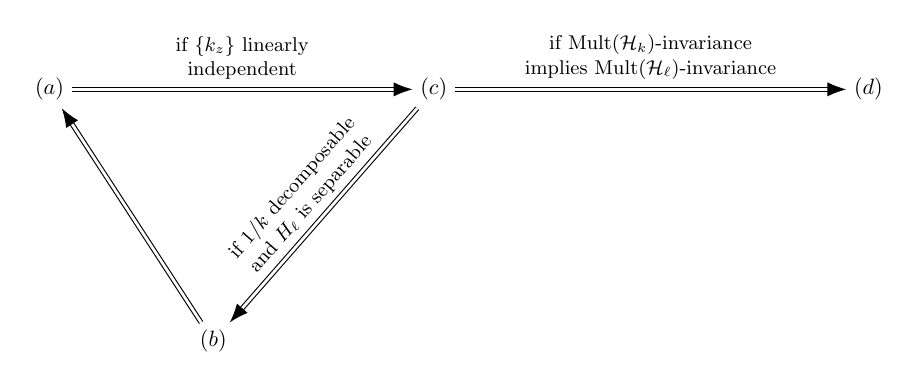
\begin{tikzpicture}[
    scale=0.80,
    every node/.style={scale=0.80},
    >=Latex,
    implication/.style={
        double distance=1.0pt,
        line width=0.4pt,
        -{Latex[length=2.4mm,width=1.8mm]}
    }
]

% Nodes
\node (a) at (0,0) {$ (a) $};
\node (c) at (6.1,0) {$ (c) $};
\node (d) at (13.0,0) {$ (d) $};
\node (b) at (2.6,-4) {$ (b) $};

% Arrows
\draw[implication]
    (a) -- node[midway, above, font=\small, align=center, text width=3.8cm, yshift=1pt]
    {if $\{k_z\}$ linearly independent}
    (c);

\draw[implication]
    (c) -- node[midway, above, font=\small, align=center, text width=7.0cm, yshift=1pt]
    {if $\Mult(\mathcal{H}_k)$-invariance $\text{implies}$ $\Mult(\mathcal{H}_{\ell})$-invariance}
    (d);

\draw[implication]
    (c) -- node[midway, sloped, above, font=\small, align=center, text width=4.4cm]
    {if $1/k$ decomposable and $H_{\ell}$ is separable}
    (b);

\draw[implication]
    (b) -- (a);

\end{tikzpicture}
\end{center}



\noindent Suppose now that $k, \ell$ satisfy Assumption \ref{assume}. The relation between the conditions above and those below, 

\begin{enumerate}[(a)] \itemsep=6pt
\setcounter{enumi}{4}
 \item    \label{i:regularAg}   $(k, \ell)$ admits an Agler decomposition; 
           \item   \label{i:co-extpair}  $(k, \ell)$ is a co-extension pair, 
\end{enumerate}

\noindent are summarized in the diagram below. 


\begin{center}
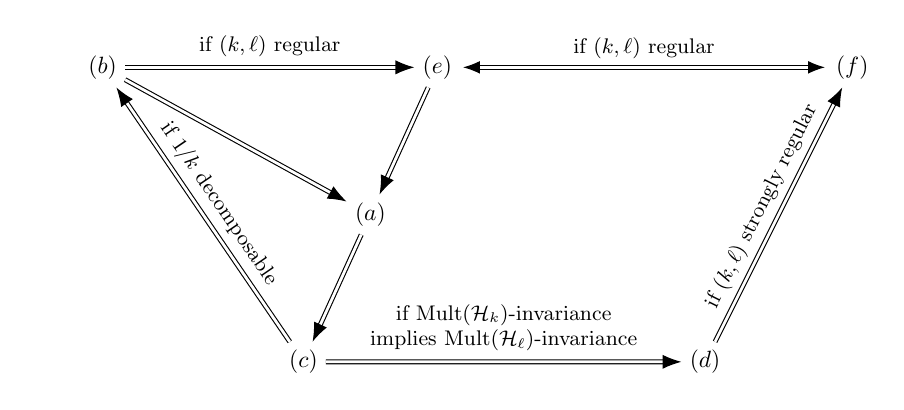
\begin{tikzpicture}[
    scale=0.85,
    every node/.style={scale=0.85},
    >=Latex,
    implication/.style={
        double distance=1.0pt,
        line width=0.4pt,
        -{Latex[length=2.4mm,width=1.8mm]}
    }
]

% Nodes
\node (b) at (0,0) {$ (b) $};
\node (e) at (5.0,0) {$ (e) $};
\node (f) at (11.2,0) {$ (f) $};

\node (a) at (4,-2.2) {$ (a) $};
\node (c) at (3.0,-4.4) {$ (c) $};
\node (d) at (9.0,-4.4) {$ (d) $};

% Main chain
\draw[implication]
    (b) -- node[midway, above, font=\small, align=center, text width=7.0cm, yshift=1pt]
    {if $(k,\ell)$  regular}
    (e);

% Arrows from (e) to (a) and (a) to (c), drawn on the right side
\draw[implication] (e) to (a);
\draw[implication] (a) to (c);

% c -> b with hypothesis
\draw[implication]
    (c) -- node[midway, sloped, above, font=\small, align=center, text width=3.3cm]
    {if $1/k$ decomposable}
    (b);
    
\draw[implication]
    (b) -- (a);
% c -> d
\draw[implication]
    (c) -- node[midway, above, font=\small, align=center, text width=7.0cm, yshift=1pt]
    {if $\Mult(\mathcal{H}_k)$-invariance $\text{implies}$ $\Mult(\mathcal{H}_{\ell})$-invariance}
    (d);

% d -> f with hypothesis
\draw[implication]
    (d) -- node[midway, sloped, above, font=\small, align=center, text width=4.2cm]
    {if $(k,\ell)$ strongly regular}
    (f);


% e <-> f equivalence, no label
\draw[double distance=1.0pt, line width=0.4pt, <->, shorten <=1pt, shorten >=1pt]
    (e.east) -- node[midway, above, font=\small]
    {if $ (k,\ell) \text{ regular} $}
    (f.west);

\end{tikzpicture}
\end{center}

\noindent In particular, if $(k, \ell)$ is strongly regular and $1/k$ is decomposable, 
then all items from (a) to (f) are equivalent. 
\end{theorem}


\begin{remark}
Recall that  $\Mult(\mathcal{H}_k)$-invariance coinciding with  $\Mult(\mathcal{H}_{\ell})$-invariance is guaranteed under very light additional assumptions (Proposition \ref{allequiv} and Corollary \ref{c:allequiv}).
\qed\end{remark}

\begin{proof}[Proof of Theorem \ref{DerSatz}]
Consider the first diagram. The implication \ref{i:Leech}$\Rightarrow$\ref{i:BLH} is Proposition \ref{LeechtoBLH};   \ref{i:weakAgler}$\Rightarrow$\ref{i:Leech} is Theorem \ref{AglerdectoLeech}; and  \ref{i:strongAgler} $\Rightarrow$ \ref{i:weakAgler} is trivial. Finally, \ref{i:Leech} $\Rightarrow$ \ref{i:strongAgler} follows from Theorem \ref{Leech=wAg=sAg}. 
Now, consider the second diagram. The equivalence \ref{i:regularAg} $\Leftrightarrow$ \ref{i:co-extpair} is Theorem \ref{COEXTISAGLER}. For \ref{i:strongAgler}$\Rightarrow$\ref{i:regularAg}, assume $1/k=Q(1-\Phi\Phi^*)Q^*$ for a function $Q$ and an operator-valued contractive multiplier $\Phi$ of $\mathcal{H}_{\ell}$. By Corollary~\ref{strongAglertoAgler}, both $Q$ and $\Phi$ can be taken holomorphic. One can then repeat, mutatis mutandis, the argument showing \ref{i:regularAg}$\Rightarrow$\ref{i:co-extpair} that is contained at the beginning of the proof of Theorem \ref{COEXTISAGLER} to obtain 
\ref{i:strongAgler}$\Rightarrow$\ref{i:co-extpair}, yielding the desired implication. The implication \ref{i:regularAg}$\Rightarrow$\ref{i:weakAgler} is trivial. The implications 
 \ref{i:weakAgler}$\Rightarrow$\ref{i:Leech}, \ref{i:Leech} $\Rightarrow$ \ref{i:BLH}
and \ref{i:Leech} $\Rightarrow$ \ref{i:strongAgler} are all proved as in the first diagram (for the proof of item~\ref{i:weakAgler} implies item~\ref{i:Leech}, notice that the needed independence of  $\{k_z\}$ follows automatically from Assumption \ref{assume}). Finally, \ref{i:BLH}$\Rightarrow$\ref{i:co-extpair} follows from Theorem \ref{BLHISCOEXT}. 
\end{proof}


\begin{remark}\rm
A direct proof of the implication \ref{i:strongAgler}$\Rightarrow$\ref{i:regularAg}
 that bypasses  regularity is possible
 with the assumption that contractive polynomial multipliers are WOT-dense in the space of contractive $\mathcal{H}_{\ell}$-multipliers. This assumption
 holds for a number of natural classes of kernels that are ubiquitous in the literature, including  regular unitary invariant kernels on the ball
  (see Example \ref{regularballex}), where one has access to Fejér's kernel. 
\qed
\end{remark}
 

\section{Examples}\label{Exampsec}
  This section contains three examples.  Example~\ref{bidiskex}
  characterizes strongly regular BLH pairs over the bidisk,
  $\mathbb{D}^2,$ whose multiplier algebra is $H^\infty(\mathbb{D}^2)$ via a criteria that flows from  Agler-Pick interpolation  on the bidisk \cite{Hellinger}.
  Example~\ref{regularballex} shows, for unitarily invariant kernels 
  $(k,\ell)$ over the ball $\mathbb{B}^\lcal{d}$ that satisfy a spectral condition and for which $M_z^\ell$ is a row contraction,  $(k,\ell)$
  is BLH if and only if the criteria of Proposition~\ref{CPinbetween} hold with $s$ equal to the
  Drury-Arveson kernel.   Example~\ref{eg:recursivel} exhibits
  a strongly regular BLH pair of diagonal holomorphic kernels that does not satisfy the 
  criteria of Proposition~\ref{CPinbetween}. See Remark~\ref{r:more} and the discussion in the preamble
  of Subsection~\ref{CPsubsec}.
  

 \begin{example} \label{bidiskex}
\pushQED{\qed}
Assume $(k, \ell)$ is a strongly regular pair on $\DD^2$ such that $\Mult(\mathcal{H}_{\ell})=H^{\infty}(\DD^2)$ isometrically. 
Recall that every holomorphic Schur function\footnote{A holomorphic Schur function is a contractive multiplier of $H^2(\DD^\lcal{d})$,
in this case with $\lcal{d}=2$.} $\Phi:\DD^2\to\mathcal{B}(\mathcal{E})$ can be represented as 
\[1-\Phi(z)\Phi(w)^*= (1-z_1\overline{w_1})G_1(z,w)+(1-z_2\overline{w_2})G_2(z,w)\]
for operator-valued kernels $G_1, G_2$ \cite{Hellinger} (see also \cite{BickelKnese}). Thus, the set of Agler decompositions of the form $(1-z_1\overline{w_1})g_1+(1-z_2\overline{w_2})g_2,$ where $g_1, g_2$ scalar-valued holomorphic kernels, is dense in 
$\mathcal{AG}(\ell)$. But it can be easily verified that the set of all such representations is closed in $\Her(\DD^2)$, and hence
\[
\mathcal{AG}(\ell)=\big\{ (1-z_1\overline{w_1})g_1(z,w)+(1-z_2\overline{w_2})g_2(z,w) \ |\  g_1, g_2\text{ holomorphic kernels}\big\}.
\]
Thus, Proposition~\ref{gensuffBLH} implies  if $(k,\ell)$ has
a weak Agler decomposition, then $(k,\ell)$ is BLH;  the implication item~\ref{i:BLH} implies \ref{i:weakAgler} gives the converse.
Hence, from the remark above, 
   $(k, \ell)$ is a BLH pair if and only if there exist holomorphic kernels $g_1, g_2$ on $\DD^2$ such that 
\[\cfrac{1}{k(z,w)}= (1-z_1\overline{w_1})g_1(z,w)+(1-z_2\overline{w_2})g_2(z,w).  \qedhere \popQED 
\]
 \end{example}



\begin{example} \label{regularballex}
Let $k, \ell$ be unitarily  invariant kernels on the ball $\mathbb{B}_{\lcal{d}}$ with 
\[ \ell(z, w)=\sum_{n=0}^{\infty}\ell_{n}\langle z, w\rangle^{n}\]
and $\lim_n\ell_{n+1}/\ell_n=1$. This assumption is fairly common in the study of
unitarily invariant spaces (see for example \cite[Section 4]{GreeneRichtSund} or \cite[Proposition 8.5]{HartzIsomorphism}).
In particular, it implies the spectral conditions $\ol{\mathbb{B}_{\lcal{d}}}= \specT(M_z^\ell).$ Let $\mathfrak{s}(z,w)=(1-\langle z, w\rangle)^{-1}$ and assume $\ell/\mathfrak{s}\succeq 0$ (equivalently, the $\lcal{d}$-shift is a row contraction over $\mathcal{H}_{\ell}\otimes\mathbb{C}^{\lcal{d}}$). \par 
Now, assume further that $(k, \ell)$ is a BLH pair. By Proposition \ref{l_m/k}, $\ell_{\mathcal{M}}/k\succeq 0$ for every $\Mult(\mathcal{H}_k)$-invariant subspace.   Using the standard multi-index
notation, $z^{\alpha} = z_1^{\alpha_1} \cdots z_{\lcal{d}}^{\alpha_{\lcal{d}}}$ and $|\alpha| 
=\sum_j \alpha_j$ for $\alpha \in \NN^{\lcal{d}},$ given
a positive integer $m,$ let
\[
  \mathcal{M}=\{f\in \cH_\ell:  \langle f, z^{\alpha}\rangle =0, \, |\alpha|\le m-1\}. 
\] 
In this case, $\ell_{\mathcal{M}}(z,w)=\sum_{n=m}^{\infty}\ell_n\langle z, w\rangle^n.$ Thus, writing $1/k=\sum_n b_n\langle z, w\rangle^n$, the condition $\ell_{\mathcal{M}}/k \succeq 0$ yields 
\begin{equation*} 
\sum_{n=0}^p b_{p-n}\ell_{m+n}\ge 0,\qquad p\ge 0.
\end{equation*}
Dividing by $\ell_m$ and letting $m\to\infty$ then obtains
\begin{equation} \label{bcoeffs}
\sum_{n=0}^p b_{p-n}\ge 0,\qquad p\ge 0,
\end{equation}
and thus $\mathfrak{s}/k\succeq 0$. By Proposition \ref{CPinbetween}, having $\ell/\mathfrak{s}\succeq 0, \mathfrak{s}/k\succeq 0$ is sufficient for $(k, \ell)$ to be BLH. We conclude that, if $(k, \ell)$ is a pair of unitarily invariant kernels on 
$\mathbb{B}_{\lcal{d}}$ such that $\lim_n\ell_{n+1}/\ell_n=1$ and the $\lcal{d}$-shift  is contractive over $\mathcal{H}_{\ell}\otimes\mathbb{C}^{\lcal{d}}$, then $(k, \ell)$ is BLH if and only if $\mathfrak{s}/k\succeq 0$ (equivalently, \eqref{bcoeffs} holds).
\qed
\end{example}



\begin{example}\rm 
\label{eg:recursivel} We now construct a strongly regular BLH pair of kernels $(k, \ell)$ on the unit disk $\DD$ such that no CP kernel $s$ exists with $\ell/s\succeq 0, s/k\succeq 0.$
First, define the reproducing kernel $k$ on $\mathbb{D}$ by
\[
 \frac{1}{k(x)} = 2(3-2x-x^2)+x^3(3-x-2x^2)
\]
 where $x=z\ol{w}.$  To see why $k$ is a   positive-definite kernel
on $\mathbb{D}$  (and hence $1/k$ is non-zero on $\mathbb{D}\times \mathbb{D}$) and at the same time $M_z$ is a bounded operator ($z$ is a multiplier),  write 
\[
k(x)=\frac{1}{(1-x)Q(x)},
\]
where $Q(x)=6+2x+3x^3+2x^4.$ Isolating the principal part ($Q(1)=13$) gives,
\[
k(x)=\frac{1}{13(1-x)}+H(x),
\]
where
\[
H(x)=\frac{7+5x+5x^2+2x^3}{13\,Q(x)}.
\]
Write
\[
k(x)=\sum_{n\ge 0} a_n x^n,
\qquad
H(x)=\sum_{n\ge 0} b_n x^n.
\]
Thus
\[
a_n=\frac{1}{13}+b_n,
\]
and it suffices to show that  $b_n> -1/13$ for all sufficiently large $n$ and  $b_n\to 0,$ and then check the remaining values of $n$ directly. Doing so immediately shows $k\succeq 0$. It also shows for sufficiently large $C>0$ that
\[
 ((C^2+1)-x)k(x) = C^2 k(x) + H(x) \succeq 0
\]
and therefore $M_z$ is a bounded operator on $\cH_k.$


Math software tells us that $Q$ has roots
\[
\rho,\ \overline{\rho},\ \sigma,\ \overline{\sigma},
\]
with
\[
\rho \approx 0.64025063148+0.97927927858\,i,
\qquad
\sigma \approx -1.39025063148+0.50865487710\,i.
\]
Their moduli are
\[
|\rho|\approx 1.17000375066\ldots,
\qquad
|\sigma|\approx 1.48038055997\ldots.
\]
The polynomial $H(x)$ has the partial fraction decomposition
\[
H(x)=\frac{A}{1-x/\rho}+\frac{\overline A}{1-x/\overline\rho}
+\frac{B}{1-x/\sigma}+\frac{\overline B}{1-x/\overline\sigma}.
\]
We obtain that the constants are approximately
\[
A=0.02358575827+0.03213408107\,i,
\qquad
|A|=0.03986084745\ldots,
\]
\[
B=0.02128603660-0.01474247235\,i,
\qquad
|B|=0.02589277593\ldots.
\]
From the partial fraction decomposition,
\[
b_n=A\rho^{-n}+\overline A\,\overline\rho^{-n}
+B\sigma^{-n}+\overline B\,\overline\sigma^{-n}.
\]
Hence
\[
|b_n|
\le 2|A|\,|\rho|^{-n}+2|B|\,|\sigma|^{-n}.
\]
Using the numerical values above,
\[
|b_n|
\le 2(0.03986084745)(1.17000375066)^{-n}
+2(0.02589277593)(1.48038055997)^{-n}.
\]
For \(n\ge 3\), the right-hand side is \(<1/13\). Therefore
\[
a_n=\frac{1}{13}+b_n>0
\qquad (n\ge 3).
\]
Checking the first three coefficients directly yields
\[
a_0=\frac16,\qquad a_1=\frac19,\qquad a_2=\frac7{54},
\]
all of which are positive. We have, in fact, shown that $(a_n)$ converges to $1/13$, 
{and thus $k$ is  a diagonal holomorphic kernel on the unit disk}.
See Appendix~\ref{append-more-example} for an analytic verification
that $a_n>0$ for all $n$ and $b_n$ converges to $0.$

 
Next, choose $\ell(x)= 1 +\sum \ell_n x^n$ as 
 follows with the aim of ensuring that both
\[
  (3-2x-x^2)\ell(x)\succeq 0, \  \ (3-x-2x^2)\ell(x) \succeq 0,
\]
 which then ensures that $1/k$ is in the Agler wedge of $\ell.$
The coefficient $\ell_1$ must satisfy both,
\[
 -2 + 3\ell_1 \ge0, \ \ -1 +3\ell_1 \ge0.
\]
Choose $\ell_1 = 2/3.$  Next, the coefficient $\ell_2$ needs to satisfy,
\[
\begin{split}
 0 & \le 3\ell_2 - 2\ell_1 -1 = 3\ell_2 - 7/3;
 \\ 0 & \le  3\ell_2 - \ell_1 - 2 =  3\ell_2 - 8/3.
\end{split}
\]
 Choose $\ell_2 = 8/9.$ It is clear that we may continue in this fashion
 to construct $\ell$:  In each iteration there are two constraints
 and the active one alternates.  For instance, 
 $\ell_3$ must satisfy both
\[
  \begin{split}
       0 & \le  3\ell_3-2\ell_2 -\ell_1 = 3\ell_3 - 16/9-2/3 = 3\ell_3- 22/9
    \\ 0 & \le  3\ell_3-\ell_2-2\ell_1 = 3\ell_3-8/9-4/3
     = 3\ell_3 - 20/9. 
  \end{split}
\]
 Hence $\ell_3\ge 22/27$ and we choose $\ell_3=22/27.$ Continuing in this way yields
 \begin{equation}
     \label{e:double-rec}
  \ell_{2k+2} = \frac{\ell_{2k+1} + 2\ell_{2k}}{3}, \ \ 
 \ell_{2k+3} = \frac{2\ell_{2k+2} + \ell_{2k+1}}{3}.
\end{equation}
 Thus $\ell$ is positive semi-definite.
 By construction $(3-2x-x^2)\ell$ and $(3-x-2x^2)\ell$ are positive semi-definite.
 Thus, $1/k$ is in the Agler wedge of $\ell$.  
 
 
 The recurrence relations of equation~\eqref{e:double-rec} leads to a closed form for $\ell.$ Indeed, setting $a_k=\ell_{2k}, b_k=\ell_{2k+1},$
  equation~\eqref{e:double-rec} becomes, 
\[
a_{k+1}=\frac{2a_k+b_k}{3},\qquad b_{k+1}=\frac{2a_{k+1}+b_k}{3},
\]
Since 
\[
4a_{k+1}+3b_{k+1}
=4\cdot\frac{2a_k+b_k}{3}+3\cdot\frac{4a_k+5b_k}{9}
=4a_k+3b_k,
\]
 $4a_k+3b_k$ is constant. At $k=0$,
$4a_0+3b_0=6$,
hence $4a_k+3b_k=6$ for all $k$.
 
Letting $d_k=b_k-a_k$ gives,
\[
d_{k+1}=b_{k+1}-a_{k+1}
=\frac{2a_{k+1}+b_k}{3}-a_{k+1}
=\frac{b_k-a_{k+1}}{3}
=\frac{2}{9}\,d_k,
\]
and thus
\[
d_k=\bigl(\ell_1-\ell_0\bigr)\left(\frac{2}{9}\right)^k
=-\frac{1}{3}\left(\frac{2}{9}\right)^k.
\]
 Solving the system
\[
b_k-a_k=d_k,\qquad 4a_k+3b_k=6
\]
gives
\begin{equation} \label{closedcoeff}
a_k=\frac{6}{7}+\frac{1}{7}\left(\frac{2}{9}\right)^k,\qquad
b_k=\frac{6}{7}-\frac{4}{21}\left(\frac{2}{9}\right)^k.    
\end{equation}
Therefore
\[
\ell(x)=\sum_{k\ge0}a_k x^{2k}+\sum_{k\ge0}b_k x^{2k+1}
=\frac{6}{7}\frac{1+x}{1-x^2}+\left(\frac{1}{7}-\frac{4}{21}x\right)\frac{1}{1-\frac{2}{9} x^2},
\]
and simplifying,
\begin{equation}\label{ellclosed}
\ell(x)=\frac{3(3-x)}{(1-x)(9-2x^2)}.
\end{equation}


To rule out the possibility of the existence of a CP kernel  $s$
and positive kernels $Q$ and $P$ such that $\ell=sQ$ and $s=Pk,$
  we argue by contradiction and assume such an $s$ exists. 
Since $\ell$ is non-vanishing, the same is true for $s$ (and $Q$
and therefore $P$). In particular, 
\[
  \ell/s = Q, \ \ \ P/s =1/k.
\]
Since $k(z,0)=1,$ it follows that $s(z,0)=1$ so that,
\[
  s(0,0)- \frac{s(z,0)s(0,w)}{s(z,w)} = 1 - B(z,w).
\]
 where $P(z,0)=0$ and $B\succeq 0$. Thus,
by Lemma~\ref{l:l/s}, without loss of generality,
\[
  1/s = I-B(z,w) = 1-\Psi(z)\Psi(w)^*,
\]
for a Hilbert space $\mathcal{K}$ and contractive multiplier $\Psi\in \Mult(\cH_\ell\otimes \mathcal{K},\cH_\ell).$ 
By virtue of being a normalized    holomorphic kernel,
the space $\cH_\ell$ contains the constant function $1$. Therefore, 
the fact that $\Psi$ is a multiplier of $\cH_\ell$ implies
$\Psi$ is analytic, and so $1/s$ is a   holomorphic kernel.
Write,
\[
1/s= 1-B(z,w) =1 - \sum_{j,k=1}^\infty b_{jk}z^j \ol{w}^k.
\]
Since $1/s, \, \ell$  and $1/k$ are holomorphic kernels, so are $P$ and $Q.$ Thus $P$ and $Q$ have power series expansions, $P=6 \sum_{j,k=0}^\infty  p_{j,k} z^j\ol{w}^k$ and $Q=\sum_{j,k=0}^\infty q_{j,k} z^j \ol{w}^k.$   From
 \[
  2(3-2x-x^2)+x^3(3-x-2x^2) = 1/k= P/s = P(1-B),
  \]
it follows that  $p_{00}=1$ and $p_{j,0}=0=p_{0,j}$ for all $j\ge 1$
and 
\[
 -4 = 6(p_{11} -b_{11}) \ge -6 b_{11}.
\]
 Thus $b_{11} \ge 2/3.$ On the other hand,
 from  $Q=\ell(1-B)\succeq 0,$ 
 \[
  0\le  q_{11} = \ell_{1}-b_{11} = 2/3-b_{11}.
\]
 Thus $b_{11}=2/3$ and $p_{11}=0=q_{11}$. Hence $p_{1j}=0=p_{j1}$
 and $q_{1j}=0=q_{j1}$ for all $j.$   Since, for $j\ge 1,$ 
\[
 0 = p_{1j}- p_{00}b_{1j},
\]
 it follows that $b_{1j}=0=b_{j1}$ for  all $j\ge 1$ too. 

 Similarly, 
\[
 -2 =  6( p_{22}-p_{10}b_{12} -p_{01}b_{21} -b_{22})
 = 6( p_{22} - b_{22}) \ge  -6 b_{22}
\]
and thus $b_{22}\ge 1/3.$ On the other hand, 
 using $-b_{22} \le -1/3,$ 
\[
\begin{split}
     0  & \le q_{33} = \ell_3 - b_{11}\ell_2 -b_{22}\ell_1 - b_{33}
    \\ & = 22/27 - 16/27 -b_{22} (2/3) -b_{33} \le 
    22/27-16/27- 2/9 = 0. 
\end{split}
\]
Hence, $b_{22}=1/3$ and $b_{33}=0.$  Since $B\succeq0$
and $b_{33}=0$ it also follows that $b_{j3}=0=b_{3j}$ for all $j.$  At this point,
\[
 \begin{pmatrix} b_{j,k} \end{pmatrix}_{j,k=0}^3
  = \begin{pmatrix} 1&0&0&0\\ 0& 2/3 & 0&0 \\ 0 &0& 1/3&0 \\0&0&0&0
  \end{pmatrix}.
\]

 
 The coefficients $\ell_4$ and $\ell_5$ are  given by
\[
 0 = 3\ell_4 - \ell_3 -2\ell_2 
  = 3\ell_4 - 22/27- 16/9 
\]
 so that
\[
 \ell_4 = 70/81;
\]
and 
\[
0 = 3 \ell_5 -2\ell_4-\ell_3 = 3\ell_5 -  140/81 - 22/27 = 206/81.
\]
Hence, 
\[
 \ell_5 = 206/243.
\]
Thus,
\[
\begin{split}
0 & \le  q_{55} =  \ell_5 - b_{11} \ell_4 - b_{22} \ell_3 -b_{33} \ell_2 -b_{44} \ell_1 -b_{55}   
\\ &  = 206/243 - 140/243 - 22/81 -b_{44} (2/3) -b_{55} 
\\ &  = (206-140-66)/243 - b_{44}(2/3)-b_{55}  = -(2/3)b_{44} -b_{55}.
 \end{split}
\]
Hence $b_{44}=0=b_{55}$ in addition to $b_{33}=0.$

We claim that $b_{nn}=0$ for $n\ge 4$ (and in particular
$B$ is diagonal) now follows 
using only $\ell/s \succeq 0$ and the already uniquely
determined values of $b_{jj}$ for $0\le j\le 5.$ Namely,
we will show  for each $m\ge 2$ that $b_{2m,2m}=0=b_{2m+1,2m+1}$
by induction, the base case $m=2$ being clear.
Assuming, for a given $m\ge 2$ that $b_{2m,2m},b_{2m+1,2m+1}=0$ holds,  
to prove the same holds with $m$ replaced by $m+1,$ recall that 
\[
 \ell_{2m+2} = \frac{\ell_{2m+1} + 2\ell_{2m}}{3}, \ \ 
 \ell_{2m+3} = \frac{2\ell_{2m+2} + \ell_{2m+1}}{3}
\]
and $\ell/s\succeq 0$ requires,
\[
 0 \le q_{2m+3,2m+3} = \ell_{2m+3} - b_{11} \ell_{2m+2} - b_{22}\ell_{2m+1} - b_{2m+2,2m+2} \ell_1 - b_{2m+3,2m+3}.
\]
 On the other hand,
\[
\ell_{2m+3} - (2/3) \ell_{2m+2} - (1/3)  \ell_{2m+1}
 = \frac{ 2\ell_{2m+2} + \ell_{2m+1} - 2 \ell_{2m+2} - \ell_{2m+1}}{3} =0.
\]
Hence $b_{2m+2,2m+2}=0=b_{2m+3,2m+3}$ and  the induction argument is complete. Hence, 
\[
 s= \frac{1}{1-(2/3)x-(1/3)x^2}.
\]
However, 
\[
s/k = 6 + 3 x^3 + x^4 - x^5/3 + O[x]^6
\]
so that $s/k$ is not positive semi-definite, a contradiction
that proves there does not exist   
a CP kernel $s$ and positive kernels $Q$ and $P$  such that $\ell=Qs$ and $s=Pk.$ 
 
 
\par 

 To use Corollary~\ref{c:AD+invariant} to verify that
  $(k,\ell)$ is a BLH pair, it only remains to observe that
  since $M_z$ is bounded on $\cH_k,$ that $k$ satisfies 
  Assumption~\ref{assume}; and, since $\ell/k\succeq0$
  (because $k/\ell$ admits a strong Agler decomposition),
   $\Mult(\cH_k)\subseteq \Mult(\cH_\ell)$ and therefore
   $\ell$ satisfies Assumption~\ref{assume} too. 
 
 
 It remains to show that $(k, \ell)$is a strongly regular pair.  First, we claim that $\ell$ satisfies the spectral condition, arguing as follows. From \eqref{closedcoeff},  $\lim_k \ell_k=6/7.$ 
It thus follows that
\[
 \lim_{n\to \infty} \frac{\ell_{n+1}}{\ell_n} =1
\]
 and therefore,
\[
 \lim_n \bigg| \frac{\ell_m}{\ell_{n+m}}
 \bigg|^{\frac{1}{n}} =1,
\]
for any $m.$ Hence, radius  of convergence of
 $\ell$ and the spectral radius of $M_z^\ell$ are both $1.$ Since $M_z^\ell$
 is a weighted shift, $\sigma(M_z^\ell) =\overline{\mathbb{D}}$ (see e.g. \cite[Proposition~15]{Shields}), which is
 also the domain of convergence of $\ell$. Note that the same holds for the shift over $\mathcal{H}_k,$ since the coefficients in the expansion of $k$ tend to $1/13.$ Finally, item ~\ref{i:annoying} of Definition ~\ref{kexhaust}  is obtained as follows. By \eqref{ellclosed},  for $0<r<1,$
\[
\frac{\ell(x)}{\ell_r(x)}
=
\frac{(1-rx)\left(1-\frac{2}{9} r^2 x^2\right)\left(1-\frac{x}{3}\right)}
{(1-x)\left(1-\frac{2}{9} x^2\right)\left(1-\frac{r x}{3}\right)}
=
F_1(x)\,F_2(x),
\]
where
\[
F_1(x):=\frac{(1-rx)\left(1-\frac{x}{3}\right)}{(1-x)\left(1-\frac{r x}{3}\right)},
\qquad
F_2(x):=\frac{1-\frac{2}{9} r^2 x^2}{1-\frac{2}{9} x^2}.
\]
Now
\[
(1-rx)\left(1-\frac{x}{3}\right)-(1-x)\left(1-\frac{r x}{3}\right)
=\frac{2}{3}(1-r)x,
\]
so
\[
F_1(x)
=
1+\frac{2}{3}(1-r)\,\frac{x}{(1-x)\left(1-\frac{r x}{3}\right)},
\]
and hence the power series of $F_1$ has nonnegative coefficients.
Also,
\[
F_2(x)
=
1+\frac{2}{9}(1-r^2)\,\frac{x^2}{1-\frac{2}{9} x^2},
\]
and thus the same holds for $F_2.$ Therefore, $\ell(x)/\ell_r(x)=F_1(x)F_2(x)$ has nonnegative   coefficients, and thus $\ell/\ell_r$
is positive semi-definite. 
\qed
 \end{example}



\section{Questions and Problems} \label{questions}

As the title suggests, we list here several questions and a problem.

\subsection{Dropping strong regularity} Assume $(k, \ell)$ is a regular pair on $\Omega,$ set $S=M^{\ell}_z$ and  consider  a $(k, \ell)$-exhaustion $(r_n, \Omega')$. If $T$ is $\text{Mult}(\mathcal{H}_{\ell})$-contractive, then so is $r_n(T)$
for each $n$ by item~\ref{i:exh:cc} of Definition~\ref{kexhaust}. Clearly, $\specT(r_n(T))\subset\Omega$. If we knew the existence of a cardinal $\omega$ such that $r_n(T)$ is the compression of 
 $\oplus_{j=1}^\omega S$ to a semi-invariant subspace, then it would no longer be  necessary to invoke Lemma~\ref{approx1-ell} (and hence, item~\ref{i:annoying} of Definition \ref{kexhaust})
in the proof of Theorem~\ref{BLHISCOEXT}. Thus, we are led to the following, of independent interest, question. 


\begin{question}
Let $\ell$ be a kernel over a domain $\Omega\subseteq\CC^{\lcal{d}}$ that satisfies Assumption \ref{assume}, with $\ol{\Omega}$ polynomially convex and $\sigma(S)=\ol{\Omega}$. Assume $T$ is $\text{Mult}(\mathcal{H}_{\ell})$-contractive with $\specT(T)\subset\Omega.$ Does  $T$ dilate to
 $\oplus_{j=1}^\kappa S$ for some cardinal $\kappa$?
\end{question}

 
\subsection{The pseudo-Pick property}

Definition \ref{Leechdef} motivates the following alternate Pick property for a pair of reproducing kernels.



 
\begin{definition}
A pair $(k, \ell)$ on a set $X$ is a \textit{complete pseudo-Pick} pair if, whenever  positive integer  $n$ and $k$, points  $z_1, \dots, z_n\in X$ and  matrices $W_1, \dots, W_n\in M_k(\CC)$ satisfy
\[(I-W_iW_j^*)k(z_i, z_j)\succeq 0, \]
there exists a contractive multiplier $\opphi{\Phi}{X}{ \mathcal{H}_{\ell}\otimes\CC^k}{\mathcal{H}_{\ell}\otimes\CC^k}$ such that $\Phi(z_i)=W_i$ for all $i$.
\qed\end{definition}
Clearly, complete pseudo-Leech implies complete pseudo-Pick. Also, $(k, \ell)$ being complete pseudo-Pick implies the same for $(k, \ell_{\mathcal{M}}),$ for any $\Mult(\mathcal{H}_{\ell})$-invariant $\mathcal{M}.$ Thus, in view of Proposition \ref{l_m/k}, to prove complete pseudo-Pick implies BLH, it suffices to show that complete pseudo-Pick implies $\ell/k\succeq 0$. This discussion motivates:

\begin{question}\label{q:pseudo-Pick}
    Let $(k, \ell)$ be a pair of reproducing kernels with $k$ non-vanishing. If $(k, \ell)$ is complete pseudo-Pick, do we have $\ell/k\succeq 0$?  
\end{question}
 \noindent 

 
In any case, 
Theorem~\ref{CPpaircharact}, Theorem~\ref{Leech=wAg=sAg} and Example \ref{eg:recursivel} together imply that  the complete pseudo-Pick property is weaker than the complete Pick property, at least for diagonal holomorphic pairs. What more can be said? Can one compare the definitions directly?

\begin{problem}
    Determine the relationship between the complete pseudo-Pick
    and complete Pick properties for pairs.
\end{problem}
 

 
\subsection{Truncating the Agler wedge}
It is the case that a kernel is a complete Pick kernel if and only if it admits solutions to every row-valued interpolation problem. In other words, the ``row-valued Pick property" automatically implies the complete Pick property (see  \cite{Pickbook} or \cite{Gregsimple}),  motivating
the following two questions.



\begin{question}
 \label{q:not-row}
Is there a regular pair $(k, \ell)$ that is BLH but such that $1/k$ is not in the Agler wedge generated by all row-valued multipliers of $\mathcal{H}_{\ell}$? 
\end{question}
\begin{question} \label{q:not-row-strong}
     If,  in the 
context of Definition~\ref{def:mult-contraction},
the inequality of equation~\eqref{vonNeumann} holds
 for all positive integers $m$ and $P\in \CC[z_1, \dots, z_{\lcal{d}}]\otimes \CC^{1\times m},$  is $T$ $\Mult(\cH_\ell)$-contractive? That is, does the inequality of equation~\eqref{vonNeumann} hold for all positive integers $m$ and $P\in \CC[z_1, \dots, z_{\lcal{d}}]\otimes \CC^{m\times m}$? 
\end{question}
\noindent The answer is yes  in the settings of
 Examples~\ref{bidiskex} and \ref{regularballex}. Note that if the answer to Question~\ref{q:not-row-strong} is yes, then Question~\ref{q:not-row} has a negative answer.
 
 
 

\printbibliography
\appendix 
\section{ Proof of WOT Montel} \label{appendMontel}



\begin{proof}[Proof of Lemma \ref{noholmontel}]
Since $\mathcal{H}_k\otimes\mathcal{E}$ and $\mathcal{H}_k\otimes\mathcal{F}$ are separable Hilbert spaces, the closed unit ball of
$\mathcal{B}(\mathcal{H}_k\otimes\mathcal{E},\mathcal{H}_k\otimes\mathcal{F})$ is WOT-compact and metrizable. Hence, the bounded sequence
$(M_{\Phi_n})$ has a WOT-convergent subsequence, which we relabel as $(M_{\Phi_n})$. Let $T\in \mathcal{B}(\mathcal{H}_k\otimes\mathcal{E},\mathcal{H}_k\otimes\mathcal{F})$ denote the limit of this subsequence. Clearly, $\|T\|\le 1.$ We will show that $T$ is a multiplication operator. Note that WOT-convergence is preserved under taking adjoints. Thus, for fixed $x \in X$ and $f \in \mathcal{F}$, 
\[
M_{\Phi_n}^*(k_x \otimes f) = k_x \otimes \Phi_n(x)^* f
\]
converges weakly to $T^*(k_x \otimes f)$. Since $k_x\otimes\mathcal{E}$ is a (WOT) closed subspace, there exists a uniquely determined vector $\Phi(x)^* f \in \mathcal{E}$ 
such that 
\begin{equation}
    \label{e:WOT-montel:1}
T^*(k_x \otimes f) = k_x \otimes \Phi(x)^* f.
\end{equation}
Since $T^*$ is contractive, equation~\eqref{e:WOT-montel:1} implies $\Phi(x)^*$ is a bounded (in fact contractive)
linear operator from $\mathcal{F}$ to $\mathcal{E}.$ 
Next, 
 for every $e \in \mathcal{E}$ and $f \in \mathcal{F}$, 
\[
\langle \Phi_n(x)e, f \rangle
= \frac{1}{\|k_x\|^2}
\langle k_x \otimes e, M_{\Phi_n}^*( k_x \otimes f )\rangle.
\]
Passing to the limit gives
\[
\langle \Phi_n(x)e, f \rangle \to \langle \Phi(x)e, f \rangle,
\]
so $\Phi_n(x) \to \Phi(x)$ WOT on $\mathcal{B}(\mathcal{E}, \mathcal{F})$, for each $x \in X$.
 Next, we show that $\Phi: X\to \mathcal{B}(\mathcal{E}, \mathcal{F})$ is a contractive multiplier. Indeed, for any $x_1, \dots, x_n\in X$ and $f_1, \dots, f_n\in\mathcal{F},$ 
  convergence of $\sum_jk_{x_j}\otimes \Phi^*_{n}(x_j)f_j$  to $\sum_jk_{x_j}\otimes \Phi^*(x_j)f_j$  in the weak topology of $\mathcal{H}_k\otimes\mathcal{E}$ gives, 
\begin{align*}
\Big|\Big|\sum_jk_{x_j}\otimes \Phi^*(x_j)f_j \Big|\Big|& \le \liminf_n \Big|\Big|\sum_jk_{x_j}\otimes \Phi^*_{n}(x_j)f_j \Big|\Big| \\ 
& = \liminf_n \Big|\Big|M_{\Phi_{n}}^*\Big(\sum_jk_{x_j}\otimes f_j\Big) \Big|\Big| \\ 
& \le \| \sum_jk_{x_j}\otimes f_j\|.     
\end{align*}
Thus $\Phi$ is a contractive multiplier. Finally, since $T^*$ and $M^*_{\Phi}$ agree on vectors of the form $k_x\otimes f,$ we conclude $T=M_{\Phi}$,  and our proof is complete. 
\end{proof}




\section{From Agler to Realizations} \label{appendLurking}


\begin{proof}[Proof of Theorem~\ref{realization.}] 
The proof is a variation on the lurking isometry argument.
It is convenient to make a slight change in notation. Let $T(w)=Q(w)^*$ and 
view $T(w)$ as an element of $\mathcal{G}$. 
By assumption, there exists a Hilbert space $\mathcal{N}$ and a function 
$R:F\to\mathcal{B}(\mathcal{N}, \mathcal{J})$ such that, for $z, w\in F,$
\[
  V(z)V(w)^*-Y(z)Y(w)^*= \, T(z)^* \big[I-\Phi(z)\Phi(w)^*\big]T(w) \, R(z)R(w)^*.
\]
Rearranging yields, for $z,w\in F,$ 
\begin{equation*} %\label{squares}
\begin{split}  
  V(z)V(w)^*+ & R(z)R(w)^*T(z)^*\Phi(z)\Phi(w)^*T(w)
\\[3pt] & = Y(z)Y(w)^*+ T(z)^* T(w)\, R(z)R(w)^*
\end{split}
\end{equation*}
Define $E(w):\mathcal{N}\to \mathcal{G}\otimes \mathcal{N}$ via
\[
 E(w) v =  T(w)\otimes v
\]
 and note that 
\[
   E(w)R(w)^* \gamma = T(w)\otimes R(w)^* \gamma 
\]
for $\gamma\in \mathcal{J}.$ Hence, for $\gamma,\delta\in \mathcal{J},$
\[
  \langle  R(z) E(z)^* E(w) R(w)^*  \gamma,\delta \rangle
  = \langle  T(w),T(z) \rangle \, \langle R(w)^* \gamma, R(z)^* \delta\rangle.
\]
 Set 
\[
 \mathcal{Z}_1=\textup{span}\Biggl\{\begin{pmatrix}
V(w)^* \\[3pt]
\big(\Phi(w)^*\otimes I_{\mathcal{N}}\big)E(w)R(w)^*
\end{pmatrix}u\ : u\in\mathcal{J},\  w\in F  \Biggl\}\subset \LK \oplus (\mathcal{F}\otimes\mathcal{N}) 
\]
 and 
\[\mathcal{Z}_2=\textup{span}\Biggl\{\begin{pmatrix}
Y(w)^* \\[3pt]
E(w)R(w)^*
\end{pmatrix}u\ : u\in\mathcal{J},\  w\in F  \Biggl\}\subset \mathcal{L}\oplus (\mathcal{G}\otimes\mathcal{N}) .
\]
Since, 
\begin{align*}
 & \Bigg\langle  \begin{pmatrix}
V(w)^* \\[3pt]
\big(\Phi(w)^*\otimes I_{\mathcal{N}}\big)E(w)R(w)^*
\end{pmatrix} u, \, \begin{pmatrix}
V(z)^* \\[3pt]
\big(\Phi(z)^*\otimes I_{\mathcal{N}}\big)E(z)R(z)^*
\end{pmatrix} v \Bigg\rangle \\[3pt]
   = & \langle V(z) V(w)^* u,v\rangle
  + \langle  R(z) E(z)^* (\Phi(z)\Phi(w)^*\otimes I) E(w) R(w)^* u,v\rangle
 \\[3pt]  =  &\langle V(z) V(w)^* u,v\rangle
  + \langle  \Phi(z)\Phi(w)^* T(w) \otimes R(w)^* u,  T(z)\otimes R(z)^*v\rangle
  \\[3pt]  =  &\langle V(z) V(w)^* u,v\rangle +  \langle \Phi(w)^* T(w), \Phi(z)^* T(z)\rangle \,
   \langle R(w)^* u,R(z)^* v\rangle 
  \\[3pt]   = &\langle \left ( V(z)V(w)^* +  T(z)^* \Phi(z)\Phi(w)^* T(w) \, R(z)R(w)^* \right) u,v\rangle
  \\[3pt]   =  &\langle \left (  Y(z)Y(w)^*+ T(z)^* T(w)\, R(z)R(w)^* \right ) u,v\rangle
  \\[3pt]   = &\Bigg\langle \begin{pmatrix}
Y(w)^* \\[3pt]
E(w)R(w)^*
\end{pmatrix}u, \begin{pmatrix}
Y(z)^* \\[3pt]
E(z)R(z)^*
\end{pmatrix}v \Bigg\rangle,
\end{align*}
we obtain  a linear isometry  $U:\mathcal{Z}_1\to\mathcal{Z}_2$ determined by
\[ 
U:  \begin{pmatrix}
V(w)^* \\[3pt]
\big(\Phi(w)^*\otimes I_{\mathcal{N}}\big)E(w)R(w)^*
\end{pmatrix}u\mapsto \begin{pmatrix}
Y(w)^* \\[3pt]
E(w)R(w)^*
\end{pmatrix}u.
\] 
Decompose $U$ as 
 \[
\begin{array}{c c}
  & \begin{array}{cc}
    \mathcal{K} & \mathcal{F}\otimes\mathcal{N}
    \end{array} \\
  \begin{array}{c}
    \mathcal{L} \\
   \mathcal{G}\otimes\mathcal{N}
  \end{array}
  &
  \left(
  \begin{array}{cc}
    A \ \ \ \ & B \  \\
    C \ \ \ \  & D \ 
  \end{array}
  \right)
\end{array}
\]
and observe that
\begin{align}
AV(w)^*+B\big(\Phi(w)^*\otimes I_{\mathcal{N}}\big)E(w)R(w)^*&=Y(w)^* \label{eq1} \\ 
CV(w)^*+D\big(\Phi(w)^*\otimes I_{\mathcal{N}}\big)E(w)R(w)^*&=E(w)R(w)^* \label{eq2},
\end{align}
for all $w\in F.$
 Since $\|\Phi(w)\|<1$ for all $w,$ the operator $I_{\mathcal{G}\otimes\mathcal{N}}-D\big(\Phi(w)^*\otimes I_{\mathcal{N}}\big)$  is invertible. Solving  \eqref{eq2} for $E(w)R(w)^*$ obtains
\begin{equation}\label{eq3}
E(w)R(w)^*=\big(I_{\mathcal{G}\otimes\mathcal{N}}-D\big(\Phi(w)^*\otimes I_{\mathcal{N}}\big)\big)^{-1}CV(w)^*.
\end{equation}
Substituting equation~\eqref{eq3} into \eqref{eq1} yields 
\begin{equation}\label{eq4}
AV(w)^*+B\big(\Phi(w)^*\otimes I_{\mathcal{N}}\big)\big(I_{\mathcal{G}\otimes\mathcal{N}}-D\big(\Phi(w)^*\otimes I_{\mathcal{N}}\big)\big)^{-1}CV(w)^*=Y(w)^*,
\end{equation}
for all $w\in F.$ Now, define $\Psi:X\to \mathcal{B}(\mathcal{K},\mathcal{L})$ by 
\[\Psi(w)^*=A+B(\Phi(w)^*\otimes I_{\mathcal{N}})\big(I_{\mathcal{G}\otimes\mathcal{N}}-D\big(\Phi(w)^*\otimes I_{\mathcal{N}}\big)\big)^{-1}C .\]
The identity of equation~\eqref{eq4} immediately yields $V(z)\Psi(z)=Y(z)$, for all $z\in F.$ \par  It remains to show that $\Psi$ is, in fact, a contractive multiplier. Define $O:X\to\mathcal{B}(\mathcal{G}\otimes\mathcal{N}, \mathcal{K})$ by $O(w)^*=\big(I_{\mathcal{G}\otimes\mathcal{N}}-D\big(\Phi(w)^*\otimes I_{\mathcal{N}}\big)\big)^{-1}C$. Equivalently,
\begin{equation}
     \label{eq:O-variant}
     C+D\big(\Phi(w)^*\otimes I_{\mathcal{N}}\big)O(w)^*=O(w)^*,
\end{equation}
for all $w\in X.$   By definition of $\Psi,$ 
\begin{equation}
    \label{e:Psi}
A+B\big(\Phi(w)^*\otimes I_{\mathcal{N}}\big)O(w)^*=\Psi(w)^* 
\end{equation}
for all $w\in X.$ The equalities of equations~\eqref{eq:O-variant} and \eqref{e:Psi} in turn, imply that $U$ maps 
\[\begin{pmatrix}
I_{\mathcal{K}} \\
\big(\Phi(w)^*\otimes I_{\mathcal{N}}\big)O(w)^*
\end{pmatrix}v  \ \  \ \ \textup{ to }  \ \ \ \ 
\begin{pmatrix}
\Psi(w)^* \\
O(w)^*
\end{pmatrix}v,
\]
for all $w\in X$ and $v\in\mathcal{K}$.
 Since $U$ is isometric,
\[ I_{\mathcal{K}}+O(z)\big(\Phi(z)\otimes I_{\mathcal{N}}\big)\big(\Phi(w)^*\otimes I_{\mathcal{N}}\big)O(w)^*=\Psi(z)\Psi(w)^*+O(z)O(w)^*, \]
which, after rearranging and multiplying by $\ell(z, w)$, becomes
\begin{align}
& \ \big[I_{\mathcal{K}}-\Psi(z)\Psi(w)^*\big]\ell(z, w) \notag \\ 
=&\ O(z)\Big(\big[I_{\mathcal{G}\otimes\mathcal{N}}- \big(\Phi(z)\otimes I_{\mathcal{N}}\big) \big(\Phi(w)^*\otimes I_{\mathcal{N}}\big)     \big]\ell(z, w)\Big)O(w)^*. \label{anothermult}  
\end{align}
 Since $\opphi{\Phi}{X}{\mathcal{H}_{\ell}\otimes\mathcal{F}}{ \mathcal{H}_{\ell}\otimes\mathcal{G}}$ is a contractive multiplier,
 \[\big[I_{\mathcal{G}\otimes\mathcal{N}}- \big(\Phi(z)\otimes I_{\mathcal{N}}\big) \big(\Phi(w)^*\otimes I_{\mathcal{N}}\big)     \big]\ell(z, w)\succeq 0,\]
 and thus \eqref{anothermult} is positive semi-definite.  Hence $\opphi{\Psi}{X}{\mathcal{H}_{\ell}\otimes\mathcal{K}}{\mathcal{H}_{\ell}\otimes\mathcal{L}}$ is a contractive multiplier, as desired. 
\end{proof}


\section{An analytic proof of positivity of \texorpdfstring{$k$}{1/k}
in example~\ref{eg:recursivel}} \label{append-more-example}
This appendix provides an analytic proof of the positivity of
$k,$ one that avoids numerical approximations of the roots
of $Q$ and the coefficients in the partial fraction decomposition
of $H.$

To prove that $Q$ has no real zeros, observe that 
\[
  M = \begin{pmatrix} 4 & 1 & -1 \\ 1 & 2 & \frac32 \\ -1 & \frac32 & 2\end{pmatrix}
    = 4 \left [ \begin{pmatrix} 1\\ \frac14 \\ -\frac14 \end{pmatrix}
    \begin{pmatrix} 1&  \frac14 & -\frac14 \end{pmatrix}+
      \frac{7}{16} \begin{pmatrix} 0&0&0\\0&  1 & 1  \\ 0& 1 & 1 \end{pmatrix} \right ]
\]
 is positive semi-definite and hence, for $x$ real, 
\[
Q(x) = {2+}\begin{pmatrix} 1 &  x &  x^2 \end{pmatrix}  M \begin{pmatrix} 1 \\ x\\ x^2 \end{pmatrix} \ge 2.
\]
 It follows that $Q$ has two pairs of complex conjugate roots, say $\rho,\ol{\rho}$ and $\sigma, \ol{\sigma}.$
 
The real part of $Q$ for $z=e^{it}$ (on the boundary of the disk) is
\[
  h(t) = 6 + 2\cos(t)+3\cos(3t)+2\cos(4t) = 
   8-7x-16x^2+12x^3+16x^4= g(x),
\]
 where $x=\cos(t).$  Let 
\[
  M(y) =\begin{pmatrix} 11/2 & - 7/2 & -8-y \\
    -7/2 & 2y & 6\\ -8-y & 6 & 16\end{pmatrix}
\]
 The upper $2\times 2$ block is psd for $y>\frac{49}{44}$
 and  
 \[
 \det(M(y)) =1/4 (-8 y^3 - 128 y^2 + 360 y - 232)
 \]
  so that 
\[
 \det(M(5/4)) >1/2. 
\]
 Hence the polynomial,
 \[
  \frac{11}{2}-7x-16x^2+12x^3+16x^4 \ge 0
 \]
  for all $x$ and therefore $g(x)\ge 5/2$ for all $x$


 Now, the strong form of Rouché's Theorem {(the $|f(z)+g(z)|<|f(z)|+|g(z)|$ version)} applies to $f=Q$ and $g=-1$ 
 and the closed unit disk (since $f$ is never a positive multiple of $g$ 
 on the boundary) with the conclusion that  $Q$ has no zeros in the closed unit disk.


Next, for $0<s \le 1/8,$ 
 the real part of $Q((1+s) e^{it})$ is
 \[
 \begin{split}
  6+ & 2(1+s)\cos(t)+3(1+s)^3 \cos(3t)+ 2(1+s)^4\cos(4t) 
  \\ &  = h(t) +  2s\cos(t) + (3s+3s^2+s^3)\cos(3t) + (4s+6s^2+4s^3+s^4)\cos(4t)
\\  & = h(t)+F(s,t), 
\end{split}
\]
where
\[
\begin{split}
 F(s,t)= 2s\cos(t) & + (8s+9s^2+3s^3)\left(\cos(3t)+\cos(4t)\right)
  + s\cos(3t) \\ & + (3s^2+5s^3+2s^4)\cos(4t).
 \end{split}
\]
 Making the substitution $x=\cos(t),$
\[
 \cos(3t)+\cos(4t)  = 8x^4+4x^3 -8x^2-3x+1 = f(x).
\]
  The matrix
 \[
   M=\begin{pmatrix} 2.82 & -1.5 & -4.5\\
      -1.5 & 1 & 2 \\ -4.5 & 2 & 8 \end{pmatrix}
 \]
 is psd since its determinant is $.03$ and 
 the determinants of the principal minors are also positive definite. It follows that
\begin{align*}
f(x) + 1.82 &= 8x^4+4x^3 -8x^2-3x+2.82  \\
&=\begin{pmatrix}
1 & x & x^2
\end{pmatrix} M \begin{pmatrix}
1 \\ x \\ x^2
\end{pmatrix}  \\
&\ge 0
\end{align*}
 for all $x$ and hence
\[
 \cos(3t)+\cos(4t) + 1.82 \ge 0
\]
 for all $t.$
  For $t\in [-\pi/2,\pi/2],$ where $\cos(t)\ge 0,$  and $0<s \le 1/8,$
\[
  h(t) +  F(s,t) \ge 
  5/2 -(1.82)(8s+9s^2+3s^3) - (s+3s^2+5s^3+2s^4) >0,
\]
where we have used $h(t)\ge 5/2.$
  With $r(x)=f(-x)= 8x^4-4x^3-8x^2+3x+1$ and
  $\psi=r+1,$ routine calculus shows, for $0\le c \le 1,$
  that
\[
 \psi^\prime(c) \ge -25
\]
  and therefore, for $0\le x \le 1,$
\[
  \psi(x+h) \ge \psi(x)-25h.
\]
  Choosing $h=.01$ and verifying that $\psi(nh)-0.25 \ge 0$
  for $n=0,\dots,99$ shows $\psi \ge 0$ on the interval
  $[0,1].$ Hence  $f(x) >-1$ on the interval $[-1,0]$
  and consequently, for $t\in [\pi/2,3\pi/2]$ and $0<s \le 1/8,$
\[
  h(t) + F(s,t) 
  \ge 5/2 - (8s+9s^2+3s^3) - (3s+3s^2+5s^3+2s^4) >0.
\]
We conclude that the smallest modulus of a root of \(Q\) is at least
\(\frac{9}{8}\). Since every root of \(Q\) has modulus at least
\(\frac{9}{8}\), and since the product of the four roots is \(3\)
(the constant term of the monic polynomial associated with \(Q\)),
it follows that every root has modulus at most
\begin{equation}
    \label{e:max-mod-Q}
\sqrt{3}\,\frac{8}{9}  < 1.54.
\end{equation}




 Let  $z=a+ib$ denote  a root of $Q$ and  let $R(x,y)$ and $I(x,y)$
 denote  the real and imaginary parts of $Q$ respectively
 (where $z=x+iy$), then, from 
\[
\begin{aligned}
Q(z) &= 6 + 2(a+bi)
      + 3\!\left[(a^{3}-3ab^{2}) + (3a^{2}b-b^{3})\,i\right] \\
     &\quad+ 2\!\left[(a^{4}-6a^{2}b^{2}+b^{4}) + (4a^{3}b-4ab^{3})\,i \right],
\end{aligned}
\]
collecting the real and imaginary parts separately gives,
\[
\begin{aligned}
R(a,b) &=
  (6 + 2a + 3a^{3}  + 2a^{4}) + ( - 12a^{2}b^{2} - 9ab^{2} + 2b^{4})
   = Q(a) + T(a,b), \\[6pt]
I(a,b) &=
  2b + 9a^{2}b - 3b^{3} + 8a^{3}b - 8ab^{3}
\end{aligned}
\]
 and we make the following observation based on $R.$ Since
 $-12a^2 -9a = -12a(a+ \frac{3}{4})>0$ for $-3/4 < a < 0,$ 
 it follows that  $T(a,b)> 0$ for $0<a<-3/4$ and $b\neq 0.$ Hence $R(a,b)> 0,$
 for $-3/4<a<0.$  On the other hand, since the sum of the real parts of the roots of $Q$ is $-\frac32,$ 
  one of the conjugate pairs of roots has negative real parts and the other conjugate pair has
  positive real parts. Let $r_j \pm i s_j$ denote the four roots
  with $r_1 \le -3/4$ and $r_2>0.$ 

 We now determine lower bound(s) for $|b|.$ Rearranging, $I(a,b)$ gives,
\[
 b^3(3+8a)=b(2+9a^2+8a^3).
\]
 Since $Q>0$ on the real axis, $b\ne 0.$ 
 In particular, $3+8a\ne 0,$ since the right hand side is not
 zero for $a=-3/8.$ 
Solving for $b^2,$ 
\[
 b^2 =\frac{2+9a^2+8a^3}{3+8a} = r(a)
\]
In the case that $-3/8 <a,$ we have $-3/8 \le a\le 1.59,$
since the real part of a  root is at most its magnitude.

In this interval, the minimum of $r(a)$ is achieved in
$[0,1.59].$ Since, for $a\ge 0,$
\[
  2+9a^2+8a^3 -(1/2)(3+8a) = \frac12 -4a + 9a^2 +8a^3
  = (\frac{1}{\sqrt{2}} - 2\sqrt{2} a)^2 + a^2 +8 a^3 >0,
\]
 we conclude that $r(a)-\frac12 \ge 0$ and hence $|b|\ge 1/2.$


 If $a\le -3/8,$ then $-1.59 \le a \le -\frac38.$ For $a$ 
 in this interval and $b$ fixed,
\[
 T(a,b)= -9ab^2-12 a^2 b^2 + 2b^4 =(-9a-12a^2)b^2+2b^4
\]
 is minimized at $a=-1.59$ with value
 \[
   T_{\text{min}} = -16.0272 b^2+2b^4.
 \]
 It follows that $T(a,b)>-2$ for $|b|\le .35.$
Summarizing. Either $a>0$ or $a<-3/4.$  Further, if $a>0,$ then $|b|>1/2$ and if $a<-3/4,$ then $|b|>.35.$ 


We now seek lower bounds on $|a|.$  For $0 \le a\le \frac{9}{17},$ 
\[
 I(a,1) = 2+9a^2+8a^3 -3-8a=-1 -8a + 9a^2+8a^3 \le -1-8a+17a^2 = r(a)
\]
 and the roots of $r(a)$ are $\frac{1}{17} ( 4\pm \sqrt{33}).$
 Since
 \[
 \frac{1}{17}(4+\sqrt{33}) > \frac{9}{17} > \frac{1}{17}(4-\sqrt{33}),
 \]
  it follows  that
\[
 I(a,1)\le  r(a)<0 
\]
  for $0\le a\le \frac{9}{17}.$ 
On the other hand, for $0\le a\le \frac{9}{17}$ and $b\ge 1,$
\[
\begin{split}
 \frac{\partial I}{\partial b}(a,b)  & =(2+9a^2+8a^3) - (9+24a)b^2
 \\ &  < -7 -24a + 9a^2 + 8 a^3 < -7 + 9 (9/17)^2 + 8(9/17)^3  < 0. 
\end{split}
\]
 We conclude that $I(a,b)< 0$ for $0\le a\le \frac{9}{17}$ and $b\ge 1.$ 
 Consequently, if $z=a+bi$ is a root and $a,b>0,$ then  $b<1.$ From
 $a^2+b^2 \ge (12/11)^2,$ we conclude that $a\ge \sqrt{23}/{11}.$
 Hence, the real part of the roots of $Q$ with positive real part is at least $\sqrt{23}/{11}$.

  Summarizing, for the  roots $r_1\pm i s_1$  we have $r_1 \le -3/4$
  and $|s_1| \ge 1/3;$ 
  and for $r_2\pm i s_2,$ we have 
  $r_2\ge  \sqrt{23}/{11}$ and $|s_2|\ge 1/2.$ 

 Now, for any three roots $w_1,w_2,w_3$ of $Q,$  
\[
|w_1-w_2|\, |w_2-w_3|\, |w_3-w_1| \ge  
  \Big(\frac{2}{3}\Big)\Big(\frac34+\cfrac{\sqrt{23}}{11}\Big) 
   \left (\Big(\frac{5}{6}\Big)^2 + \Big(\frac34+\frac{\sqrt{23}}{11}\Big)^2\right)^\frac12
   \ge 1.4
\]
  Moreover, letting $w_4$ denote the remaining root, 
  from the inequality of equation~\eqref{e:max-mod-Q},
\[
 3= |w_1w_2w_3|\, |w_4|  \le |w_1 w_2 w_3| \sqrt{3}\frac{8}{9},
\]
from which it follows that 
\[
|w_1w_2w_3|\ge \sqrt{3}(9/8).
\]
Thus the  coefficient $A$ corresponding to the root $w_4$
 in the partial fraction decomposition of $H$ satisfies
\[
 |A| = \bigg|\frac{N(r_4)}{13 w_1 w_2 w_3 (w_1-w_2)(w_2-w_3)(w_3-w_1)}\bigg| 
 \le \frac{8\cdot N(1.54)}{13\cdot 9 \cdot(1.4) \sqrt{3}}
 \le 1.005.
\]

 
 
  Since the same inequality holds for each of the other
 three terms in the partial fraction decomposition of $H,$
 letting $\rho$ and $\sigma$ denote the magnitudes
 of the roots of $Q$ with positive and negative real
 parts respectively and using $\rho \sigma=\sqrt{3},$ 
 \[
 |b_n| \le 2 \cdot (1.005)[ \rho^{-n} + (\frac{\rho}{\sqrt{3}})^n. ]
 \]
  Maximizing over $\frac{9}{8} \le \rho \le \sqrt{3}\frac{11}{12}$
  and using the maximum occurs at the endpoints and 
  the estimate for $|b_n|$ decreases with $n,$
\[
 |b_n| \le  (2.01) [ (8/9)^n + (9/(8 \sqrt{3})^n) ]
 <1/13
\]
  for $n\ge 28.$  Now one checks that $-1/13 < b_n$
  for 
  $n\le 27.$  See the power series expansion for $H(x)$ below.

\bigskip

\begin{equation*}
\begin{split}
0.0897436 & + 0.034188 x + 0.0527066 x^2 - 0.0367996 x^3 - 0.034742 x^4 - 0.0261686 x^5  
\\  &+ 0.00955383 x^6 + 0.0264529 x^7 + 0.0158473 x^8 - 0.00133649 x^9
\\ & - 0.0159656 x^{10}
 - 0.0114195 x^{11} - 0.000807717 x^{12} + 0.00869753 x^{13}
 \\ &+ 0.00813241 x^{14} + 0.00149954 x^{15}
 - 0.00457937 x^{16} - 0.00543892 x^{17}
 \\ & - 0.0016476 x^{18} + 0.00233904 x^{19} + 0.00346624 x^{20} + 0.00148136 x^{21}
 \\ & - 0.00111411 x^{22} - 0.00214143 x^{23} - 0.00118228 x^{24}
 + 0.000457361 x^{25}
 \\  & + 0.00128963 x^{26} + 0.000875075 x^{27} +O(x^{28}).
 \end{split}
 \end{equation*}

 \newpage

 \printindex
 \end{document}
 



 
